\clearpage
\part*{Part IX. The Junction\\[5pt]{\large The (3,3) cell}}
\label{atlaspart:09-cell-3-3-strong}
\addcontentsline{toc}{part}{Part IX. The Junction, The (3,3) cell}
\section*{Introduction to Part IX}\label{narr:part:VII}
\addcontentsline{toc}{section}{Introduction to Part IX}
The strong interaction sits at the cell (3,3) of the register matrix, the genre that pairs two qutrit ends and is the one genre at which no read survives at the first order. Part IX reads that fact as confinement, and then builds outward from it: the strong coupling as a closed read through the hadron body, the structure of the nucleon as a census of star records, the proton as a seeded sink, the ratio of the proton to the electron as a candidate read at second order, the hadron spectrum as a roster of saturated joined webs, the quark content and its flavors, and two chapters reserved for chiral breaking and the cap. The Part is the place where the saturation of chapter 1-5 does its heaviest work, because every hadron here is a sink of a seeded web.

The order of the nine chapters is dictated by one object, the star. A hadron in this construction is a star, a junction qutrit of degree three carrying the three quark bodies of the roster at its leaves, with the docks of the bodies its pendant pairs, and the quark is a body at the dark legs of that star. Confinement is read first because it is a statement about the legs of the star, the coupling second because it is a closed read through the star, the nucleon third because the star is counted record by record, the proton fourth because the star is seeded and saturated, and the mass ratio fifth because it is read at the second order at the same star. The spectrum and the quark content widen the view from one star to the joined webs of several stars and to the bodies at the leaves. The two chapters at the end are reserved, and the introduction names them as such. A reader who wants to see how far a finite construction can carry the strong interaction without a field should read chapters 7-1 and 7-4 together, the first for why no read survives at first order and the second for what the saturation does with that fact.

Chapter 7-1 reads confinement as the dark-genre readability in Theorem~171.1, resting on the link, the readability order and the probe, with the four readings beside, Open result~171.2, as an open result. The quark is a body at the dark legs of the star, the qutrit-qutrit links of the dark genre, and the readability of that genre is what confinement names, Theorem~171.1. The open result beside it types the dark-link cut by the read order of the cut link, first order at the qutrit-qubit genre at 162 of the 6296 cuts and second order at the dark genres at 6134, so that the construction admits a dark-link cut at the first order not, and at every dark cut the engine at order two reads the cut link with the twenty-eight records of the genre, Open result~171.2. Chapter 7-2 reads the strong coupling as the gluon closed read through the hadron body, Theorem~172.1, and states the running and the one genre per force, Open result~172.2, as an open result. The gluon closed qutrit-qutrit read at its pair is the closure sector twenty-eight at the gain three inside the chain sum, the coupling of the qutrit-qutrit genre an exact element of the field over the slot star with its order-two readout over the star, Theorem~172.1. The open result finds that the saturated proton carries no first-order colored readout at its three core legs, that the running reaches the Z body at no rung of the register tower, the Z body standing off the tower between the fourth and fifth rungs, and that one genre per force holds at the electromagnetic alone, Open result~172.2. These two chapters fix the (3,3) cell of the register matrix: the identification algebra su(3)+su(3)+u(1), the first non-vanishing read at order two, and the strong coupling as the office of the gluon pair ket, by name.

Chapters 7-3 to 7-5 read the nucleon. Theorem~174.1 reads nucleon structure as the star record census, Theorem~174.2 the junction sharing, the register, the form factor, the office and the pairable legs, with the five readings beside, Open result~174.3. The proton star, read link by link at the slot polarity, carries three thousand eight hundred fifty-seven records, each typed at an order, Theorem~174.1. At every one of the 250 junction sites of the roster the flat reduced diagonal of the pair ket at dimension three gives each leg one third of an end, the three thirds summing to one, and the register of the nucleon follows from the junction star at the share reading, the proton at 85 and the neutron at 125, Theorem~174.2. Open result~175.1 states the seeded saturation of the proton web as an open result, Theorem~175.2 the joined read at the roster stars, and Open result~175.4 the cap census at the proton sinks. The proton seed, the hub-attached three-quark web at the star core with the pair hub, ten sites and twelve links, is its own sink at wave zero at the stop condition of the pairing move, while under the twenty-eight catalogued moves the closure grows to twenty-five thousand five hundred fifty-eight webs, Open result~175.1. The roster stars of the proton and the neutron, each joined at the dock to the measurement web of its row, give the direct record sum to order three at the dock unit, every order exact and signed and the order-three term zero at every reading, Theorem~175.2. At every link of every proton sink of the roster census, seven webs at 80 links with 19 open docks, the record count at the primary map reading equals the cap of its genre at all 80 links, the colored links capped at all 22, Open result~175.4. Theorem~176.1 reads the mass ratio at the second-order read, a candidate and not a theorem, with its six readings beside in Open result~176.2. The lepton bodies are met again, the order of the read is exact and the ratio at the second-order read is exact, and the compendium displays the comparison nowhere, Theorem~176.1. Among the readings beside, the two ticks are exact and their squared ratio is two at the adopted unit, but the one unit tying the lattice step of the order register to the Killing norm of a direction step is fixed by no result of this work, the same missing unit the boost open result of Part IV names, Open result~176.2.

Chapters 7-6 and 7-7 widen the view to the spectrum and the quarks. Theorem~177.1 reads the hadron spectrum as the roster of saturated joined webs, Theorem~177.2 the mixed composition, the meson apparatus and the corollaries, and Open result~177.3 the direct sum at the deuteron as an open result. At the pairable set of the nucleon star, two docks at the proton star and one at the neutron star, the pairing move builds, up to four stars, exactly the joined webs admitted, and its sinks are exactly the saturated webs found, among them the chains of two neutron stars, of a proton between two neutrons and of two protons between two neutrons, Theorem~177.1. The register of the common support, sixteen at every qutrit-qubit dock and eighty-one at every qutrit-qutrit leg, is derived at the fourteen docks and the twelve legs of the six docked quark bodies and the two nucleon stars as one register at each reading, Theorem~177.2, while the direct two-exchange sum at the deuteron web meets the deuteron office of the earlier result at neither binding entry, the meson web direct sum being defined at every one of the twenty-one pairings of two qutrit cores admitted at the valence bound, Open result~177.3. Theorem~181.1 reads the quark register at the second-order junction read and Theorem~181.2 flavor as the rung name with the quark ladder, with the ladder at the saturated sinks in Theorem~181.4 and the quark offices as the star arm reads in Theorem~181.5, a theorem. The read engine run through every junction star at order two reads every leg with the entering link at the cut register, so the junction entry of a second read link is one exact object, eight at the cut reading, equal to the cut-reading bound at every one of the six quark bodies, with the share the color third, Theorem~181.1. Flavor is the rung name read at the corner, the three corner frames of the charged-lepton dark triangle at one, two and three hub legs equal to the three residues of the adopted naming at every corner, Theorem~181.2. The four heavy-flavor first powers, the strange, the charm, the bottom and the top, are outputs of the hub lowering at the saturated sinks, each a rank multiplied by a dressing, Theorem~181.4, and at the primary reading every arm of the two catalogued stars and every heavy sink is an office by the body-alone rule, the six arms at the first power 319 with the up and the down equal at the ratio one and every ratio among them an exact rational cell, Theorem~181.5. Chapters 7-8 and 7-9 are reserved, the table titled The chiral-breaking chapter (in chapter~\ref{mod:VII-8-chiral-breaking-and-the-theta-angle}, among the instruments) and the table titled The cap chapter (in chapter~\ref{mod:VII-9-mesons-and-the-nucleon-at-the-cap}, among the instruments): chiral breaking, the theta angle and the cap are named there, and the cap chapter carries six results at their own standing.

In the language of the literature, this Part names confinement, the strong coupling, the gluon, the nucleon form factor, the proton-to-electron mass ratio, the hadron spectrum, the mesons, the quarks, flavor, chiral breaking and the theta angle. The correspondence is by name at each. The boxes establish censuses of records at seeded sinks and reads at second order, and the candidate of chapter 7-5 is stated as a candidate.

The dependency lines of the Part point back to the link, the records, the probe and the saturation of Part I, and forward to the body-alone office rule of chapter 8-2, which the quark offices rest on. Confinement rests on the link, the readability order and the probe. The coupling rests on confinement, the quark register and the nucleon. The proton chapter rests on the saturation and the moves, and the spectrum on the proton and the pairing move. The reader who follows the derivation graph will find the proton of chapter 7-4 near the end of one of the longest chains in the compendium, and will find that the one number the Part is most often asked for, the mass ratio, is the one result the Part is most careful to call a candidate.
\section{Confinement as the dark-genre readability}\label{mod:VII-1-confinement-as-the-dark-genre-readability}
\chdesig{9-1}{7-1}{VII-1-confinement-as-the-dark-genre-readability}{VII-1-confinement-as-the-dark-genre-readability}
\label{narr:open:7-1}Confinement is read as a readability. Theorem~171.1 reads it as the dark-genre readability of the cell (3,3), the genre at which no read survives at the first order, and Open result~171.2 states the four readings beside as an open result.
\begin{chconditional}[Confinement as the dark-genre readability]\label{box:VII-1-confinement-as-the-dark-genre-readability:1}
Under the one-act clause and the open results it rests on, the hadron of the compendium is a star, a junction qutrit of degree three carrying the three quark bodies of the roster at its leaves, with the docks of the bodies its pendant pairs; the quark is a body at the dark legs of that star, the qutrit-qutrit links of the dark genre. At every one of the 494 qutrit-qutrit links of the roster the read engine carries no first-order readout and carries the second-order read, with the readout equal to the catalogued cells at every one of the 1368 dark cuts; at every one of the six quark bodies the open qutrit-qutrit end carries no first-order rest energy; and at every one of the eight stars a first-order Born reading passes through the qutrit-qubit docks alone. Confinement is therefore a corollary of the readability typing: the hadron masses are first-order objects, the proton register 85 and the neutron 125, and the quark offices are second-order objects, a quark appearing at the first order at no reading of the construction.
\end{chconditional}
\chstanding{conditional theorem}
\chdeps{Definitions 1.1 to 1.6, Theorems 9.1 to 9.7 and Open result 9.8 and Theorems 28.1 and 28.2, Open results 28.3 and 28.4 and Theorem 28.5}{Theorem 27.1, Theorem 172.1 and Open result 172.2, Theorems 174.1 and 174.2 and Open result 174.3, Open result 175.1, Theorem 175.2 and Open result 175.3, Theorems 181.1 and 181.2 and Open result 181.3 and Open result 257.1}
The box turns confinement into a statement about which links can be read at first order, the links of the genre a quark hangs from cannot, the links a hadron's docks are made of can, so a hadron shows up at first order and a quark never does.
\begin{chwall}[The four readings beside]\label{box:VII-1-confinement-as-the-dark-genre-readability:2}
The dark-link cut is typed by the read order of the cut link, first order at the qutrit-qubit genre at 162 of the 6296 cuts and second order at the dark genres at 6134, so the construction admits a dark-link cut at the first order not; at every dark cut the engine at order two reads the cut link with the twenty-eight records of the genre, and yet the change of the structure counts across a cut is not the change of the second-order reads at the deciding comparison; the star key at the dark cut is open at its deciding step; and the confined state with both ends open stands as an open result.
\end{chwall}
\chstanding{open results, four, built and not closed}
\chdeps{Definitions 1.1 to 1.6, Theorems 9.1 to 9.7 and Open result 9.8 and Theorems 28.1 and 28.2, Open results 28.3 and 28.4 and Theorem 28.5}{Theorem 27.1, Theorem 172.1 and Open result 172.2, Theorems 174.1 and 174.2 and Open result 174.3, Open result 175.1, Theorem 175.2 and Open result 175.3, Theorems 181.1 and 181.2 and Open result 181.3 and Open result 257.1}
The second box names the four readings beside the theorem that are tried and parted at their named steps.
\begin{chbridge}
What this chapter calls the readability typing of the dark genre the literature calls color confinement, the star a hadron, the body at a dark leg a quark and the qutrit-qubit docks the valence structure. The correspondence is by name.
\end{chbridge}
\begin{chproof}[census]
The premises are the link and its six genres of chapter 1-2 and the read at a register of chapter 1-6, definitions, the chain from the axiom five chapters long. The set counted is the set of links of the catalog, 1691 across the six genres,
\begin{equation}
1691 = 255 + 54 + 657 + 494 + 219 + 12
\end{equation}
at the genres (2,2), (2,3), (2,4), (3,3), (3,4) and (4,4), with the registers whole 16, 36, 64, 81, 144, 256 and cut 9, 24, 45, 64, 120, 225. The property tested is whether the read engine carries a first-order readout at the link, present if and only if the genre is in the readable set, the genres (2,2) and (2,3), and absent at the four dark genres. By kind. At the 494 links of the genre (3,3) the first-order readout is absent at 494 of 494 and the second-order read present at 494 of 494, the catalog of records at that genre 412 with the closed form of the count law
\begin{equation}
\frac{268 + 200\sqrt{3}}{419904}
\end{equation}
equal at 494 of 494. The reads of the construction at first order are 309, 255 at (2,2) and 54 at (2,3), at 0 links of the genre (3,3). At the six quark bodies, in the order up, charm, top, down, strange, bottom, the open (3,3) end stands at 6 of 6 with no first-order rest energy at 6 of 6, and at the eight stars a first-order Born face passes through the (2,3) docks at 8 of 8. The smallest cases are the proton and the neutron stars, the proton register 85 at the share face equal to the link sum, the neutron 125, the reduced factor and the Born factor
\begin{equation}
\frac{85}{85 + 67} = \frac{85}{152}, \qquad \frac{85^{2}}{85^{2} + 67^{2}} = \frac{7225}{11714},
\end{equation}
with 67 the electron unit, and the quark office a second-order object at the junction read, the read at the (3,3) end $67/82944 + 25\sqrt{3}/41472$ and its share over three legs $67/248832 + 25\sqrt{3}/124416$, equal to the recorded share at the nucleon legs at 6 of 6.

The four counts together, the first-order readout absent at every (3,3) link, the second-order read present at every one, no first-order rest energy at the open end of any quark body and a first-order Born face at every star, make confinement a corollary of the typing, the first link with a first-order readout, the first quark body with a first-order rest energy and the first body without an open (3,3) end all none.

\emph{Check.} The first cut of this entry stood beyond its own pin and was set aside, its content confirmed at a disjoint route at 0 differing cells over 2212, and the re-fire inside the pin reproduced every cell. The result was reproduced by an independent route, two engines at every capture byte for byte, its five counter-tests and twelve controls at their pinned letters.
\chcert{494}
\end{chproof}
\label{chend:VII-1-confinement-as-the-dark-genre-readability}
\par\medskip\noindent{\itshape Confinement read, the next chapter reads the coupling of the sector.}\label{narr:close:7-1}\par
\section{The strong coupling}\label{mod:VII-2-strong-coupling}
\chdesig{9-2}{7-2}{VII-2-strong-coupling}{VII-2-D543568-scds-t1}
\label{narr:open:7-2}Theorem~172.1 reads the strong coupling as the gluon closed read through the hadron body, and Open result~172.2 states the running and the one genre per force as an open result.
\begin{chconditional}[The strong coupling as the gluon closed read through the hadron body]\label{box:VII-2-strong-coupling:1}
Under the carrier as the closed-genre read, the coupling genre, confinement, the quark register and the nucleon mass, the gluon closed qutrit-qutrit read at its pair is the closure sector twenty-eight at the gain three inside the chain sum, the coupling of the qutrit-qutrit genre an exact element of the field over the slot star and its order-two readout over the star; the read rule of that genre follows from the readability typing, the legs of a qutrit-qutrit junction read at first order at none of three and at second order at three of three at both nucleon stars, and the strong coupling as the gluon closed read through the hadron body is defined at one reading of the derived read rule, with the register of the common support, sixteen at every qutrit-qubit dock and eighty-one at every qutrit-qutrit leg, derived from the link dimensions of the roster.
\end{chconditional}
\chstanding{conditional theorem}
\chdeps{Definitions 1.1 to 1.6, Theorems 9.1 to 9.7 and Open result 9.8 and Theorem 171.1 and Open result 171.2}{Theorem 173.1 and Theorems 177.1 and 177.2 and Open result 177.3}
The box defines the strong coupling of this compendium, the gluon is the closed read of the qutrit-qutrit genre, its closure sector is one exact number of the ring, and passing that read through the proton or the neutron at the register the common support fixes gives one exact element of the field at each face. The first reading of the same object at the first row of this entry is carried whole.
\begin{chwall}[The running and the one genre per force]\label{box:VII-2-strong-coupling:2}
The saturated proton carries no first-order coloured readout at its three core legs, and the running reaches the Z body at no rung of the register tower, the Z body standing off the tower between the fourth and fifth rungs; and one genre per force holds at the electromagnetic alone, the strong coupling being the root of no single genre at any register, its body factor passing five genres at the hadron body.
\end{chwall}
\chstanding{open results, two, built and not closed}
\chdeps{Definitions 1.1 to 1.6, Theorems 9.1 to 9.7 and Open result 9.8 and Theorem 171.1 and Open result 171.2}{Theorem 173.1 and Theorems 177.1 and 177.2 and Open result 177.3}
The second box names the two readings beside that part, the running of the coupling never lands on the Z body, and the strong force is not carried by one genre the way the electromagnetic one is.
\begin{chbridge}
What this chapter calls the gluon closed read the literature calls the strong coupling, the closure sector its value at the hadron scale and the register tower the renormalization scale, each the nearest object. The correspondence is by name, and the value of the coupling stands in the comparison table alone.
\end{chbridge}
\begin{chproof}[finite computation]
The premises are the link and its six genres of chapter 1-2, a definition, confinement of chapter 7-1, a theorem, and the framework. The chain from the axiom to this chapter is six chapters long. The procedure. The input is the count law of the (3,3) genre from its two end dimensions alone, the traceless slots 8 and 8, the roster 384 and the swap-fixed 16, the sectors odd 184, mixed-even 128, same-even 72 and closure 28 at the orders 0, 1, 1 and 2 and the gains 1, 3, 3 and 9,
\begin{equation}
412 = 184 + 200 + 28, \qquad 1036 = 184 \cdot 1 + 200 \cdot 3 + 28 \cdot 9 ,
\end{equation}
the records and the Born face, with the whole 81, the cut 64 and the star of order one $419904 = 81 \cdot 72^{2}$ and of order two $331776 = 576^{2}$. The enumeration takes the gluon word at its one qutrit-qutrit link, the carrier at the closed read with the closure sector 28 at the gain 9, and the two nucleon stars, the center at dimension 3 with three (3,3) legs at the register 9 each and the arms the cataloged quark bodies at their leaves, the proton at 11 sites, 11 links and the measure 85 with the arms up, up and down at the arm sum 150, the neutron at 15 sites, 16 links and the measure 125. The test reads the legs at both orders, the first-order leg count 0 of 3 and the second-order count 3 of 3 at both stars. The aggregation composes the closed read through the body at the register of the common support, the dock register 16 at the ratio one and the port register 81 at the ratio 81 over 16. The smallest instance is the share at one leg, one third of the junction read,
\begin{equation}
\frac{67}{248832} + \frac{25}{124416}\sqrt{3}, \qquad 3 \cdot \frac{67}{248832} = \frac{67}{82944}, \qquad 3 \cdot \frac{25}{124416} = \frac{25}{41472} ,
\end{equation}
and the deciding objects at the proton,
\begin{equation}
\frac{30885589}{4076863488} + \frac{5761675}{1019215872}\sqrt{3}
\end{equation}
at the dock face and the same over 81 over 16 at the port face, $30885589/20639121408 + (5761675/5159780352)\sqrt{3}$, exact at 4 of 4 objects over the two bodies and the two faces.

The one change from the first reading of the entry at its hadron body is the register of the common support in place of the product register, every other reading kept, and the two computations are equal at every cell. The readings of the September faces at both spellings stand printed beside, the visible face at the register 64 reading $67/16 + (25/8)\sqrt{3}$.

\emph{Check.} What would have broken the result, the typing of the 494 (3,3) links read at any first-order readout, found at none. The polarities and the spellings of the derived read rule coinciding at one reading, as they do. The result was reproduced by an independent route, two engines at every capture byte for byte, its five counter-tests at their pinned letters and its sixteen controls the same at both routes.
The first-order colored readout, which no roster link carries, the running at a rung that reaches the Z body and one genre per force beyond the electromagnetic stay open. The register growth of the saturated proton is the matter of chapter 7-4.
\chcert{494}
\end{chproof}
\label{chend:VII-2-strong-coupling}
\section{The strong coupling at the depth scale}\label{mod:VII-2-D543568-scds-t1}
\begin{chconditional}[The strong coupling at the depth scale]\label{box:VII-2-D543568-scds-t1:1}
This theorem is conditional on its parent results, the open results among them, the six-dressings open result, the depth-rule open result, the five running open results and the decoupling open result, read at their grades, the composition riding the lowest grade in its chain. The strong coupling at the depth scale is an element at every rung: at every rung of the established chains of the depth-metric open result the (3,3) dressing of the six-dressings entry, the register sum $268 + 200\sqrt{3}$ at the count-law spelling with $208 + 200\sqrt{3}$ at the package spelling beside, over the register at the rung, the origin 24 multiplied by the rung base 36 to the depth, 24, eight hundred sixty-four, 31104, 1119744 and 40310784 at the depths zero to four, is an exact element of the ring at 80 of 80 chain states and spellings; the running, the ratio of successive rungs, is one over thirty-six at 30 of 30 steps, equal to the per-rung factor of the running-per-rung open result at 21 of 21 steps of the chains; the scale at the rung is the count metric of the item, 96 multiplied by the depth, at 40 of 40; the cells touching the ququart fall off at the same ratio at 180 of 180 steps; the five running open results are instances of this ladder at five of five and the decoupling open result is re-named at its degree reading with its two readings beside met; both faces printed; the chains beside equal alike.
The first face, the dressing exact at every rung with the cells re-met, the ratio of successive rungs an exact element at every step with the scale the count metric, the heavy cells at the falloff with the running open results instances and the decoupling open result met or re-named, and the ratio equal to the per-rung factor at every step, reads yes; the second face, the first rung or open result parting named, reads no, the first parting none.
\end{chconditional}
\chstanding{a conditional theorem}
\chdeps{Definitions 1.1 to 1.6 and Theorem 172.1 and Open result 172.2}{no theorem beyond it at this release}
The coupling of the (3,3) genre at a scale is read as its dressing, the register sum of the records of two reads at that genre, over the register at a rung of the depth ladder. The register at a rung is the origin multiplied by the rung base to the depth, so the dressing at successive rungs falls by one factor, one over thirty-six, which is the per-rung factor the running open result already carries, and the scale at a rung is the count metric, ninety-six per rung. The dressings of the genres touching the ququart fall at the same rate over the same register, so nothing decouples faster than anything else at this ladder, and the five foregoing open results on the running of the coupling are each an instance of the one ladder at a rung. The coupling at a scale is one cell at every rung, and the theorem is conditional on the open results it instantiates.
\begin{chbridge}
The strong coupling of quantum chromodynamics runs with the scale, decreasing logarithmically at high momentum transfer by asymptotic freedom, and the heavy quarks decouple below their thresholds, each threshold matching the coupling across it \cite{Gross1973,Politzer1973}. The correspondence is by name.
\end{chbridge}
\begin{chproof}[finite computation with its exact part]
The premises of this derivation are the axiom and the six definitions of chapter~\ref{mod:FRAMEWORK}, the strong coupling of the present chapter, a theorem, the running of the coupling of chapter~\ref{mod:V-7-running-of-the-coupling}, a theorem, the six dressings at the six genres of chapter~\ref{mod:VIII-1-mass-unit-and-the-first-power}, an open result, and the depth, the growth order and the termination wave of chapter~\ref{mod:X-4-depth-the-growth-order-and-the-termination-wave}, a theorem. The chain of premises runs back to the axiom through those chapters, and the longest such chain in this compendium is twelve chapters long.
\textit{The object.} The depth ladder of the established chains, ten chains at the steps zero to three, the seven chains of the depth-metric open result and three beside, carries at each rung the register $R_{k} = 24\cdot 36^{k}$, the origin multiplied by the rung base to the depth, re-met at forty of forty against the register-tower entry. The figure draws the ladder with its registers.
\textit{The procedure.} At every rung of every chain read the (3,3) dressing of the six-dressings entry, the register sum $D_{33} = 268 + 200\sqrt{3}$ at the count-law spelling and $208 + 200\sqrt{3}$ at the package spelling, over the register at the rung. Take the ratio of successive rungs by the ring quotient. Read the scale at the rung as the count metric, 96 multiplied by the depth. Read the heavy cells, the (2,4) dressing $450 + 96\sqrt{2}$, the (3,4) dressing $685 + 296\sqrt{3}$ and the (4,4) dressing 2460, over the same register and their ratios. Re-read the five running open results and the decoupling open result at their partings as instances at a rung.
\textit{The smallest instance.} At the rungs zero to four of a chain,
\begin{equation} g_{k} = \frac{268 + 200\sqrt{3}}{24\cdot 36^{k}}, \qquad \frac{g_{k}}{g_{k-1}} = \frac{1}{36}, \qquad \mu_{k} = 96\,k , \end{equation}
so the dressing is an exact element at every rung, eighty of eighty over the chain states and the two spellings, the ratio is one over thirty-six at thirty of thirty steps and equals the per-rung factor of the running-per-rung open result at twenty-one of twenty-one steps of the chains, one over the rung base, and the scale is zero, 96, 192, 288 and 384 at the depths zero to four, equal to the count metric at forty of forty. The heavy cells over the same register fall off at the same ratio, $\tfrac{450 + 96\sqrt{2}}{24\cdot 36^{k}}$, $\tfrac{685 + 296\sqrt{3}}{24\cdot 36^{k}}$ and $\tfrac{2460}{24\cdot 36^{k}}$ at the ratio one over thirty-six, 180 of 180 steps, exact at 240 of 240 cells, so the decoupling at this ladder is the common register growth. The five running open results re-read at their partings are instances at a rung, five of five, and the decoupling open result is re-named at its degree reading. The readings beside, the ratio one over eighty-one at the own reading of the (3,3) genre and one at the fixed reading, are printed beside.
\textit{The check.} The counter-tests alter the construction singly and read what moves. Striking the electron at the rung two from the ladder reads the ratio at the rung three against the rung one as one over 1296 against the factor, the deciding cell moving with the first parting at the electron. Reading the (2,3) dressing in place of the (3,3) moves the dressing at every rung with the deciding cell standing. Reading the scale at the tower parts it from the count metric at the electron at the rung zero first. Striking the text unmeets the gate. Reading a chain with no (3,3) cell refuses the dressing at the photon word. Each alteration moves the cells it names, five of five. The result was reproduced by an independent route, two engines built apart, a map-and-fraction route against the second route, equal at every cell, with the sixteen controls the same.
\chcert{80}
\begin{figure}[h]\centering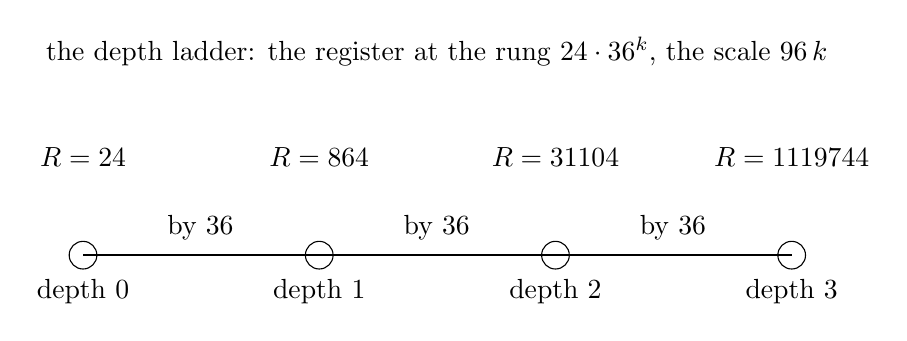
\begin{tikzpicture}[scale=1]
\foreach \x/\k/\r in {0/0/24, 3/1/864, 6/2/31104, 9/3/1119744} {\filldraw[fill=white] (\x,0) circle (5pt) node[below=5pt] {depth $\k$}; \node at (\x,1) [above] {$R = \r$};}
\draw[thick] (0,0) -- (9,0);
\node at (1,0) [above=2pt, xshift=14pt] {by 36}; \node at (4,0) [above=2pt, xshift=14pt] {by 36}; \node at (7,0) [above=2pt, xshift=14pt] {by 36};
\node at (4,2) [above=8pt, xshift=14pt] {the depth ladder: the register at the rung $24\cdot 36^{k}$, the scale $96\,k$};
\end{tikzpicture}\caption{The depth ladder of a chain with the register at each rung; the (3,3) dressing over that register falls by one over thirty-six per rung, the coupling at the depth scale.}\end{figure}
\end{chproof}
\par\medskip\noindent{\itshape The coupling in hand, the next three chapters read the nucleon.}\label{narr:close:7-2}\par
\section{Nucleon structure and the form factor}\label{mod:VII-3-nucleon-structure-and-the-form-factor}
\chdesig{9-3}{7-3}{VII-3-nucleon-structure-and-the-form-factor}{VII-3-nucleon-structure-and-the-form-factor}
\label{narr:open:7-3}Theorem~174.1 reads nucleon structure as the star record census, Theorem~174.2 the junction sharing, the register, the form factor, the office and the pairable legs, and Open result~174.3 the five readings beside.
\begin{chconditional}[Nucleon structure as the star record census]\label{box:VII-3-nucleon-structure-and-the-form-factor:1}
Under its parents, the nucleon of the compendium is a star, a junction qutrit of degree three carrying the three quark bodies of the roster at its leaves, with the docks of the bodies its pendant pairs and the hub of the down body its dressing. The proton star, read link by link at the slot polarity, carries three thousand eight hundred fifty-seven records, each typed at an order and censused at three sets, the docks, the legs and the hub, the fraction of the first-power sum at each set an exact rational, the three summing to one, so the parton structure of the nucleon is a census of the records of its star at their orders: the first-order qutrit-qubit docks read one set, the second-order qutrit-qutrit legs another and the hub a third.
\end{chconditional}
\chstanding{conditional theorem}
\chdeps{Definitions 1.1 to 1.6, Theorems 28.1 and 28.2, Open results 28.3 and 28.4 and Theorem 28.5 and Theorem 171.1 and Open result 171.2}{Open result 175.1, Theorem 175.2 and Open result 175.3, Theorem 176.1 and Open result 176.2, Theorems 177.1 and 177.2 and Open result 177.3, Theorems 181.1 and 181.2 and Open result 181.3 and Theorems 224.1 to 224.3 and Open result 224.4}
The box reads the proton as a small graph and counts, link by link, the records the read engine admits at each link and the order at which it admits them. The three kinds of link carry three disjoint sets of records, and the share of the star's first power that each set carries is an exact fraction.
\begin{chconditional}[The junction sharing, the register, the form factor, the office and the pairable legs]\label{box:VII-3-nucleon-structure-and-the-form-factor:2}
Under their parents, at every one of the 250 junction sites of the roster the flat reduced diagonal of the pair ket at dimension three gives each leg one third of an end, the three thirds summing to one; the register of the nucleon follows from the junction star at the share reading, the proton 85 and the neutron 125; the readout through the star at each of the seven admitted values of the transfer is exact at every one of the twenty-eight cells, so the form factor is an exact object of the star, its size the second transfer sum; the office of the star at the common support is an exact element of the field of root three at each nucleon; and the far set of every junction leg, transported, is a basis of the far support, so no junction leg pairs at a join.
\end{chconditional}
\chstanding{conditional theorems, five}
\chdeps{Definitions 1.1 to 1.6, Theorems 28.1 and 28.2, Open results 28.3 and 28.4 and Theorem 28.5 and Theorem 171.1 and Open result 171.2}{Open result 175.1, Theorem 175.2 and Open result 175.3, Theorem 176.1 and Open result 176.2, Theorems 177.1 and 177.2 and Open result 177.3, Theorems 181.1 and 181.2 and Open result 181.3 and Theorems 224.1 to 224.3 and Open result 224.4}
The second box gathers the five further theorems of the star, how a junction shares its ends among its legs, the register the star reaches, the readout at each admitted transfer, the office, and which legs can pair.
\begin{chwall}[The five readings beside]\label{box:VII-3-nucleon-structure-and-the-form-factor:3}
At every one of the nine lifts the definitions admit, the lifted norm carries the 172 records of the one link to their squared gains not; the local configuration of the electron web at its dock read is not the two-read one-pendant star of the fine-structure derivation; the site product of the located sites equals the first-order star read at the six quark stars but parts from it at both nucleon stars, 201 against 150 at the proton and 963 against 282 at the neutron; the junction star is not the root link opened at both ends; and the end-set selector at the junction face stands as an open result.
\end{chwall}
\chstanding{open results, five, built and not closed}
\chdeps{Definitions 1.1 to 1.6, Theorems 28.1 and 28.2, Open results 28.3 and 28.4 and Theorem 28.5 and Theorem 171.1 and Open result 171.2}{Open result 175.1, Theorem 175.2 and Open result 175.3, Theorem 176.1 and Open result 176.2, Theorems 177.1 and 177.2 and Open result 177.3, Theorems 181.1 and 181.2 and Open result 181.3 and Theorems 224.1 to 224.3 and Open result 224.4}
The third box names the five readings that were tried and parted. The joined Born square at both nucleons stands as a theorem at this chapter.
\begin{chbridge}
What this chapter calls the record census of the star the literature calls the parton structure of the nucleon, the dock set its valence quarks, the leg set its sea and glue, the readout at a transfer its form factor and the register its mass, each the nearest object. The correspondence is by name.
\end{chbridge}
\begin{chproof}[finite computation]
The premises are the read at a register of chapter 1-6, a definition, confinement of chapter 7-1, a theorem, and the framework. The chain from the axiom to this chapter is six chapters long. The procedure. The input is the proton star rebuilt from the cataloged bodies at its leaves, the center a site of dimension 3 with three (3,3) legs to the cores of the leaf bodies, eleven sites of dimensions 3, 3, 3, 3, 2, 2, 2, 4, 2, 2, 2 and eleven links, three legs of genre (3,3), three docks of genre (2,3), one hub leg of genre (3,4), three hub out-legs of genre (2,4) and one pair of genre (2,2), the measure
\begin{equation}
85 = 3 \cdot 9 + 3 \cdot 6 + 12 + 3 \cdot 8 + 4 ;
\end{equation}
the enumeration lists at every link the records of the count law of the read engine, for a passage of center dimension $c$ and far dimension $f$ at the traceless dimensions $A$ and $B$ the roster $4AB + A^{2} + B^{2}$, the swap-fixed $A + B$, the odd sector, the mixed-even sector $2AB$, the same-even sector and the closure, at the gains 1, $f$, $c$ and $cf$. The test types each record at its order. The aggregation censuses the records at the three sets and sums the first power over each. The smallest instance is the dock set, the three (2,3) docks at the first order,
\begin{equation}
516 = 237 + 144 + 126 + 9 ,
\end{equation}
the records by sector, odd, mixed-even, same-even and closure, at the orders 0, 1 and 2 as 237, 270 and 9 and the Born face 957. The three legs at the second order carry 1236 records and the hub a third set, the three together
\begin{equation}
3857
\end{equation}
records of the star.

From the first power at the link measure, the dressing a common factor, by the share of each set, we obtain the fractions at the reading of the first power, the docks 18 over 85, the legs 27 over 85 and the hub 40 over 85, summing to one,
\begin{equation}
\frac{18}{85} + \frac{27}{85} + \frac{40}{85} = 1 ,
\end{equation}
and at the dock-struck reading the docks 0, the legs 27 over 67 and the hub 40 over 67. For the second box the junction gives each leg one third of an end at 250 of 250 junction sites, the register of the proton 85 and the neutron 125 follow at the share reading, the readout at the seven admitted transfers is exact at 28 of 28 cells, the office at the common support is an element of the field of root three at each nucleon, and the far set of every junction leg transported is a basis of the far support.

\emph{Check.} One string of the catalog keying at thirteen of fifteen rows carried three trailing first-power cells inside the closed form at the pinned parse, a fault of the keying and of no cell, re-met at 15 of 15 by a second route and a third. The five counter-tests stand at their pinned letters and the controls the same at both routes with that one repaired. The result was reproduced by an independent route, two engines at every capture byte for byte.
The nuclear norm readout, the star as the electron dock read, the site product at the nucleon stars, the junction star as the root link opened and the end-set selector at the junction face stay open. The proton as a seeded sink is the matter of the next chapter.
\chcert{3857}
\end{chproof}
\begin{figure}[H]\centering
\begin{tikzpicture}[x=0.52pt,y=-0.52pt,baseline]
\clip (0,0) rectangle (900,540);
\fill[white] (0,0) rectangle (900,540);
\node[anchor=base west,inner sep=0pt,text=black,font=\fontsize{6.76}{8.112}\selectfont\ttfamily] at (12,22) {atlas U: U};
\node[anchor=base west,inner sep=0pt,text=black,font=\fontsize{6.24}{7.488}\selectfont\ttfamily] at (12,42) {membership 22:0;23:1;24:0;33:0;34:0;44:0; cells (2,3); links 1; sites 2; measure 6; census at the census};
\node[anchor=base west,inner sep=0pt,text=black,font=\fontsize{5.72}{6.864}\selectfont\ttfamily] at (12,62) {recorded office none; standing census:instrument;nucleon:theorem;roster:roster word; board quark};
\draw[draw=black,line width=1.04pt,dash pattern=on 1.04pt off 1.56pt] (100,250) -- (100,370);
\node[anchor=base,inner sep=0pt,text=black,font=\fontsize{5.72}{6.864}\selectfont\ttfamily] at (100,306) {(2,3)};
\filldraw[fill={rgb,255:red,208;green,208;blue,208},draw=black,line width=0.52pt] (100,250) circle (14);
\node[anchor=base,inner sep=0pt,text=black,font=\fontsize{6.24}{7.488}\selectfont\ttfamily] at (100,255) {3};
\node[anchor=base,inner sep=0pt,text=black,font=\fontsize{5.72}{6.864}\selectfont\ttfamily] at (100,280) {Q};
\filldraw[fill=white,draw=black,line width=0.52pt] (100,370) circle (14);
\node[anchor=base,inner sep=0pt,text=black,font=\fontsize{6.24}{7.488}\selectfont\ttfamily] at (100,375) {2};
\node[anchor=base,inner sep=0pt,text=black,font=\fontsize{5.72}{6.864}\selectfont\ttfamily] at (100,400) {n};
\node[anchor=base west,inner sep=0pt,text=black,font=\fontsize{5.72}{6.864}\selectfont\ttfamily] at (12,510) {the sites labelled by register (2 the qubit, white; 3 the qutrit, grey; 4 the ququart, dark); the links labelled by cell (p,q); a long dash an open dark link of the neutron row; a short dash a docked link at the rule R1};
\end{tikzpicture}
\caption{\texttt{U} (the quark), roster body: 2 sites, 1 links, the measure 6; the links at the cells (2,3); the membership 22:0; 23:1; 24:0; 33:0; 34:0; 44:0; 1 docked links at the rule R1 (Q-n); at the census of the six cells. Drawn at the anatomy atlas as its web, the sites labeled by register and the links by cell, from the nucleon register from the junction star.}\label{fig:VII-3-D520822-u-2e4e97}
\begin{center}\footnotesize\begin{adjustbox}{max width=\linewidth}\begin{tabular}{p{0.26\textwidth}p{0.68\textwidth}}\toprule
recorded office (the slot-count row) & no read of this body at the slot-count row \\
mass register (the mass-register row) & no read of this body at the mass-register row \\
\bottomrule\end{tabular}\end{adjustbox}\end{center}
\end{figure}
\begin{figure}[H]\centering
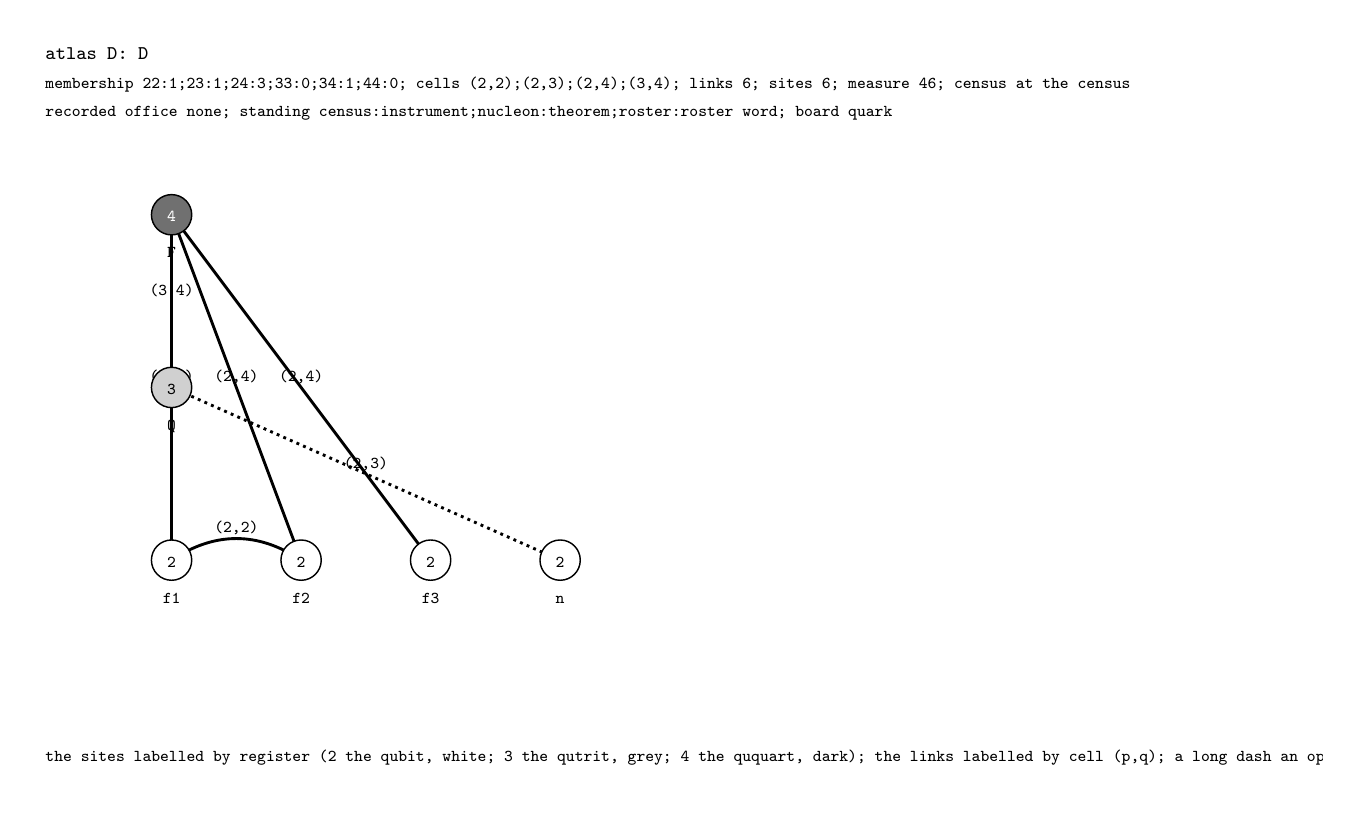
\begin{tikzpicture}[x=0.52pt,y=-0.52pt,baseline]
\clip (0,0) rectangle (900,540);
\fill[white] (0,0) rectangle (900,540);
\node[anchor=base west,inner sep=0pt,text=black,font=\fontsize{6.76}{8.112}\selectfont\ttfamily] at (12,22) {atlas D: D};
\node[anchor=base west,inner sep=0pt,text=black,font=\fontsize{6.24}{7.488}\selectfont\ttfamily] at (12,42) {membership 22:1;23:1;24:3;33:0;34:1;44:0; cells (2,2);(2,3);(2,4);(3,4); links 6; sites 6; measure 46; census at the census};
\node[anchor=base west,inner sep=0pt,text=black,font=\fontsize{5.72}{6.864}\selectfont\ttfamily] at (12,62) {recorded office none; standing census:instrument;nucleon:theorem;roster:roster word; board quark};
\draw[draw=black,line width=1.04pt] (100,130) -- (100,250);
\node[anchor=base,inner sep=0pt,text=black,font=\fontsize{5.72}{6.864}\selectfont\ttfamily] at (100,186) {(3,4)};
\draw[draw=black,line width=1.04pt] (100,130) -- (100,370);
\node[anchor=base,inner sep=0pt,text=black,font=\fontsize{5.72}{6.864}\selectfont\ttfamily] at (100,246) {(2,4)};
\draw[draw=black,line width=1.04pt] (100,130) -- (190,370);
\node[anchor=base,inner sep=0pt,text=black,font=\fontsize{5.72}{6.864}\selectfont\ttfamily] at (145,246) {(2,4)};
\draw[draw=black,line width=1.04pt] (100,130) -- (280,370);
\node[anchor=base,inner sep=0pt,text=black,font=\fontsize{5.72}{6.864}\selectfont\ttfamily] at (190,246) {(2,4)};
\draw[draw=black,line width=1.04pt,dash pattern=on 1.04pt off 1.56pt] (100,250) -- (370,370);
\node[anchor=base,inner sep=0pt,text=black,font=\fontsize{5.72}{6.864}\selectfont\ttfamily] at (235,306) {(2,3)};
\draw[draw=black,line width=1.04pt] (100,370) .. controls (130,350) and (160,350) .. (190,370);
\node[anchor=base,inner sep=0pt,text=black,font=\fontsize{5.72}{6.864}\selectfont\ttfamily] at (145,351) {(2,2)};
\filldraw[fill={rgb,255:red,112;green,112;blue,112},draw=black,line width=0.52pt] (100,130) circle (14);
\node[anchor=base,inner sep=0pt,text=white,font=\fontsize{6.24}{7.488}\selectfont\ttfamily] at (100,135) {4};
\node[anchor=base,inner sep=0pt,text=black,font=\fontsize{5.72}{6.864}\selectfont\ttfamily] at (100,160) {F};
\filldraw[fill={rgb,255:red,208;green,208;blue,208},draw=black,line width=0.52pt] (100,250) circle (14);
\node[anchor=base,inner sep=0pt,text=black,font=\fontsize{6.24}{7.488}\selectfont\ttfamily] at (100,255) {3};
\node[anchor=base,inner sep=0pt,text=black,font=\fontsize{5.72}{6.864}\selectfont\ttfamily] at (100,280) {Q};
\filldraw[fill=white,draw=black,line width=0.52pt] (100,370) circle (14);
\node[anchor=base,inner sep=0pt,text=black,font=\fontsize{6.24}{7.488}\selectfont\ttfamily] at (100,375) {2};
\node[anchor=base,inner sep=0pt,text=black,font=\fontsize{5.72}{6.864}\selectfont\ttfamily] at (100,400) {f1};
\filldraw[fill=white,draw=black,line width=0.52pt] (190,370) circle (14);
\node[anchor=base,inner sep=0pt,text=black,font=\fontsize{6.24}{7.488}\selectfont\ttfamily] at (190,375) {2};
\node[anchor=base,inner sep=0pt,text=black,font=\fontsize{5.72}{6.864}\selectfont\ttfamily] at (190,400) {f2};
\filldraw[fill=white,draw=black,line width=0.52pt] (280,370) circle (14);
\node[anchor=base,inner sep=0pt,text=black,font=\fontsize{6.24}{7.488}\selectfont\ttfamily] at (280,375) {2};
\node[anchor=base,inner sep=0pt,text=black,font=\fontsize{5.72}{6.864}\selectfont\ttfamily] at (280,400) {f3};
\filldraw[fill=white,draw=black,line width=0.52pt] (370,370) circle (14);
\node[anchor=base,inner sep=0pt,text=black,font=\fontsize{6.24}{7.488}\selectfont\ttfamily] at (370,375) {2};
\node[anchor=base,inner sep=0pt,text=black,font=\fontsize{5.72}{6.864}\selectfont\ttfamily] at (370,400) {n};
\node[anchor=base west,inner sep=0pt,text=black,font=\fontsize{5.72}{6.864}\selectfont\ttfamily] at (12,510) {the sites labelled by register (2 the qubit, white; 3 the qutrit, grey; 4 the ququart, dark); the links labelled by cell (p,q); a long dash an open dark link of the neutron row; a short dash a docked link at the rule R1};
\end{tikzpicture}
\caption{\texttt{D} (the quark), roster body: 6 sites, 6 links, the measure 46; the links at the cells (2,2), (2,3), (2,4), (3,4); the membership 22:1; 23:1; 24:3; 33:0; 34:1; 44:0; 1 docked links at the rule R1 (Q-n); at the census of the six cells. Drawn at the anatomy atlas as its web, the sites labeled by register and the links by cell, from the nucleon register from the junction star.}\label{fig:VII-3-D520822-d-8c290a}
\begin{center}\footnotesize\begin{adjustbox}{max width=\linewidth}\begin{tabular}{p{0.26\textwidth}p{0.68\textwidth}}\toprule
recorded office (the slot-count row) & no read of this body at the slot-count row \\
mass register (the mass-register row) & no read of this body at the mass-register row \\
\bottomrule\end{tabular}\end{adjustbox}\end{center}
\end{figure}
\label{chend:VII-3-nucleon-structure-and-the-form-factor}
\par\medskip\noindent{\itshape The structure read, the next chapter builds the proton as a sink.}\label{narr:close:7-3}\par
\section{The proton as a seeded sink}\label{mod:VII-4-proton-as-a-seeded-sink}
\chdesig{9-4}{7-4}{VII-4-proton-as-a-seeded-sink}{VII-4-proton-as-a-seeded-sink}
\label{narr:open:7-4}Open result~175.1 states the seeded saturation of the proton web, Theorem~175.2 the joined read at the roster stars, Open result~175.3 the six readings beside, and Open result~175.4 the cap census at the proton sinks.
\begin{chwall}[The seeded saturation of the proton web]\label{box:VII-4-proton-as-a-seeded-sink:1}
The proton seed, the hub-attached three-quark web at the star core with the pair hub, ten sites and twelve links, is its own sink at wave zero at the stop condition of the pairing move, so that the saturation of the proton seed under that move is the seed itself, while under the twenty-eight catalogued moves the closure grows to twenty-five thousand five hundred fifty-eight webs at wave four, unstopped at the candidate bound. On the one face the seed is a sink at wave zero with the first power 2727 at the hub spelling and 101 at the dock spelling; on the other face the saturation is unstopped at the bound and the candidate cell 8613 equals the first power at no sink of the bounded closure at any reading, the parting named with both objects, 2727 against 8613. Re-posed with the budget replaced by the site bound six of the closure without caps: the proton seed stands at ten sites beyond the bound, so the first chain reaching the bound is the seed itself at wave zero, a chain of length zero and its own sink, every one of its fifteen candidates under the twenty-eight moves refused at the bound at wave one, the closure the seed alone and exhausted at wave zero with no web within the bound and one beyond, the bound reached without a sink named within it; at the site bounds ten, eleven and twelve beside the closure stops at one, two and three webs with the seed its own sink at every reading, the first power 2727 at the hub spelling and 101 at the dock spelling re-met, and the sinks of this saturation at the site bands ten to twelve share no band with the forty-one forward sinks of the closure without caps at the bands three to six, so the two closures meet at no state by site count.
\end{chwall}
\chstanding{open result, built and not closed}
\chdeps{Definitions 1.1 to 1.6, Theorem 171.1 and Open result 171.2, Theorems 174.1 and 174.2 and Open result 174.3 and Open results 245.1 and 245.2, Theorem 245.3, Open results 245.4 to 245.8 and Theorem 245.9}{Open result 175.4 and Theorem 176.1 and Open result 176.2}
The box follows the proton as the thing the saturation of a seed reaches, which is not the roster star of the previous chapter but a web that grows from it. Under the one pairing move the seed is already stable, and under every move the growth does not stop inside the bound.
\begin{chconditional}[The joined read at the roster stars]\label{box:VII-4-proton-as-a-seeded-sink:2}
Under its parents, the roster stars of the proton and the neutron, each joined at the dock to the measurement web of its row, give the direct record sum to order three at the dock unit, every order exact and signed and the order-three term zero at every reading.
\end{chconditional}
\chstanding{conditional theorem}
\chdeps{Definitions 1.1 to 1.6, Theorem 171.1 and Open result 171.2, Theorems 174.1 and 174.2 and Open result 174.3 and Open results 245.1 and 245.2, Theorem 245.3, Open results 245.4 to 245.8 and Theorem 245.9}{Open result 175.4 and Theorem 176.1 and Open result 176.2}
The second box is the one theorem of the chapter, the roster star joined to its measuring web has an exact direct sum order by order.
\begin{chwall}[The six readings beside]\label{box:VII-4-proton-as-a-seeded-sink:3}
The one-link records weighted by the states they reach at the open ends of the star sum to 319, the both-ends Born count of the support-rank entry by construction, the identity of a count with itself and no reach; no sink of the site-bounded closure, 44341 sinks at wave four, and no sink of the clean twin reads the proton figure of the comparison table at any reading tried, so the candidate is refuted at the bounded closures; the first catalogued proton sink, eight sites and nine links at the unstruck measure 81, reads 2187 at the hub spelling of the measure law, equal at none of twelve readings to the figure of the proton row, the exact ratio 319 over 81; at the proton sink the three coloured junction legs are the open interior links of the confinement theorem, and the Born count over their open end sets is 3108, parting from the catalogued figure cell as an exact integer identity; the register grows from the seed to the saturated proton by the factor one, so the running at that growth is zero; and the proton sink record spectrum with no frame stands as an open result.
\end{chwall}
\chstanding{open results, six, built and not closed}
\chdeps{Definitions 1.1 to 1.6, Theorem 171.1 and Open result 171.2, Theorems 174.1 and 174.2 and Open result 174.3 and Open results 245.1 and 245.2, Theorem 245.3, Open results 245.4 to 245.8 and Theorem 245.9}{Open result 175.4 and Theorem 176.1 and Open result 176.2}
The third box names the readings of the proton as a sink that were tried and parted, every one leaving the proton row of the comparison table outside the comparison. The strong coupling at the junction of the saturated proton stands as a theorem at this chapter.
\begin{chbridge}
What this chapter calls the proton seed and its sink the literature calls the proton, the pairing move its binding and the first power at the sink its mass. The correspondence is by name, and the proton row of the comparison table stands outside the comparison at every reading produced.
\end{chbridge}
\begin{chproof}[finite computation]
The premises are the saturation with its seeds, waves and sinks of chapter 1-5, a theorem, confinement of chapter 7-1 and the nucleon star of chapter 7-3, theorems. The chain from the axiom to this chapter is seven chapters long. The procedure. The input is the proton seed, the hub-attached block of the star core and the pair hub, the center $J$ with a (3,3) leg to each quark, an up dock at each quark, the hub $H$ with a (3,4) leg from each quark and the pair, ten sites and twelve links, the measure
\begin{equation}
101 = 3 \cdot 9 + 3 \cdot 6 + 3 \cdot 12 + 2 \cdot 8 + 4 ,
\end{equation}
three in-legs at the hub rule and the hub beyond the valence bound at degree 5. The enumeration grows the closure from the seed wave by wave under the moves, every intermediate web printed at its measure, its unstruck measure, its in-leg count and its first powers. The test at every web is the stop condition, no closed-equal site with spare and the pairing move admitting no join. The aggregation counts the sinks by wave. The smallest instance is the seed itself, a sink at wave zero, with the first power at the hub spelling the unstruck measure multiplied by three to the in-legs and at the dock spelling the measure,
\begin{equation}
2727 = 101 \cdot 3^{3}, \qquad 101 ,
\end{equation}
and the display over the electron cell squared, $826281/4489$, compared with nothing here.

Under the pairing move alone the seed is the whole closure, stopped and exhausted at wave one. Under the twenty-eight moves the closure grows as
\begin{equation}
25558 = 1 + 12 + 252 + 7297 + 17996
\end{equation}
over the waves zero to four, unstopped at the candidate bound at the first slice of wave four, with 16946 sinks at the stop condition, by wave 1, 10, 170, 4249 and 12516. The neutron reading, the seed with one arm turned down, is its own sink alike with the first power 10773 at the hub spelling and 133 at the dock spelling, the additive difference from the proton 32 at the dock spelling and 8046 at the hub. The control, the cataloged electron as a seed, is its own sink at wave zero and re-meets its first power 201 and 67 at the readings striking the docks. The candidate cell 8613 equals the first power at no sink of the bounded closure at any reading, the parting of the box.

\emph{Check.} The self-loop count read zero at every wave of every closure. The electron control parts at the readings striking no dock, 237 and 79, and meets at the others. The result was reproduced by an independent route, two engines at every capture byte for byte, its four counter-tests at their pinned letters and its eleven controls the same at both routes.
The proton as a sink of the saturation stays open at every reading, the seeded saturation unstopped or parting, the first power at the sink no integer reading of the proton row, and the open count, the register growth and the record spectrum at their partings.
\chcert{25558}
\end{chproof}
\label{chend:VII-4-proton-as-a-seeded-sink}
\subsection{The cap census at the proton sinks}\label{mod:VII-4-D535254-w-prca}
\begin{chwall}[The cap census at the proton sinks]\label{box:VII-4-D535254-w-prca:1}
At every link of every proton sink of the roster census, seven webs at 80 links with 19 open docks, the record count at the primary map reading equals the cap of its genre at all 80 links, so every link is capped at the adopted typing, the coloured links capped at all 22 and the cap of every roster web met again at all seven, the 228 link-end caps at their genre cells. On the one face every link is capped; on the other face the readout of the first sink parts from the candidate and seed cells at both leg readings, 25839 at the counted reading and 8613 at the excluded reading against the cells 2871 and 2727, the parting named with both cells.
\end{chwall}
\chstanding{open result, built and not closed}
\chdeps{Definitions 1.1 to 1.6 and Open result 175.1, Theorem 175.2 and Open result 175.3}{no theorem beyond it at this release}
The box checks that every link of every proton-like stable web already carries as many records as its genre allows, and then asks whether the readout principle applied to such a capped web reproduces the two proton cells of the construction. It does not at either.
\begin{chbridge}
What this chapter calls the cap of a genre the literature calls the dimension of the record space of a link, the nearest object. The correspondence is by name, and the counts of this chapter are exact objects compared with nothing here.
\end{chbridge}
\begin{chproof}[finite computation]
The premises are the proton chapter above and the framework. The chain from the axiom to this result is eight chapters long. The procedure. The input is the roster of seven webs, the bound-respecting seed sink, the proton-web seed sink, the star-face sink and the cataloged star beside, the neutron twin and the two electron controls, at 80 links and 19 open docks. The enumeration lists every link with its genre and the record count at the map reading. The test compares the count with the cap of the genre, the Born count. The aggregation counts the capped and open links. The result is capped at 80 of 80 and open at 0 of 80, the first uncapped link none, the colored links capped at 22 of 22, the open-end links by the adopted definition of open 51 of 80 beside, and the caps of the seven webs and the 228 link-end caps re-met at their genre cells,
\begin{equation}
80 = 80 + 0, \qquad 22 = 22 + 0 .
\end{equation}
The smallest instance of the second face is the first sink, its readout at the principle, every open dock adding the Born count of the dock genre, reads 25839 at the counted reading and 8613 at the excluded reading at the dressings 27 and 9, against the candidate cell 2871 and the seed cell 2727,
\begin{equation}
25839 = 9 \cdot 2871, \qquad 8613 = 3 \cdot 2871, \qquad 8613 \neq 2727 ,
\end{equation}
parting at both leg readings, the one-dock reading beside equal at 2 of 2.

From the eleven comparisons against the dock numerators, by the same steps, the star-face sink equals the candidate at both readings and parts from the seed, and the two cataloged proton sinks equal at one leg reading at 0 of 2. The dressing equals the far-end cell of the parent at 4 of 4 webs carrying one.

\emph{Check.} The typed rows of every consumed table were counted at their records and apart. The comparisons stand at the exact integer differences and reduced ratios of the table. The result was reproduced by an independent route, two engines at every capture byte for byte, its counter-tests at their pinned letters and its controls the same at both routes.
The proton figure as the readout of a capped web stays equal at neither cataloged proton sink.
\chcert{80}
\end{chproof}
\label{chend:VII-4-D535254-w-prca}
\par\medskip\noindent{\itshape The proton built, the next chapter reads the ratio of its mass to the mass of the electron.}\label{narr:close:7-4}\par
\section{The proton-to-electron ratio: a candidate}\label{mod:VII-5-proton-to-electron-ratio-a-candidate}
\chdesig{9-5}{7-5}{VII-5-proton-to-electron-ratio-a-candidate}{VII-5-proton-to-electron-ratio-a-candidate}
\label{narr:open:7-5}Theorem~176.1 reads the mass ratio at the second-order read, a candidate stated as a candidate, with the six readings beside in Open result~176.2.
\begin{chconditional}[The mass ratio at the second-order read]\label{box:VII-5-proton-to-electron-ratio-a-candidate:1}
Under its parents, the lepton bodies are met again, the order of the read is exact, the ratio at the second-order read is exact and the Koide object is exact: the charged-lepton ratios at the second order of the read are exact objects compared at the direct reading of the comparison table, and this compendium displays them nowhere. The proton in the electron unit stands outside the comparison by orders at every reading the construction has produced, the object at those readings of another kind than the measured ratio as the comparison table types it.
\end{chconditional}
\chstanding{conditional theorem}
\chdeps{Definitions 1.1 to 1.6, Theorems 9.1 to 9.7 and Open result 9.8, Theorems 18.1 to 18.4 and Open results 18.5 and 18.6, Theorems 174.1 and 174.2 and Open result 174.3 and Open result 175.1, Theorem 175.2 and Open result 175.3}{no theorem beyond it at this release}
The box reads the three charged leptons at the second order of the read engine and forms their ratios and the Koide combination as exact numbers of the field. What it says about the proton is only that no reading yet produced lands the proton in the electron unit at the kind the comparison table asks.
\begin{chwall}[The six readings beside]\label{box:VII-5-proton-to-electron-ratio-a-candidate:2}
The two ticks are exact and their squared ratio is two at the adopted unit, but the one unit tying the lattice step of the order register to the Killing norm of a direction step is fixed by no result of this work; the support rank of the one qutrit-qubit link is the Born count over both ends, 319 as the sum over the 172 record letters, but the act readout sum of a roster web reading the link through its open qubit end is not that count at any catalogued web, the electron at its dock-struck rank 67 against 350; the 79 closed records of the one link fall into 48 mixed records, 28 at two qutrit slots and 3 at two qubit slots, and no union of these sets stands at 27, 40 or 12, the weights of the three sets of the roster electron, so the electron is forced at no partition of the closed records; the sinks of the bare link, the ladder at the hadron rows and the leg count from the end set each stand as an open result at their partings; the mass ratios at the one readout stand at this chapter.
\end{chwall}
\chstanding{open results, six, built and not closed}
\chdeps{Definitions 1.1 to 1.6, Theorems 9.1 to 9.7 and Open result 9.8, Theorems 18.1 to 18.4 and Open results 18.5 and 18.6, Theorems 174.1 and 174.2 and Open result 174.3 and Open result 175.1, Theorem 175.2 and Open result 175.3}{no theorem beyond it at this release}
The second box names the readings that would carry the candidate and part.
\begin{chbridge}
What this chapter calls the ratio at the second-order read the literature calls the ratio of two lepton masses and the Koide object the Koide combination, the nearest objects. The correspondence is by name, and this chapter displays no measured value.
\end{chbridge}
\begin{chproof}[exact]
The premises are the link and its six genres of chapter 1-2 and the reads and the Born count of chapter 1-3, definitions, the nucleon star of chapter 7-3 and the proton sink of chapter 7-4, the chain from the axiom eight chapters long. The set counted is the reads of the three charged-lepton bodies at the second order of the read engine, 1972 cells over the links at the three faces, the port of the construction, the struck links summed and the dark-port face, and the property tested is the exactness of the second-order term at each link, the first-order term multiplied by the square of the second-order readout. The exact part. From the first powers of the three bodies, the dock-struck rank multiplied by the hub dressing, we obtain at the first order the ratios
\begin{equation}
\frac{S_\mu}{S_e} = \frac{963}{201}, \qquad \Bigl(\frac{963}{201}\Bigr)^{2} = \frac{103041}{4489}, \qquad \Bigl(\frac{3969}{201}\Bigr)^{2} = \frac{1750329}{4489},
\end{equation}
the muon and the tau over the electron, equal to the earlier result at 2 of 2. From the electron at its port, the (2,3) link at the cut-register star 20736, by the second-order readout, we obtain
\begin{equation}
G_{2} = \frac{79}{20736} + \frac{1}{432}\sqrt{2} + \frac{7}{3456}\sqrt{3} + \frac{1}{6912}\sqrt{6} ,
\end{equation}
and the second-order term $T_{1} G_{2}^{2}$, nonzero, the mass at the first plus second order $T_{1}(1 + G_{2}^{2})$. At the port of the construction the muon-to-electron ratio keeps $103041/4489$ with the relative second-order part zero, the two bodies entering at a (2,3) port carrying one $G_{2}$ each. The Koide combination at the first order, the sum of the three masses over the square of the sum of their roots, the roots the first-power ratios with the sum $5133/67$ and the sum of squares $16720731/4489$, is
\begin{equation}
\frac{1857859}{2927521} = \frac{2}{3} - \frac{281465}{8782563} ,
\end{equation}
its departure from two thirds nonzero and exact.
\end{chproof}
\begin{chproof}[census]
The census part. By kind the second-order terms are nonzero at every link of the three bodies at the three faces, exact elements of the field at every cell, the three masses equal as rationals at 3 of 3 at the unit spelled as one, the smallest case the electron at its one port, the display above. The proton in the electron unit stands outside the comparison by orders at every reading produced.

\emph{Check.} Two keyings of the pinned engines, the unit mass spelled 1 against 1 over 1 and a histogram counted over the change table in place of the typing table, parted at one part of ten and one of eleven, every cell equal at a second route and a third with the keyings re-met. The Koide object at the first plus second order stands at the table of the entry as a rational of more than a hundred digits, and the result was reproduced by an independent route, two engines at every capture byte for byte, its counter-tests at their pinned letters.
\chcert{1972}
\end{chproof}
\label{chend:VII-5-proton-to-electron-ratio-a-candidate}
\par\medskip\noindent{\itshape From one hadron the thread widens to the whole spectrum.}\label{narr:close:7-5}\par
\section{The hadron spectrum and the mesons}\label{mod:VII-6-hadron-spectrum-and-the-mesons}
\chdesig{9-6}{7-6}{VII-6-hadron-spectrum-and-the-mesons}{VII-6-D543708-w-hdom}
\label{narr:open:7-6}Theorem~177.1 reads the hadron spectrum as the roster of saturated joined webs, Theorem~177.2 the mixed composition, the meson apparatus and the corollaries, and Open result~177.3 the direct sum at the deuteron as an open result.
\begin{chconditional}[The hadron spectrum as the roster of saturated joined webs]\label{box:VII-6-hadron-spectrum-and-the-mesons:1}
Under its parents, at the pairable set of the nucleon star, two docks at the proton star and one at the neutron star, the pairing move builds, up to four stars, exactly the joined webs admitted, and its sinks are exactly the saturated webs found: the chains of two neutron stars, of a proton between two neutrons and of two protons between two neutrons, the proton cycles of three and of four, the triton and the web of two neutrons and two protons, the deuteron never; beyond four stars the spectrum is the chain of proton stars capped by two neutron stars and the cycle of proton stars at every star count from five to the bound eight, two new sinks at every count, fourteen webs in all, each at the register 16 at the dock face and 81 at the port face.
\begin{figure}[H]\centering
\begin{adjustbox}{max width=\linewidth}\begin{tikzpicture}[x=0.52pt,y=-0.52pt,baseline]
\clip (0,0) rectangle (900,540);
\fill[white] (0,0) rectangle (900,540);
\node[anchor=base west,inner sep=0pt,text=black,font=\fontsize{6.76}{8.112}\selectfont\ttfamily] at (12,22) {atlas u\_docked: u\_docked};
\node[anchor=base west,inner sep=0pt,text=black,font=\fontsize{6.24}{7.488}\selectfont\ttfamily] at (12,42) {membership 22:0;23:2;24:0;33:0;34:0;44:0; cells (2,3); links 2; sites 3; measure 12; census at the census};
\node[anchor=base west,inner sep=0pt,text=black,font=\fontsize{5.72}{6.864}\selectfont\ttfamily] at (12,62) {recorded office none; standing census:instrument;hadron:open result;quark:open result;roster:roster word; board quark};
\draw[draw=black,line width=1.04pt,dash pattern=on 1.04pt off 1.56pt] (100,370) -- (100,250);
\node[anchor=base,inner sep=0pt,text=black,font=\fontsize{5.72}{6.864}\selectfont\ttfamily] at (100,306) {(2,3)};
\draw[draw=black,line width=1.04pt,dash pattern=on 1.04pt off 1.56pt] (100,250) -- (190,370);
\node[anchor=base,inner sep=0pt,text=black,font=\fontsize{5.72}{6.864}\selectfont\ttfamily] at (145,306) {(2,3)};
\filldraw[fill=white,draw=black,line width=0.52pt] (100,370) circle (14);
\node[anchor=base,inner sep=0pt,text=black,font=\fontsize{6.24}{7.488}\selectfont\ttfamily] at (100,375) {2};
\node[anchor=base,inner sep=0pt,text=black,font=\fontsize{5.72}{6.864}\selectfont\ttfamily] at (100,400) {Jd};
\filldraw[fill={rgb,255:red,208;green,208;blue,208},draw=black,line width=0.52pt] (100,250) circle (14);
\node[anchor=base,inner sep=0pt,text=black,font=\fontsize{6.24}{7.488}\selectfont\ttfamily] at (100,255) {3};
\node[anchor=base,inner sep=0pt,text=black,font=\fontsize{5.72}{6.864}\selectfont\ttfamily] at (100,280) {Q};
\filldraw[fill=white,draw=black,line width=0.52pt] (190,370) circle (14);
\node[anchor=base,inner sep=0pt,text=black,font=\fontsize{6.24}{7.488}\selectfont\ttfamily] at (190,375) {2};
\node[anchor=base,inner sep=0pt,text=black,font=\fontsize{5.72}{6.864}\selectfont\ttfamily] at (190,400) {n};
\node[anchor=base west,inner sep=0pt,text=black,font=\fontsize{5.72}{6.864}\selectfont\ttfamily] at (12,510) {the sites labelled by register (2 the qubit, white; 3 the qutrit, grey; 4 the ququart, dark); the links labelled by cell (p,q); a long dash an open dark link of the neutron row; a short dash a docked link at the rule R1};
\end{tikzpicture}\end{adjustbox}
\caption{\texttt{u\_docked} (the quark), hadron row body: 3 sites, 2 links, the measure 12; the links at the cells (2,3); the membership 22:0; 23:2; 24:0; 33:0; 34:0; 44:0; 2 docked links at the rule R1 (Q-n; Q-Jd); at the census of the six cells. Drawn at the anatomy atlas as its web, the sites labeled by register and the links by cell, from the hadron spectroscopy at the cap sinks.}\label{fig:VII-6-D540002-u-docked-e37fe0}
\begin{center}\footnotesize\begin{adjustbox}{max width=\linewidth}\begin{tabular}{p{0.26\textwidth}p{0.68\textwidth}}\toprule
recorded office (the slot-count row) & no read of this body at the slot-count row \\
mass register (the mass-register row) & the read KU: the class within the qubit and the qutrit; the first power 0; the office \texttt{0\textbar{}0\textbar{}0\textbar{}0}; zero; met yes; hubs none; in-legs none; dressing 1; ports Q-n; Q-Jd \\
\bottomrule\end{tabular}\end{adjustbox}\end{center}
\end{figure}
\begin{figure}[H]\centering
\begin{adjustbox}{max width=\linewidth}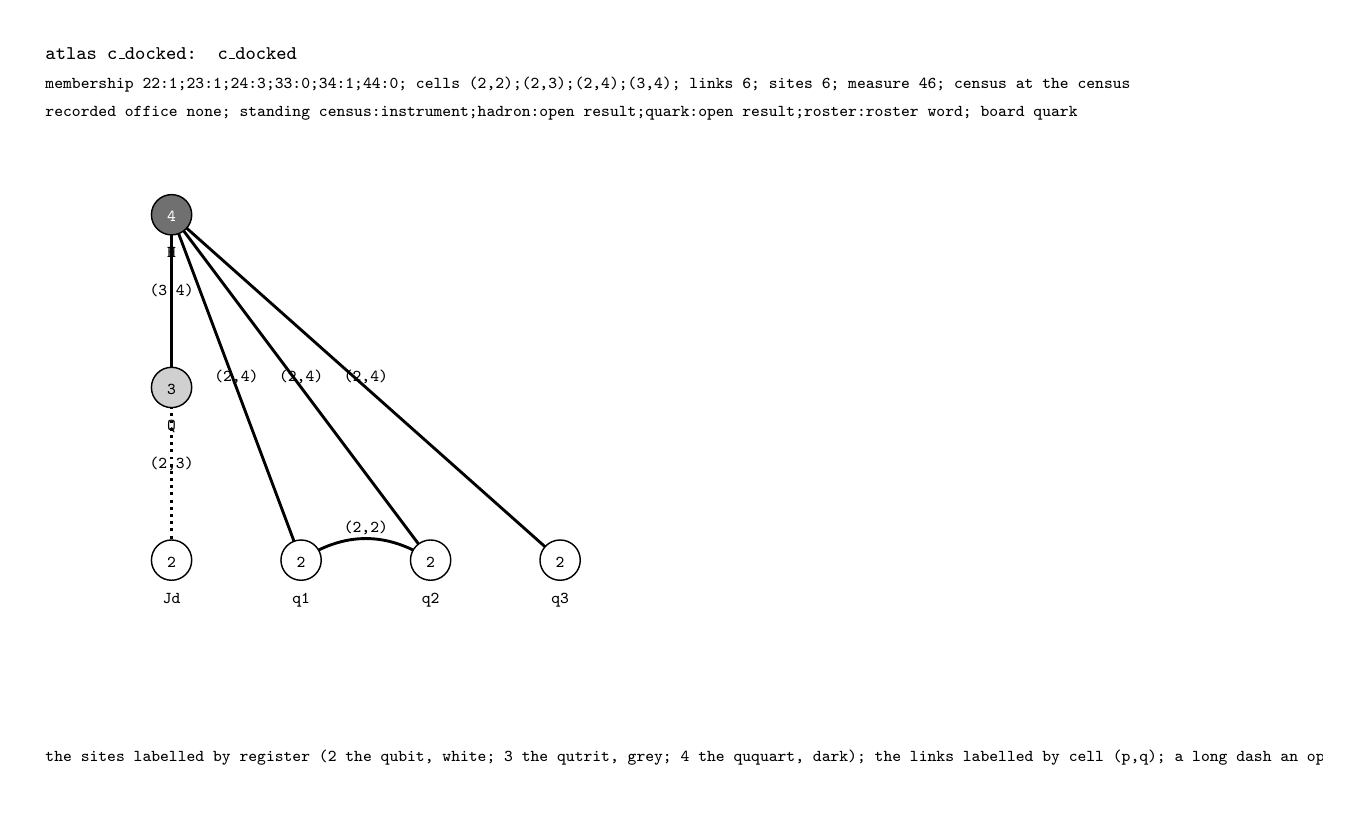
\begin{tikzpicture}[x=0.52pt,y=-0.52pt,baseline]
\clip (0,0) rectangle (900,540);
\fill[white] (0,0) rectangle (900,540);
\node[anchor=base west,inner sep=0pt,text=black,font=\fontsize{6.76}{8.112}\selectfont\ttfamily] at (12,22) {atlas c\_docked: c\_docked};
\node[anchor=base west,inner sep=0pt,text=black,font=\fontsize{6.24}{7.488}\selectfont\ttfamily] at (12,42) {membership 22:1;23:1;24:3;33:0;34:1;44:0; cells (2,2);(2,3);(2,4);(3,4); links 6; sites 6; measure 46; census at the census};
\node[anchor=base west,inner sep=0pt,text=black,font=\fontsize{5.72}{6.864}\selectfont\ttfamily] at (12,62) {recorded office none; standing census:instrument;hadron:open result;quark:open result;roster:roster word; board quark};
\draw[draw=black,line width=1.04pt] (100,130) -- (100,250);
\node[anchor=base,inner sep=0pt,text=black,font=\fontsize{5.72}{6.864}\selectfont\ttfamily] at (100,186) {(3,4)};
\draw[draw=black,line width=1.04pt] (100,130) -- (190,370);
\node[anchor=base,inner sep=0pt,text=black,font=\fontsize{5.72}{6.864}\selectfont\ttfamily] at (145,246) {(2,4)};
\draw[draw=black,line width=1.04pt] (100,130) -- (280,370);
\node[anchor=base,inner sep=0pt,text=black,font=\fontsize{5.72}{6.864}\selectfont\ttfamily] at (190,246) {(2,4)};
\draw[draw=black,line width=1.04pt] (100,130) -- (370,370);
\node[anchor=base,inner sep=0pt,text=black,font=\fontsize{5.72}{6.864}\selectfont\ttfamily] at (235,246) {(2,4)};
\draw[draw=black,line width=1.04pt,dash pattern=on 1.04pt off 1.56pt] (100,370) -- (100,250);
\node[anchor=base,inner sep=0pt,text=black,font=\fontsize{5.72}{6.864}\selectfont\ttfamily] at (100,306) {(2,3)};
\draw[draw=black,line width=1.04pt] (190,370) .. controls (220,350) and (250,350) .. (280,370);
\node[anchor=base,inner sep=0pt,text=black,font=\fontsize{5.72}{6.864}\selectfont\ttfamily] at (235,351) {(2,2)};
\filldraw[fill={rgb,255:red,112;green,112;blue,112},draw=black,line width=0.52pt] (100,130) circle (14);
\node[anchor=base,inner sep=0pt,text=white,font=\fontsize{6.24}{7.488}\selectfont\ttfamily] at (100,135) {4};
\node[anchor=base,inner sep=0pt,text=black,font=\fontsize{5.72}{6.864}\selectfont\ttfamily] at (100,160) {H};
\filldraw[fill=white,draw=black,line width=0.52pt] (100,370) circle (14);
\node[anchor=base,inner sep=0pt,text=black,font=\fontsize{6.24}{7.488}\selectfont\ttfamily] at (100,375) {2};
\node[anchor=base,inner sep=0pt,text=black,font=\fontsize{5.72}{6.864}\selectfont\ttfamily] at (100,400) {Jd};
\filldraw[fill={rgb,255:red,208;green,208;blue,208},draw=black,line width=0.52pt] (100,250) circle (14);
\node[anchor=base,inner sep=0pt,text=black,font=\fontsize{6.24}{7.488}\selectfont\ttfamily] at (100,255) {3};
\node[anchor=base,inner sep=0pt,text=black,font=\fontsize{5.72}{6.864}\selectfont\ttfamily] at (100,280) {Q};
\filldraw[fill=white,draw=black,line width=0.52pt] (190,370) circle (14);
\node[anchor=base,inner sep=0pt,text=black,font=\fontsize{6.24}{7.488}\selectfont\ttfamily] at (190,375) {2};
\node[anchor=base,inner sep=0pt,text=black,font=\fontsize{5.72}{6.864}\selectfont\ttfamily] at (190,400) {q1};
\filldraw[fill=white,draw=black,line width=0.52pt] (280,370) circle (14);
\node[anchor=base,inner sep=0pt,text=black,font=\fontsize{6.24}{7.488}\selectfont\ttfamily] at (280,375) {2};
\node[anchor=base,inner sep=0pt,text=black,font=\fontsize{5.72}{6.864}\selectfont\ttfamily] at (280,400) {q2};
\filldraw[fill=white,draw=black,line width=0.52pt] (370,370) circle (14);
\node[anchor=base,inner sep=0pt,text=black,font=\fontsize{6.24}{7.488}\selectfont\ttfamily] at (370,375) {2};
\node[anchor=base,inner sep=0pt,text=black,font=\fontsize{5.72}{6.864}\selectfont\ttfamily] at (370,400) {q3};
\node[anchor=base west,inner sep=0pt,text=black,font=\fontsize{5.72}{6.864}\selectfont\ttfamily] at (12,510) {the sites labelled by register (2 the qubit, white; 3 the qutrit, grey; 4 the ququart, dark); the links labelled by cell (p,q); a long dash an open dark link of the neutron row; a short dash a docked link at the rule R1};
\end{tikzpicture}\end{adjustbox}
\caption{\texttt{c\_docked} (the quark), hadron row body: 6 sites, 6 links, the measure 46; the links at the cells (2,2), (2,3), (2,4), (3,4); the membership 22:1; 23:1; 24:3; 33:0; 34:1; 44:0; 1 docked links at the rule R1 (Q-Jd); at the census of the six cells. Drawn at the anatomy atlas as its web, the sites labeled by register and the links by cell, from the hadron spectroscopy at the cap sinks.}\label{fig:VII-6-D540002-c-docked-e456cf}
\begin{center}\footnotesize\begin{adjustbox}{max width=\linewidth}\begin{tabular}{p{0.26\textwidth}p{0.68\textwidth}}\toprule
recorded office (the slot-count row) & no read of this body at the slot-count row \\
mass register (the mass-register row) & the read KC: the class touching the ququart; the first power 120; the office \texttt{47776588143529/3317760000\textbar{}661/4050\textbar{}5069/41472000\textbar{}0}; nonzero; met yes; hubs H; in-legs q-h; dressing 3; ports H-q3; Q-Jd \\
\bottomrule\end{tabular}\end{adjustbox}\end{center}
\end{figure}
\begin{figure}[H]\centering
\begin{adjustbox}{max width=\linewidth}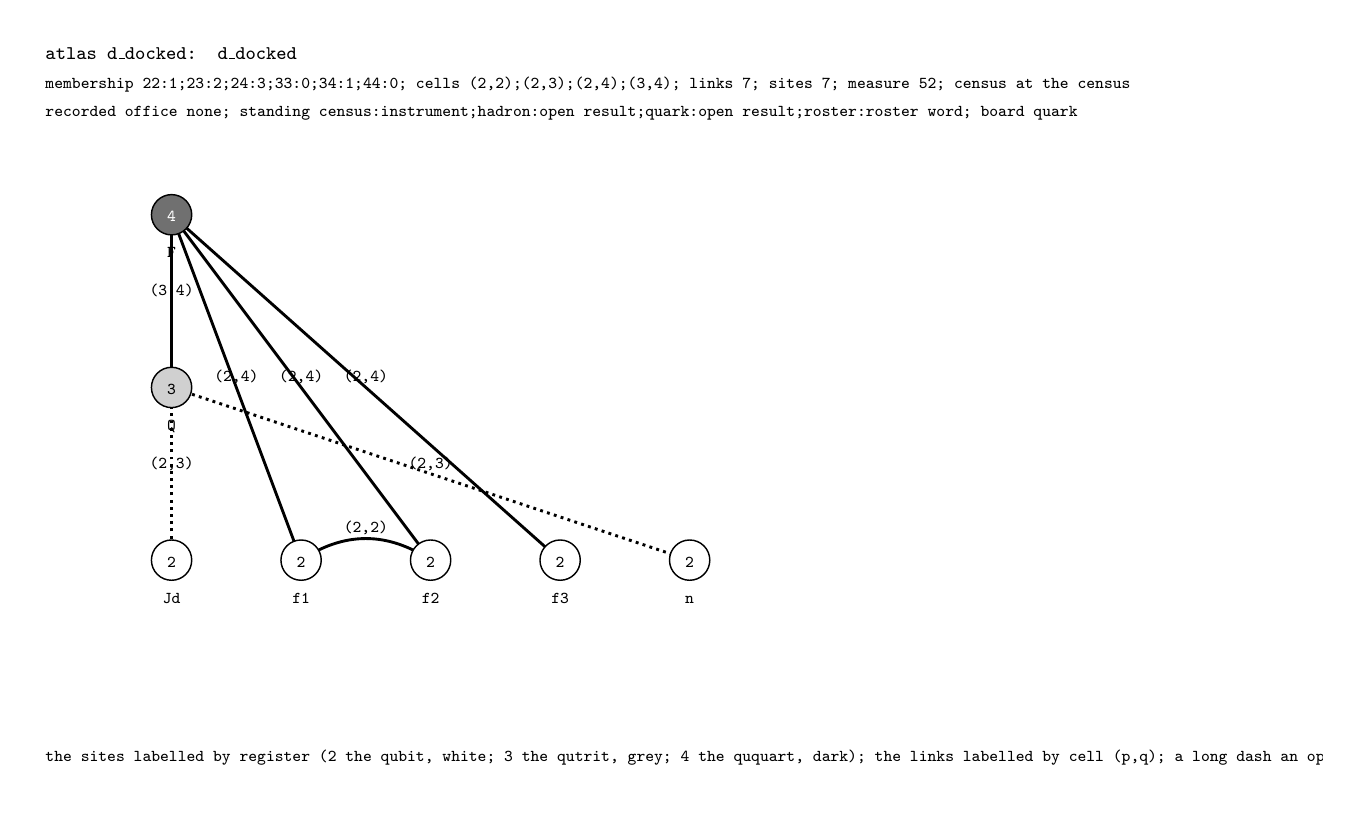
\begin{tikzpicture}[x=0.52pt,y=-0.52pt,baseline]
\clip (0,0) rectangle (900,540);
\fill[white] (0,0) rectangle (900,540);
\node[anchor=base west,inner sep=0pt,text=black,font=\fontsize{6.76}{8.112}\selectfont\ttfamily] at (12,22) {atlas d\_docked: d\_docked};
\node[anchor=base west,inner sep=0pt,text=black,font=\fontsize{6.24}{7.488}\selectfont\ttfamily] at (12,42) {membership 22:1;23:2;24:3;33:0;34:1;44:0; cells (2,2);(2,3);(2,4);(3,4); links 7; sites 7; measure 52; census at the census};
\node[anchor=base west,inner sep=0pt,text=black,font=\fontsize{5.72}{6.864}\selectfont\ttfamily] at (12,62) {recorded office none; standing census:instrument;hadron:open result;quark:open result;roster:roster word; board quark};
\draw[draw=black,line width=1.04pt] (100,130) -- (100,250);
\node[anchor=base,inner sep=0pt,text=black,font=\fontsize{5.72}{6.864}\selectfont\ttfamily] at (100,186) {(3,4)};
\draw[draw=black,line width=1.04pt] (100,130) -- (190,370);
\node[anchor=base,inner sep=0pt,text=black,font=\fontsize{5.72}{6.864}\selectfont\ttfamily] at (145,246) {(2,4)};
\draw[draw=black,line width=1.04pt] (100,130) -- (280,370);
\node[anchor=base,inner sep=0pt,text=black,font=\fontsize{5.72}{6.864}\selectfont\ttfamily] at (190,246) {(2,4)};
\draw[draw=black,line width=1.04pt] (100,130) -- (370,370);
\node[anchor=base,inner sep=0pt,text=black,font=\fontsize{5.72}{6.864}\selectfont\ttfamily] at (235,246) {(2,4)};
\draw[draw=black,line width=1.04pt,dash pattern=on 1.04pt off 1.56pt] (100,370) -- (100,250);
\node[anchor=base,inner sep=0pt,text=black,font=\fontsize{5.72}{6.864}\selectfont\ttfamily] at (100,306) {(2,3)};
\draw[draw=black,line width=1.04pt,dash pattern=on 1.04pt off 1.56pt] (100,250) -- (460,370);
\node[anchor=base,inner sep=0pt,text=black,font=\fontsize{5.72}{6.864}\selectfont\ttfamily] at (280,306) {(2,3)};
\draw[draw=black,line width=1.04pt] (190,370) .. controls (220,350) and (250,350) .. (280,370);
\node[anchor=base,inner sep=0pt,text=black,font=\fontsize{5.72}{6.864}\selectfont\ttfamily] at (235,351) {(2,2)};
\filldraw[fill={rgb,255:red,112;green,112;blue,112},draw=black,line width=0.52pt] (100,130) circle (14);
\node[anchor=base,inner sep=0pt,text=white,font=\fontsize{6.24}{7.488}\selectfont\ttfamily] at (100,135) {4};
\node[anchor=base,inner sep=0pt,text=black,font=\fontsize{5.72}{6.864}\selectfont\ttfamily] at (100,160) {F};
\filldraw[fill=white,draw=black,line width=0.52pt] (100,370) circle (14);
\node[anchor=base,inner sep=0pt,text=black,font=\fontsize{6.24}{7.488}\selectfont\ttfamily] at (100,375) {2};
\node[anchor=base,inner sep=0pt,text=black,font=\fontsize{5.72}{6.864}\selectfont\ttfamily] at (100,400) {Jd};
\filldraw[fill={rgb,255:red,208;green,208;blue,208},draw=black,line width=0.52pt] (100,250) circle (14);
\node[anchor=base,inner sep=0pt,text=black,font=\fontsize{6.24}{7.488}\selectfont\ttfamily] at (100,255) {3};
\node[anchor=base,inner sep=0pt,text=black,font=\fontsize{5.72}{6.864}\selectfont\ttfamily] at (100,280) {Q};
\filldraw[fill=white,draw=black,line width=0.52pt] (190,370) circle (14);
\node[anchor=base,inner sep=0pt,text=black,font=\fontsize{6.24}{7.488}\selectfont\ttfamily] at (190,375) {2};
\node[anchor=base,inner sep=0pt,text=black,font=\fontsize{5.72}{6.864}\selectfont\ttfamily] at (190,400) {f1};
\filldraw[fill=white,draw=black,line width=0.52pt] (280,370) circle (14);
\node[anchor=base,inner sep=0pt,text=black,font=\fontsize{6.24}{7.488}\selectfont\ttfamily] at (280,375) {2};
\node[anchor=base,inner sep=0pt,text=black,font=\fontsize{5.72}{6.864}\selectfont\ttfamily] at (280,400) {f2};
\filldraw[fill=white,draw=black,line width=0.52pt] (370,370) circle (14);
\node[anchor=base,inner sep=0pt,text=black,font=\fontsize{6.24}{7.488}\selectfont\ttfamily] at (370,375) {2};
\node[anchor=base,inner sep=0pt,text=black,font=\fontsize{5.72}{6.864}\selectfont\ttfamily] at (370,400) {f3};
\filldraw[fill=white,draw=black,line width=0.52pt] (460,370) circle (14);
\node[anchor=base,inner sep=0pt,text=black,font=\fontsize{6.24}{7.488}\selectfont\ttfamily] at (460,375) {2};
\node[anchor=base,inner sep=0pt,text=black,font=\fontsize{5.72}{6.864}\selectfont\ttfamily] at (460,400) {n};
\node[anchor=base west,inner sep=0pt,text=black,font=\fontsize{5.72}{6.864}\selectfont\ttfamily] at (12,510) {the sites labelled by register (2 the qubit, white; 3 the qutrit, grey; 4 the ququart, dark); the links labelled by cell (p,q); a long dash an open dark link of the neutron row; a short dash a docked link at the rule R1};
\end{tikzpicture}\end{adjustbox}
\caption{\texttt{d\_docked} (the quark), hadron row body: 7 sites, 7 links, the measure 52; the links at the cells (2,2), (2,3), (2,4), (3,4); the membership 22:1; 23:2; 24:3; 33:0; 34:1; 44:0; 2 docked links at the rule R1 (Q-n; Q-Jd); at the census of the six cells. Drawn at the anatomy atlas as its web, the sites labeled by register and the links by cell, from the hadron spectroscopy at the cap sinks.}\label{fig:VII-6-D540002-d-docked-984193}
\begin{center}\footnotesize\begin{adjustbox}{max width=\linewidth}\begin{tabular}{p{0.26\textwidth}p{0.68\textwidth}}\toprule
recorded office (the slot-count row) & no read of this body at the slot-count row \\
mass register (the mass-register row) & the read KD: the class touching the ququart; the first power 120; the office \texttt{47776588143529/3317760000\textbar{}661/4050\textbar{}5069/41472000\textbar{}0}; nonzero; met yes; hubs F; in-legs q-f; dressing 3; ports Q-n; F-f3; Q-Jd \\
\bottomrule\end{tabular}\end{adjustbox}\end{center}
\end{figure}
\begin{figure}[H]\centering
\begin{adjustbox}{max width=\linewidth}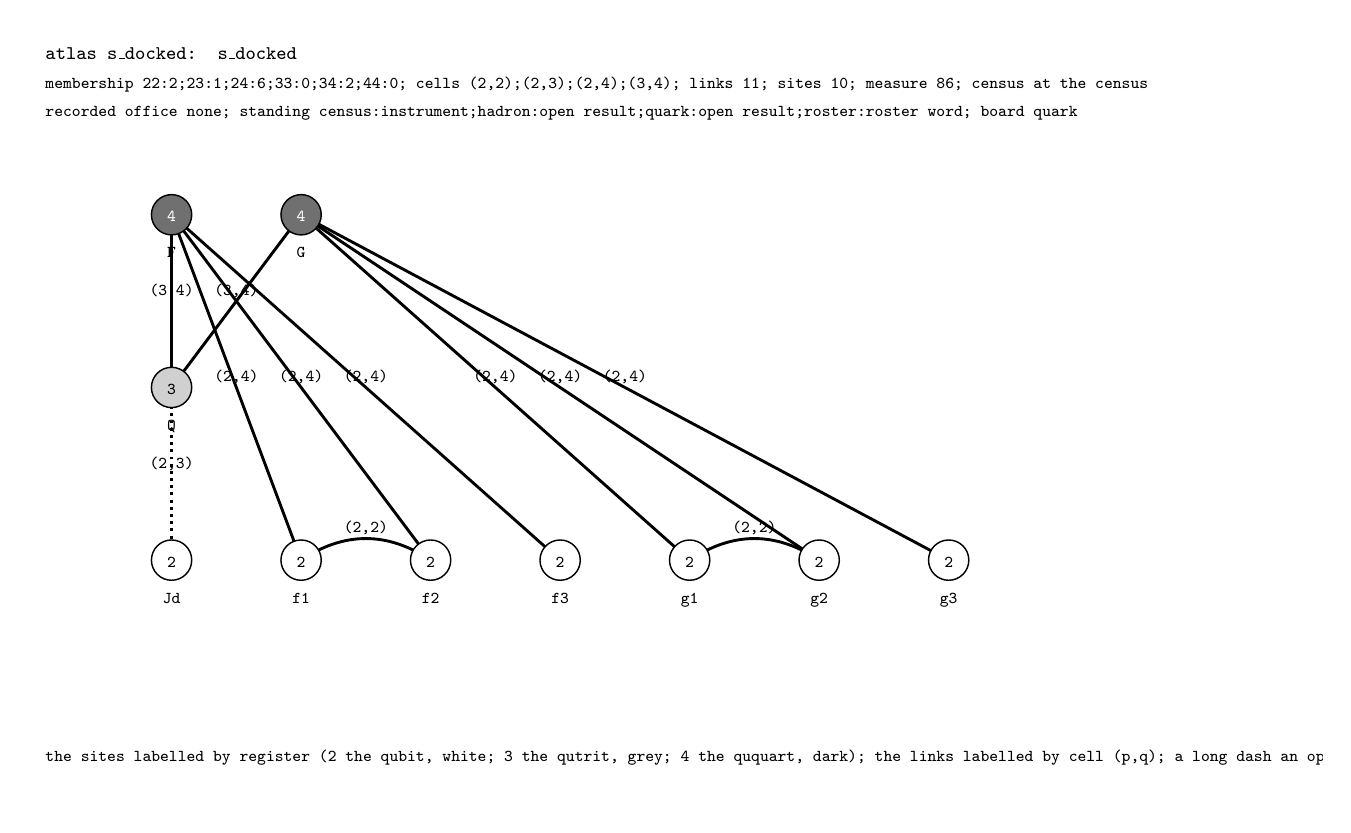
\begin{tikzpicture}[x=0.52pt,y=-0.52pt,baseline]
\clip (0,0) rectangle (900,540);
\fill[white] (0,0) rectangle (900,540);
\node[anchor=base west,inner sep=0pt,text=black,font=\fontsize{6.76}{8.112}\selectfont\ttfamily] at (12,22) {atlas s\_docked: s\_docked};
\node[anchor=base west,inner sep=0pt,text=black,font=\fontsize{6.24}{7.488}\selectfont\ttfamily] at (12,42) {membership 22:2;23:1;24:6;33:0;34:2;44:0; cells (2,2);(2,3);(2,4);(3,4); links 11; sites 10; measure 86; census at the census};
\node[anchor=base west,inner sep=0pt,text=black,font=\fontsize{5.72}{6.864}\selectfont\ttfamily] at (12,62) {recorded office none; standing census:instrument;hadron:open result;quark:open result;roster:roster word; board quark};
\draw[draw=black,line width=1.04pt] (100,130) -- (100,250);
\node[anchor=base,inner sep=0pt,text=black,font=\fontsize{5.72}{6.864}\selectfont\ttfamily] at (100,186) {(3,4)};
\draw[draw=black,line width=1.04pt] (100,130) -- (190,370);
\node[anchor=base,inner sep=0pt,text=black,font=\fontsize{5.72}{6.864}\selectfont\ttfamily] at (145,246) {(2,4)};
\draw[draw=black,line width=1.04pt] (100,130) -- (280,370);
\node[anchor=base,inner sep=0pt,text=black,font=\fontsize{5.72}{6.864}\selectfont\ttfamily] at (190,246) {(2,4)};
\draw[draw=black,line width=1.04pt] (100,130) -- (370,370);
\node[anchor=base,inner sep=0pt,text=black,font=\fontsize{5.72}{6.864}\selectfont\ttfamily] at (235,246) {(2,4)};
\draw[draw=black,line width=1.04pt] (190,130) -- (100,250);
\node[anchor=base,inner sep=0pt,text=black,font=\fontsize{5.72}{6.864}\selectfont\ttfamily] at (145,186) {(3,4)};
\draw[draw=black,line width=1.04pt] (190,130) -- (460,370);
\node[anchor=base,inner sep=0pt,text=black,font=\fontsize{5.72}{6.864}\selectfont\ttfamily] at (325,246) {(2,4)};
\draw[draw=black,line width=1.04pt] (190,130) -- (550,370);
\node[anchor=base,inner sep=0pt,text=black,font=\fontsize{5.72}{6.864}\selectfont\ttfamily] at (370,246) {(2,4)};
\draw[draw=black,line width=1.04pt] (190,130) -- (640,370);
\node[anchor=base,inner sep=0pt,text=black,font=\fontsize{5.72}{6.864}\selectfont\ttfamily] at (415,246) {(2,4)};
\draw[draw=black,line width=1.04pt,dash pattern=on 1.04pt off 1.56pt] (100,370) -- (100,250);
\node[anchor=base,inner sep=0pt,text=black,font=\fontsize{5.72}{6.864}\selectfont\ttfamily] at (100,306) {(2,3)};
\draw[draw=black,line width=1.04pt] (190,370) .. controls (220,350) and (250,350) .. (280,370);
\node[anchor=base,inner sep=0pt,text=black,font=\fontsize{5.72}{6.864}\selectfont\ttfamily] at (235,351) {(2,2)};
\draw[draw=black,line width=1.04pt] (460,370) .. controls (490,350) and (520,350) .. (550,370);
\node[anchor=base,inner sep=0pt,text=black,font=\fontsize{5.72}{6.864}\selectfont\ttfamily] at (505,351) {(2,2)};
\filldraw[fill={rgb,255:red,112;green,112;blue,112},draw=black,line width=0.52pt] (100,130) circle (14);
\node[anchor=base,inner sep=0pt,text=white,font=\fontsize{6.24}{7.488}\selectfont\ttfamily] at (100,135) {4};
\node[anchor=base,inner sep=0pt,text=black,font=\fontsize{5.72}{6.864}\selectfont\ttfamily] at (100,160) {F};
\filldraw[fill={rgb,255:red,112;green,112;blue,112},draw=black,line width=0.52pt] (190,130) circle (14);
\node[anchor=base,inner sep=0pt,text=white,font=\fontsize{6.24}{7.488}\selectfont\ttfamily] at (190,135) {4};
\node[anchor=base,inner sep=0pt,text=black,font=\fontsize{5.72}{6.864}\selectfont\ttfamily] at (190,160) {G};
\filldraw[fill=white,draw=black,line width=0.52pt] (100,370) circle (14);
\node[anchor=base,inner sep=0pt,text=black,font=\fontsize{6.24}{7.488}\selectfont\ttfamily] at (100,375) {2};
\node[anchor=base,inner sep=0pt,text=black,font=\fontsize{5.72}{6.864}\selectfont\ttfamily] at (100,400) {Jd};
\filldraw[fill={rgb,255:red,208;green,208;blue,208},draw=black,line width=0.52pt] (100,250) circle (14);
\node[anchor=base,inner sep=0pt,text=black,font=\fontsize{6.24}{7.488}\selectfont\ttfamily] at (100,255) {3};
\node[anchor=base,inner sep=0pt,text=black,font=\fontsize{5.72}{6.864}\selectfont\ttfamily] at (100,280) {Q};
\filldraw[fill=white,draw=black,line width=0.52pt] (190,370) circle (14);
\node[anchor=base,inner sep=0pt,text=black,font=\fontsize{6.24}{7.488}\selectfont\ttfamily] at (190,375) {2};
\node[anchor=base,inner sep=0pt,text=black,font=\fontsize{5.72}{6.864}\selectfont\ttfamily] at (190,400) {f1};
\filldraw[fill=white,draw=black,line width=0.52pt] (280,370) circle (14);
\node[anchor=base,inner sep=0pt,text=black,font=\fontsize{6.24}{7.488}\selectfont\ttfamily] at (280,375) {2};
\node[anchor=base,inner sep=0pt,text=black,font=\fontsize{5.72}{6.864}\selectfont\ttfamily] at (280,400) {f2};
\filldraw[fill=white,draw=black,line width=0.52pt] (370,370) circle (14);
\node[anchor=base,inner sep=0pt,text=black,font=\fontsize{6.24}{7.488}\selectfont\ttfamily] at (370,375) {2};
\node[anchor=base,inner sep=0pt,text=black,font=\fontsize{5.72}{6.864}\selectfont\ttfamily] at (370,400) {f3};
\filldraw[fill=white,draw=black,line width=0.52pt] (460,370) circle (14);
\node[anchor=base,inner sep=0pt,text=black,font=\fontsize{6.24}{7.488}\selectfont\ttfamily] at (460,375) {2};
\node[anchor=base,inner sep=0pt,text=black,font=\fontsize{5.72}{6.864}\selectfont\ttfamily] at (460,400) {g1};
\filldraw[fill=white,draw=black,line width=0.52pt] (550,370) circle (14);
\node[anchor=base,inner sep=0pt,text=black,font=\fontsize{6.24}{7.488}\selectfont\ttfamily] at (550,375) {2};
\node[anchor=base,inner sep=0pt,text=black,font=\fontsize{5.72}{6.864}\selectfont\ttfamily] at (550,400) {g2};
\filldraw[fill=white,draw=black,line width=0.52pt] (640,370) circle (14);
\node[anchor=base,inner sep=0pt,text=black,font=\fontsize{6.24}{7.488}\selectfont\ttfamily] at (640,375) {2};
\node[anchor=base,inner sep=0pt,text=black,font=\fontsize{5.72}{6.864}\selectfont\ttfamily] at (640,400) {g3};
\node[anchor=base west,inner sep=0pt,text=black,font=\fontsize{5.72}{6.864}\selectfont\ttfamily] at (12,510) {the sites labelled by register (2 the qubit, white; 3 the qutrit, grey; 4 the ququart, dark); the links labelled by cell (p,q); a long dash an open dark link of the neutron row; a short dash a docked link at the rule R1};
\end{tikzpicture}\end{adjustbox}
\caption{\texttt{s\_docked} (the quark), hadron row body: 10 sites, 11 links, the measure 86; the links at the cells (2,2), (2,3), (2,4), (3,4); the membership 22:2; 23:1; 24:6; 33:0; 34:2; 44:0; 1 docked links at the rule R1 (Q-Jd); at the census of the six cells. Drawn at the anatomy atlas as its web, the sites labeled by register and the links by cell, from the hadron spectroscopy at the cap sinks.}\label{fig:VII-6-D540002-s-docked-8fff1f}
\begin{center}\footnotesize\begin{adjustbox}{max width=\linewidth}\begin{tabular}{p{0.26\textwidth}p{0.68\textwidth}}\toprule
recorded office (the slot-count row) & no read of this body at the slot-count row \\
mass register (the mass-register row) & the read KS: the class touching the ququart; the first power 720; the office \texttt{95552332143529/184320000\textbar{}661/225\textbar{}5069/2304000\textbar{}0}; nonzero; met yes; hubs F; G; in-legs q-f; q-g; dressing 9; ports F-f3; G-g3; Q-Jd \\
\bottomrule\end{tabular}\end{adjustbox}\end{center}
\end{figure}
\begin{figure}[H]\centering
\begin{adjustbox}{max width=\linewidth}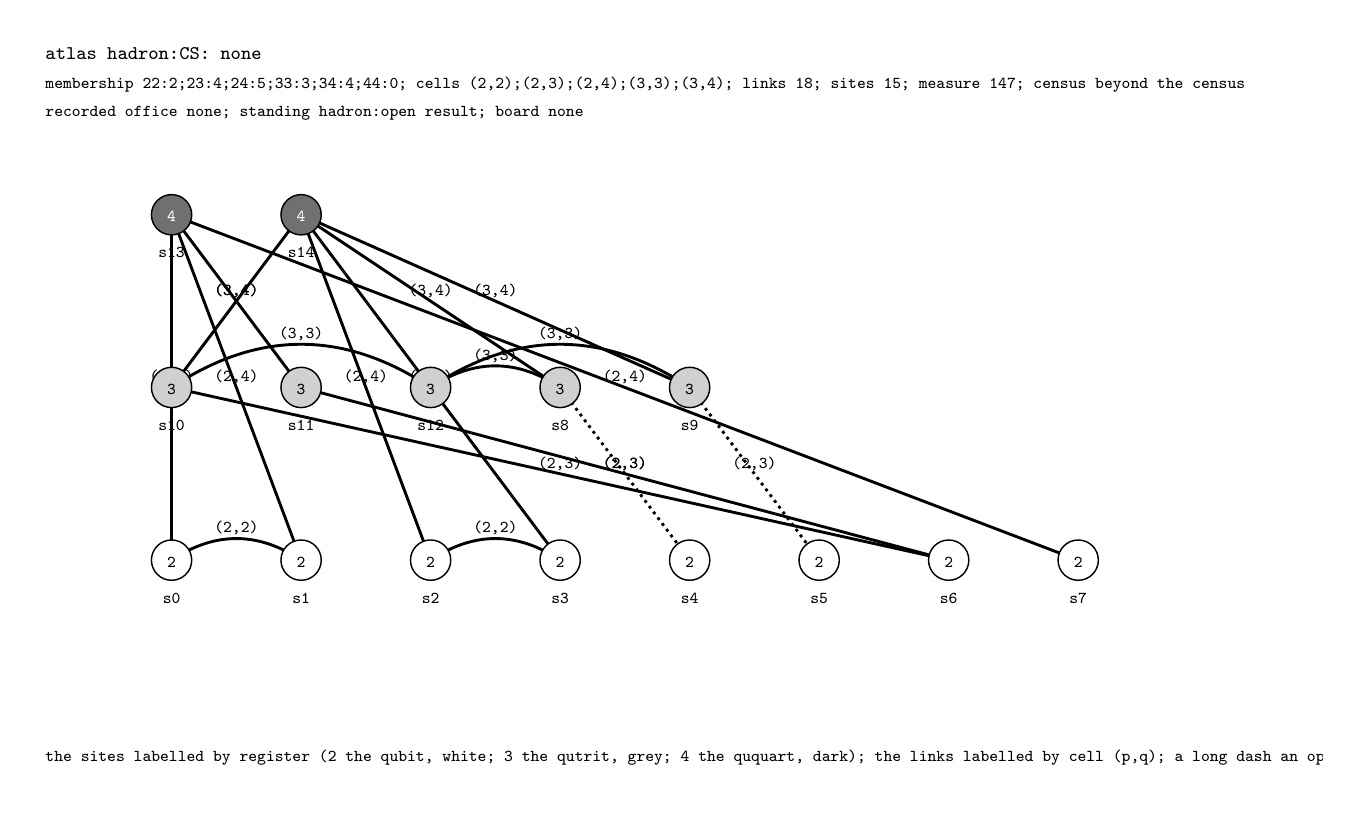
\begin{tikzpicture}[x=0.52pt,y=-0.52pt,baseline]
\clip (0,0) rectangle (900,540);
\fill[white] (0,0) rectangle (900,540);
\node[anchor=base west,inner sep=0pt,text=black,font=\fontsize{6.76}{8.112}\selectfont\ttfamily] at (12,22) {atlas hadron:CS: none};
\node[anchor=base west,inner sep=0pt,text=black,font=\fontsize{6.24}{7.488}\selectfont\ttfamily] at (12,42) {membership 22:2;23:4;24:5;33:3;34:4;44:0; cells (2,2);(2,3);(2,4);(3,3);(3,4); links 18; sites 15; measure 147; census beyond the census};
\node[anchor=base west,inner sep=0pt,text=black,font=\fontsize{5.72}{6.864}\selectfont\ttfamily] at (12,62) {recorded office none; standing hadron:open result; board none};
\draw[draw=black,line width=1.04pt] (100,370) -- (100,130);
\node[anchor=base,inner sep=0pt,text=black,font=\fontsize{5.72}{6.864}\selectfont\ttfamily] at (100,246) {(2,4)};
\draw[draw=black,line width=1.04pt] (100,370) .. controls (130,350) and (160,350) .. (190,370);
\node[anchor=base,inner sep=0pt,text=black,font=\fontsize{5.72}{6.864}\selectfont\ttfamily] at (145,351) {(2,2)};
\draw[draw=black,line width=1.04pt] (190,370) -- (100,130);
\node[anchor=base,inner sep=0pt,text=black,font=\fontsize{5.72}{6.864}\selectfont\ttfamily] at (145,246) {(2,4)};
\draw[draw=black,line width=1.04pt] (100,250) .. controls (160,210) and (220,210) .. (280,250);
\node[anchor=base,inner sep=0pt,text=black,font=\fontsize{5.72}{6.864}\selectfont\ttfamily] at (190,216) {(3,3)};
\draw[draw=black,line width=1.04pt] (100,250) -- (190,130);
\node[anchor=base,inner sep=0pt,text=black,font=\fontsize{5.72}{6.864}\selectfont\ttfamily] at (145,186) {(3,4)};
\draw[draw=black,line width=1.04pt] (100,250) -- (640,370);
\node[anchor=base,inner sep=0pt,text=black,font=\fontsize{5.72}{6.864}\selectfont\ttfamily] at (370,306) {(2,3)};
\draw[draw=black,line width=1.04pt] (190,250) -- (100,130);
\node[anchor=base,inner sep=0pt,text=black,font=\fontsize{5.72}{6.864}\selectfont\ttfamily] at (145,186) {(3,4)};
\draw[draw=black,line width=1.04pt] (190,250) -- (640,370);
\node[anchor=base,inner sep=0pt,text=black,font=\fontsize{5.72}{6.864}\selectfont\ttfamily] at (415,306) {(2,3)};
\draw[draw=black,line width=1.04pt] (280,250) .. controls (310,230) and (340,230) .. (370,250);
\node[anchor=base,inner sep=0pt,text=black,font=\fontsize{5.72}{6.864}\selectfont\ttfamily] at (325,231) {(3,3)};
\draw[draw=black,line width=1.04pt] (280,250) .. controls (340,210) and (400,210) .. (460,250);
\node[anchor=base,inner sep=0pt,text=black,font=\fontsize{5.72}{6.864}\selectfont\ttfamily] at (370,216) {(3,3)};
\draw[draw=black,line width=1.04pt] (100,130) -- (730,370);
\node[anchor=base,inner sep=0pt,text=black,font=\fontsize{5.72}{6.864}\selectfont\ttfamily] at (415,246) {(2,4)};
\draw[draw=black,line width=1.04pt] (190,130) -- (280,370);
\node[anchor=base,inner sep=0pt,text=black,font=\fontsize{5.72}{6.864}\selectfont\ttfamily] at (235,246) {(2,4)};
\draw[draw=black,line width=1.04pt] (190,130) -- (370,370);
\node[anchor=base,inner sep=0pt,text=black,font=\fontsize{5.72}{6.864}\selectfont\ttfamily] at (280,246) {(2,4)};
\draw[draw=black,line width=1.04pt] (190,130) -- (370,250);
\node[anchor=base,inner sep=0pt,text=black,font=\fontsize{5.72}{6.864}\selectfont\ttfamily] at (280,186) {(3,4)};
\draw[draw=black,line width=1.04pt] (190,130) -- (460,250);
\node[anchor=base,inner sep=0pt,text=black,font=\fontsize{5.72}{6.864}\selectfont\ttfamily] at (325,186) {(3,4)};
\draw[draw=black,line width=1.04pt] (280,370) .. controls (310,350) and (340,350) .. (370,370);
\node[anchor=base,inner sep=0pt,text=black,font=\fontsize{5.72}{6.864}\selectfont\ttfamily] at (325,351) {(2,2)};
\draw[draw=black,line width=1.04pt,dash pattern=on 1.04pt off 1.56pt] (460,370) -- (370,250);
\node[anchor=base,inner sep=0pt,text=black,font=\fontsize{5.72}{6.864}\selectfont\ttfamily] at (415,306) {(2,3)};
\draw[draw=black,line width=1.04pt,dash pattern=on 1.04pt off 1.56pt] (550,370) -- (460,250);
\node[anchor=base,inner sep=0pt,text=black,font=\fontsize{5.72}{6.864}\selectfont\ttfamily] at (505,306) {(2,3)};
\filldraw[fill=white,draw=black,line width=0.52pt] (100,370) circle (14);
\node[anchor=base,inner sep=0pt,text=black,font=\fontsize{6.24}{7.488}\selectfont\ttfamily] at (100,375) {2};
\node[anchor=base,inner sep=0pt,text=black,font=\fontsize{5.72}{6.864}\selectfont\ttfamily] at (100,400) {s0};
\filldraw[fill=white,draw=black,line width=0.52pt] (190,370) circle (14);
\node[anchor=base,inner sep=0pt,text=black,font=\fontsize{6.24}{7.488}\selectfont\ttfamily] at (190,375) {2};
\node[anchor=base,inner sep=0pt,text=black,font=\fontsize{5.72}{6.864}\selectfont\ttfamily] at (190,400) {s1};
\filldraw[fill={rgb,255:red,208;green,208;blue,208},draw=black,line width=0.52pt] (100,250) circle (14);
\node[anchor=base,inner sep=0pt,text=black,font=\fontsize{6.24}{7.488}\selectfont\ttfamily] at (100,255) {3};
\node[anchor=base,inner sep=0pt,text=black,font=\fontsize{5.72}{6.864}\selectfont\ttfamily] at (100,280) {s10};
\filldraw[fill={rgb,255:red,208;green,208;blue,208},draw=black,line width=0.52pt] (190,250) circle (14);
\node[anchor=base,inner sep=0pt,text=black,font=\fontsize{6.24}{7.488}\selectfont\ttfamily] at (190,255) {3};
\node[anchor=base,inner sep=0pt,text=black,font=\fontsize{5.72}{6.864}\selectfont\ttfamily] at (190,280) {s11};
\filldraw[fill={rgb,255:red,208;green,208;blue,208},draw=black,line width=0.52pt] (280,250) circle (14);
\node[anchor=base,inner sep=0pt,text=black,font=\fontsize{6.24}{7.488}\selectfont\ttfamily] at (280,255) {3};
\node[anchor=base,inner sep=0pt,text=black,font=\fontsize{5.72}{6.864}\selectfont\ttfamily] at (280,280) {s12};
\filldraw[fill={rgb,255:red,112;green,112;blue,112},draw=black,line width=0.52pt] (100,130) circle (14);
\node[anchor=base,inner sep=0pt,text=white,font=\fontsize{6.24}{7.488}\selectfont\ttfamily] at (100,135) {4};
\node[anchor=base,inner sep=0pt,text=black,font=\fontsize{5.72}{6.864}\selectfont\ttfamily] at (100,160) {s13};
\filldraw[fill={rgb,255:red,112;green,112;blue,112},draw=black,line width=0.52pt] (190,130) circle (14);
\node[anchor=base,inner sep=0pt,text=white,font=\fontsize{6.24}{7.488}\selectfont\ttfamily] at (190,135) {4};
\node[anchor=base,inner sep=0pt,text=black,font=\fontsize{5.72}{6.864}\selectfont\ttfamily] at (190,160) {s14};
\filldraw[fill=white,draw=black,line width=0.52pt] (280,370) circle (14);
\node[anchor=base,inner sep=0pt,text=black,font=\fontsize{6.24}{7.488}\selectfont\ttfamily] at (280,375) {2};
\node[anchor=base,inner sep=0pt,text=black,font=\fontsize{5.72}{6.864}\selectfont\ttfamily] at (280,400) {s2};
\filldraw[fill=white,draw=black,line width=0.52pt] (370,370) circle (14);
\node[anchor=base,inner sep=0pt,text=black,font=\fontsize{6.24}{7.488}\selectfont\ttfamily] at (370,375) {2};
\node[anchor=base,inner sep=0pt,text=black,font=\fontsize{5.72}{6.864}\selectfont\ttfamily] at (370,400) {s3};
\filldraw[fill=white,draw=black,line width=0.52pt] (460,370) circle (14);
\node[anchor=base,inner sep=0pt,text=black,font=\fontsize{6.24}{7.488}\selectfont\ttfamily] at (460,375) {2};
\node[anchor=base,inner sep=0pt,text=black,font=\fontsize{5.72}{6.864}\selectfont\ttfamily] at (460,400) {s4};
\filldraw[fill=white,draw=black,line width=0.52pt] (550,370) circle (14);
\node[anchor=base,inner sep=0pt,text=black,font=\fontsize{6.24}{7.488}\selectfont\ttfamily] at (550,375) {2};
\node[anchor=base,inner sep=0pt,text=black,font=\fontsize{5.72}{6.864}\selectfont\ttfamily] at (550,400) {s5};
\filldraw[fill=white,draw=black,line width=0.52pt] (640,370) circle (14);
\node[anchor=base,inner sep=0pt,text=black,font=\fontsize{6.24}{7.488}\selectfont\ttfamily] at (640,375) {2};
\node[anchor=base,inner sep=0pt,text=black,font=\fontsize{5.72}{6.864}\selectfont\ttfamily] at (640,400) {s6};
\filldraw[fill=white,draw=black,line width=0.52pt] (730,370) circle (14);
\node[anchor=base,inner sep=0pt,text=black,font=\fontsize{6.24}{7.488}\selectfont\ttfamily] at (730,375) {2};
\node[anchor=base,inner sep=0pt,text=black,font=\fontsize{5.72}{6.864}\selectfont\ttfamily] at (730,400) {s7};
\filldraw[fill={rgb,255:red,208;green,208;blue,208},draw=black,line width=0.52pt] (370,250) circle (14);
\node[anchor=base,inner sep=0pt,text=black,font=\fontsize{6.24}{7.488}\selectfont\ttfamily] at (370,255) {3};
\node[anchor=base,inner sep=0pt,text=black,font=\fontsize{5.72}{6.864}\selectfont\ttfamily] at (370,280) {s8};
\filldraw[fill={rgb,255:red,208;green,208;blue,208},draw=black,line width=0.52pt] (460,250) circle (14);
\node[anchor=base,inner sep=0pt,text=black,font=\fontsize{6.24}{7.488}\selectfont\ttfamily] at (460,255) {3};
\node[anchor=base,inner sep=0pt,text=black,font=\fontsize{5.72}{6.864}\selectfont\ttfamily] at (460,280) {s9};
\node[anchor=base west,inner sep=0pt,text=black,font=\fontsize{5.72}{6.864}\selectfont\ttfamily] at (12,510) {the sites labelled by register (2 the qubit, white; 3 the qutrit, grey; 4 the ququart, dark); the links labelled by cell (p,q); a long dash an open dark link of the neutron row; a short dash a docked link at the rule R1};
\end{tikzpicture}\end{adjustbox}
\caption{\texttt{CS of the hadron row}, hadron row body: 15 sites, 18 links, the measure 147; the links at the cells (2,2), (2,3), (2,4), (3,3), (3,4); the membership 22:2; 23:4; 24:5; 33:3; 34:4; 44:0; 2 docked links at the rule R1 (s4-s8; s5-s9); beyond the census of the six cells. Drawn at the anatomy atlas as its web, the sites labeled by register and the links by cell, from the hadron spectroscopy at the cap sinks.}\label{fig:VII-6-D540002-cs-078b31}
\begin{center}\footnotesize\begin{adjustbox}{max width=\linewidth}\begin{tabular}{p{0.26\textwidth}p{0.68\textwidth}}\toprule
recorded office (the slot-count row) & no read of this body at the slot-count row \\
mass register (the mass-register row) & no read of this body at the mass-register row \\
\bottomrule\end{tabular}\end{adjustbox}\end{center}
\end{figure}
\begin{figure}[H]\centering
\begin{adjustbox}{max width=\linewidth}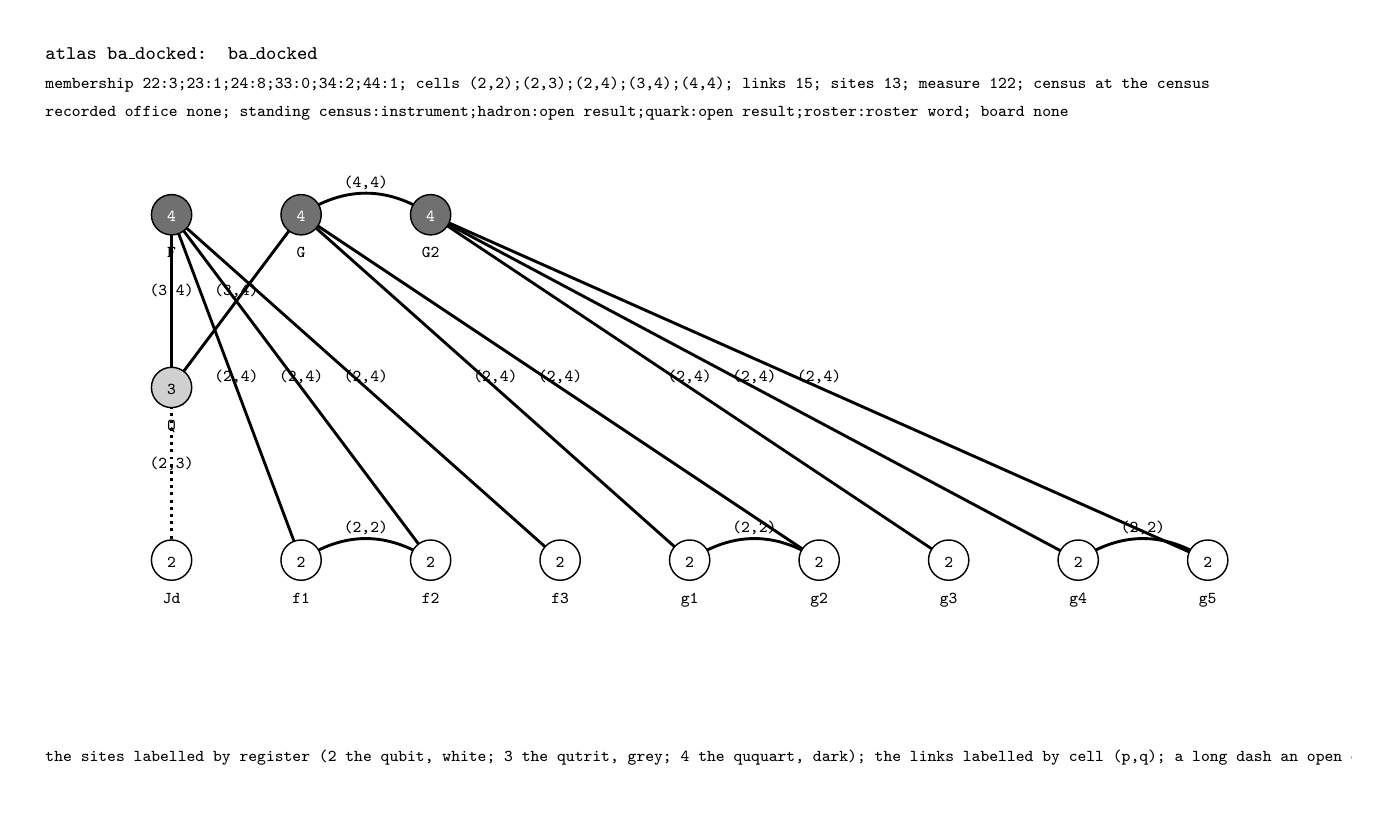
\begin{tikzpicture}[x=0.52pt,y=-0.52pt,baseline]
\clip (0,0) rectangle (920,540);
\fill[white] (0,0) rectangle (920,540);
\node[anchor=base west,inner sep=0pt,text=black,font=\fontsize{6.76}{8.112}\selectfont\ttfamily] at (12,22) {atlas ba\_docked: ba\_docked};
\node[anchor=base west,inner sep=0pt,text=black,font=\fontsize{6.24}{7.488}\selectfont\ttfamily] at (12,42) {membership 22:3;23:1;24:8;33:0;34:2;44:1; cells (2,2);(2,3);(2,4);(3,4);(4,4); links 15; sites 13; measure 122; census at the census};
\node[anchor=base west,inner sep=0pt,text=black,font=\fontsize{5.72}{6.864}\selectfont\ttfamily] at (12,62) {recorded office none; standing census:instrument;hadron:open result;quark:open result;roster:roster word; board none};
\draw[draw=black,line width=1.04pt] (100,130) -- (100,250);
\node[anchor=base,inner sep=0pt,text=black,font=\fontsize{5.72}{6.864}\selectfont\ttfamily] at (100,186) {(3,4)};
\draw[draw=black,line width=1.04pt] (100,130) -- (190,370);
\node[anchor=base,inner sep=0pt,text=black,font=\fontsize{5.72}{6.864}\selectfont\ttfamily] at (145,246) {(2,4)};
\draw[draw=black,line width=1.04pt] (100,130) -- (280,370);
\node[anchor=base,inner sep=0pt,text=black,font=\fontsize{5.72}{6.864}\selectfont\ttfamily] at (190,246) {(2,4)};
\draw[draw=black,line width=1.04pt] (100,130) -- (370,370);
\node[anchor=base,inner sep=0pt,text=black,font=\fontsize{5.72}{6.864}\selectfont\ttfamily] at (235,246) {(2,4)};
\draw[draw=black,line width=1.04pt] (190,130) .. controls (220,110) and (250,110) .. (280,130);
\node[anchor=base,inner sep=0pt,text=black,font=\fontsize{5.72}{6.864}\selectfont\ttfamily] at (235,111) {(4,4)};
\draw[draw=black,line width=1.04pt] (190,130) -- (100,250);
\node[anchor=base,inner sep=0pt,text=black,font=\fontsize{5.72}{6.864}\selectfont\ttfamily] at (145,186) {(3,4)};
\draw[draw=black,line width=1.04pt] (190,130) -- (460,370);
\node[anchor=base,inner sep=0pt,text=black,font=\fontsize{5.72}{6.864}\selectfont\ttfamily] at (325,246) {(2,4)};
\draw[draw=black,line width=1.04pt] (190,130) -- (550,370);
\node[anchor=base,inner sep=0pt,text=black,font=\fontsize{5.72}{6.864}\selectfont\ttfamily] at (370,246) {(2,4)};
\draw[draw=black,line width=1.04pt] (280,130) -- (640,370);
\node[anchor=base,inner sep=0pt,text=black,font=\fontsize{5.72}{6.864}\selectfont\ttfamily] at (460,246) {(2,4)};
\draw[draw=black,line width=1.04pt] (280,130) -- (730,370);
\node[anchor=base,inner sep=0pt,text=black,font=\fontsize{5.72}{6.864}\selectfont\ttfamily] at (505,246) {(2,4)};
\draw[draw=black,line width=1.04pt] (280,130) -- (820,370);
\node[anchor=base,inner sep=0pt,text=black,font=\fontsize{5.72}{6.864}\selectfont\ttfamily] at (550,246) {(2,4)};
\draw[draw=black,line width=1.04pt,dash pattern=on 1.04pt off 1.56pt] (100,370) -- (100,250);
\node[anchor=base,inner sep=0pt,text=black,font=\fontsize{5.72}{6.864}\selectfont\ttfamily] at (100,306) {(2,3)};
\draw[draw=black,line width=1.04pt] (190,370) .. controls (220,350) and (250,350) .. (280,370);
\node[anchor=base,inner sep=0pt,text=black,font=\fontsize{5.72}{6.864}\selectfont\ttfamily] at (235,351) {(2,2)};
\draw[draw=black,line width=1.04pt] (460,370) .. controls (490,350) and (520,350) .. (550,370);
\node[anchor=base,inner sep=0pt,text=black,font=\fontsize{5.72}{6.864}\selectfont\ttfamily] at (505,351) {(2,2)};
\draw[draw=black,line width=1.04pt] (730,370) .. controls (760,350) and (790,350) .. (820,370);
\node[anchor=base,inner sep=0pt,text=black,font=\fontsize{5.72}{6.864}\selectfont\ttfamily] at (775,351) {(2,2)};
\filldraw[fill={rgb,255:red,112;green,112;blue,112},draw=black,line width=0.52pt] (100,130) circle (14);
\node[anchor=base,inner sep=0pt,text=white,font=\fontsize{6.24}{7.488}\selectfont\ttfamily] at (100,135) {4};
\node[anchor=base,inner sep=0pt,text=black,font=\fontsize{5.72}{6.864}\selectfont\ttfamily] at (100,160) {F};
\filldraw[fill={rgb,255:red,112;green,112;blue,112},draw=black,line width=0.52pt] (190,130) circle (14);
\node[anchor=base,inner sep=0pt,text=white,font=\fontsize{6.24}{7.488}\selectfont\ttfamily] at (190,135) {4};
\node[anchor=base,inner sep=0pt,text=black,font=\fontsize{5.72}{6.864}\selectfont\ttfamily] at (190,160) {G};
\filldraw[fill={rgb,255:red,112;green,112;blue,112},draw=black,line width=0.52pt] (280,130) circle (14);
\node[anchor=base,inner sep=0pt,text=white,font=\fontsize{6.24}{7.488}\selectfont\ttfamily] at (280,135) {4};
\node[anchor=base,inner sep=0pt,text=black,font=\fontsize{5.72}{6.864}\selectfont\ttfamily] at (280,160) {G2};
\filldraw[fill=white,draw=black,line width=0.52pt] (100,370) circle (14);
\node[anchor=base,inner sep=0pt,text=black,font=\fontsize{6.24}{7.488}\selectfont\ttfamily] at (100,375) {2};
\node[anchor=base,inner sep=0pt,text=black,font=\fontsize{5.72}{6.864}\selectfont\ttfamily] at (100,400) {Jd};
\filldraw[fill={rgb,255:red,208;green,208;blue,208},draw=black,line width=0.52pt] (100,250) circle (14);
\node[anchor=base,inner sep=0pt,text=black,font=\fontsize{6.24}{7.488}\selectfont\ttfamily] at (100,255) {3};
\node[anchor=base,inner sep=0pt,text=black,font=\fontsize{5.72}{6.864}\selectfont\ttfamily] at (100,280) {Q};
\filldraw[fill=white,draw=black,line width=0.52pt] (190,370) circle (14);
\node[anchor=base,inner sep=0pt,text=black,font=\fontsize{6.24}{7.488}\selectfont\ttfamily] at (190,375) {2};
\node[anchor=base,inner sep=0pt,text=black,font=\fontsize{5.72}{6.864}\selectfont\ttfamily] at (190,400) {f1};
\filldraw[fill=white,draw=black,line width=0.52pt] (280,370) circle (14);
\node[anchor=base,inner sep=0pt,text=black,font=\fontsize{6.24}{7.488}\selectfont\ttfamily] at (280,375) {2};
\node[anchor=base,inner sep=0pt,text=black,font=\fontsize{5.72}{6.864}\selectfont\ttfamily] at (280,400) {f2};
\filldraw[fill=white,draw=black,line width=0.52pt] (370,370) circle (14);
\node[anchor=base,inner sep=0pt,text=black,font=\fontsize{6.24}{7.488}\selectfont\ttfamily] at (370,375) {2};
\node[anchor=base,inner sep=0pt,text=black,font=\fontsize{5.72}{6.864}\selectfont\ttfamily] at (370,400) {f3};
\filldraw[fill=white,draw=black,line width=0.52pt] (460,370) circle (14);
\node[anchor=base,inner sep=0pt,text=black,font=\fontsize{6.24}{7.488}\selectfont\ttfamily] at (460,375) {2};
\node[anchor=base,inner sep=0pt,text=black,font=\fontsize{5.72}{6.864}\selectfont\ttfamily] at (460,400) {g1};
\filldraw[fill=white,draw=black,line width=0.52pt] (550,370) circle (14);
\node[anchor=base,inner sep=0pt,text=black,font=\fontsize{6.24}{7.488}\selectfont\ttfamily] at (550,375) {2};
\node[anchor=base,inner sep=0pt,text=black,font=\fontsize{5.72}{6.864}\selectfont\ttfamily] at (550,400) {g2};
\filldraw[fill=white,draw=black,line width=0.52pt] (640,370) circle (14);
\node[anchor=base,inner sep=0pt,text=black,font=\fontsize{6.24}{7.488}\selectfont\ttfamily] at (640,375) {2};
\node[anchor=base,inner sep=0pt,text=black,font=\fontsize{5.72}{6.864}\selectfont\ttfamily] at (640,400) {g3};
\filldraw[fill=white,draw=black,line width=0.52pt] (730,370) circle (14);
\node[anchor=base,inner sep=0pt,text=black,font=\fontsize{6.24}{7.488}\selectfont\ttfamily] at (730,375) {2};
\node[anchor=base,inner sep=0pt,text=black,font=\fontsize{5.72}{6.864}\selectfont\ttfamily] at (730,400) {g4};
\filldraw[fill=white,draw=black,line width=0.52pt] (820,370) circle (14);
\node[anchor=base,inner sep=0pt,text=black,font=\fontsize{6.24}{7.488}\selectfont\ttfamily] at (820,375) {2};
\node[anchor=base,inner sep=0pt,text=black,font=\fontsize{5.72}{6.864}\selectfont\ttfamily] at (820,400) {g5};
\node[anchor=base west,inner sep=0pt,text=black,font=\fontsize{5.72}{6.864}\selectfont\ttfamily] at (12,510) {the sites labelled by register (2 the qubit, white; 3 the qutrit, grey; 4 the ququart, dark); the links labelled by cell (p,q); a long dash an open dark link of the neutron row; a short dash a docked link at the rule R1};
\end{tikzpicture}\end{adjustbox}
\caption{\texttt{ba\_docked}, hadron row body: 13 sites, 15 links, the measure 122; the links at the cells (2,2), (2,3), (2,4), (3,4), (4,4); the membership 22:3; 23:1; 24:8; 33:0; 34:2; 44:1; 1 docked links at the rule R1 (Q-Jd); at the census of the six cells. Drawn at the anatomy atlas as its web, the sites labeled by register and the links by cell, from the hadron spectroscopy at the cap sinks.}\label{fig:VII-6-D540002-ba-docked-7309c8}
\begin{center}\footnotesize\begin{adjustbox}{max width=\linewidth}\begin{tabular}{p{0.26\textwidth}p{0.68\textwidth}}\toprule
recorded office (the slot-count row) & no read of this body at the slot-count row \\
mass register (the mass-register row) & the read kba: the class touching the ququart; the first power 1044; the office \texttt{5 022 456 423 459 713/4608000000\textbar{}219/50\textbar{}5069/2304000\textbar{}0}; nonzero; met yes; hubs F; G; G2; in-legs q-f; q-g; dressing 9; ports F-f3; G2-g3; Q-Jd \\
\bottomrule\end{tabular}\end{adjustbox}\end{center}
\end{figure}
\begin{figure}[H]\centering
\begin{adjustbox}{max width=\linewidth}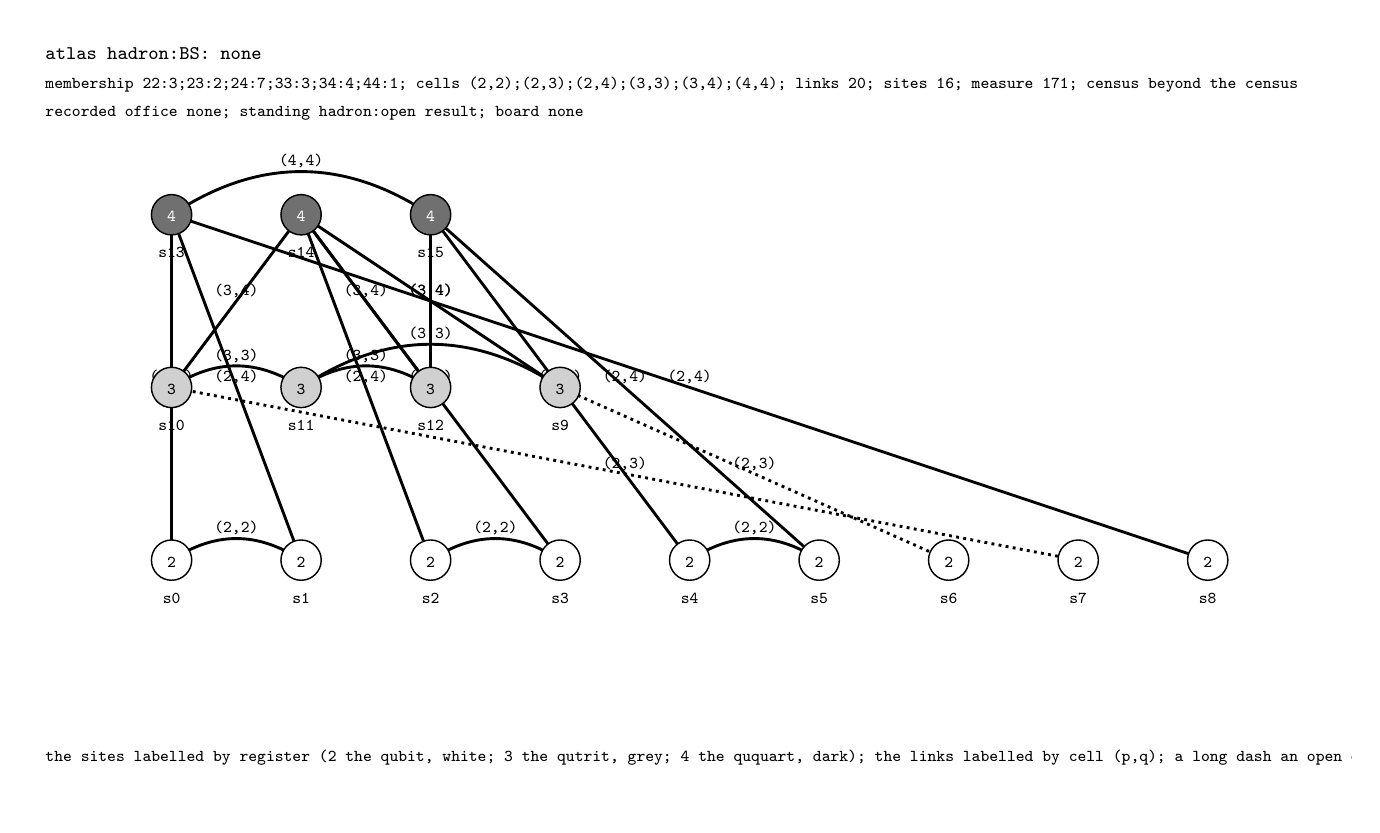
\begin{tikzpicture}[x=0.52pt,y=-0.52pt,baseline]
\clip (0,0) rectangle (920,540);
\fill[white] (0,0) rectangle (920,540);
\node[anchor=base west,inner sep=0pt,text=black,font=\fontsize{6.76}{8.112}\selectfont\ttfamily] at (12,22) {atlas hadron:BS: none};
\node[anchor=base west,inner sep=0pt,text=black,font=\fontsize{6.24}{7.488}\selectfont\ttfamily] at (12,42) {membership 22:3;23:2;24:7;33:3;34:4;44:1; cells (2,2);(2,3);(2,4);(3,3);(3,4);(4,4); links 20; sites 16; measure 171; census beyond the census};
\node[anchor=base west,inner sep=0pt,text=black,font=\fontsize{5.72}{6.864}\selectfont\ttfamily] at (12,62) {recorded office none; standing hadron:open result; board none};
\draw[draw=black,line width=1.04pt] (100,370) -- (100,130);
\node[anchor=base,inner sep=0pt,text=black,font=\fontsize{5.72}{6.864}\selectfont\ttfamily] at (100,246) {(2,4)};
\draw[draw=black,line width=1.04pt] (100,370) .. controls (130,350) and (160,350) .. (190,370);
\node[anchor=base,inner sep=0pt,text=black,font=\fontsize{5.72}{6.864}\selectfont\ttfamily] at (145,351) {(2,2)};
\draw[draw=black,line width=1.04pt] (190,370) -- (100,130);
\node[anchor=base,inner sep=0pt,text=black,font=\fontsize{5.72}{6.864}\selectfont\ttfamily] at (145,246) {(2,4)};
\draw[draw=black,line width=1.04pt] (100,250) .. controls (130,230) and (160,230) .. (190,250);
\node[anchor=base,inner sep=0pt,text=black,font=\fontsize{5.72}{6.864}\selectfont\ttfamily] at (145,231) {(3,3)};
\draw[draw=black,line width=1.04pt] (100,250) -- (190,130);
\node[anchor=base,inner sep=0pt,text=black,font=\fontsize{5.72}{6.864}\selectfont\ttfamily] at (145,186) {(3,4)};
\draw[draw=black,line width=1.04pt,dash pattern=on 1.04pt off 1.56pt] (100,250) -- (730,370);
\node[anchor=base,inner sep=0pt,text=black,font=\fontsize{5.72}{6.864}\selectfont\ttfamily] at (415,306) {(2,3)};
\draw[draw=black,line width=1.04pt] (190,250) .. controls (220,230) and (250,230) .. (280,250);
\node[anchor=base,inner sep=0pt,text=black,font=\fontsize{5.72}{6.864}\selectfont\ttfamily] at (235,231) {(3,3)};
\draw[draw=black,line width=1.04pt] (190,250) .. controls (250,210) and (310,210) .. (370,250);
\node[anchor=base,inner sep=0pt,text=black,font=\fontsize{5.72}{6.864}\selectfont\ttfamily] at (280,216) {(3,3)};
\draw[draw=black,line width=1.04pt] (280,250) -- (190,130);
\node[anchor=base,inner sep=0pt,text=black,font=\fontsize{5.72}{6.864}\selectfont\ttfamily] at (235,186) {(3,4)};
\draw[draw=black,line width=1.04pt] (280,250) -- (280,130);
\node[anchor=base,inner sep=0pt,text=black,font=\fontsize{5.72}{6.864}\selectfont\ttfamily] at (280,186) {(3,4)};
\draw[draw=black,line width=1.04pt] (100,130) .. controls (160,90) and (220,90) .. (280,130);
\node[anchor=base,inner sep=0pt,text=black,font=\fontsize{5.72}{6.864}\selectfont\ttfamily] at (190,96) {(4,4)};
\draw[draw=black,line width=1.04pt] (100,130) -- (820,370);
\node[anchor=base,inner sep=0pt,text=black,font=\fontsize{5.72}{6.864}\selectfont\ttfamily] at (460,246) {(2,4)};
\draw[draw=black,line width=1.04pt] (190,130) -- (280,370);
\node[anchor=base,inner sep=0pt,text=black,font=\fontsize{5.72}{6.864}\selectfont\ttfamily] at (235,246) {(2,4)};
\draw[draw=black,line width=1.04pt] (190,130) -- (370,370);
\node[anchor=base,inner sep=0pt,text=black,font=\fontsize{5.72}{6.864}\selectfont\ttfamily] at (280,246) {(2,4)};
\draw[draw=black,line width=1.04pt] (190,130) -- (370,250);
\node[anchor=base,inner sep=0pt,text=black,font=\fontsize{5.72}{6.864}\selectfont\ttfamily] at (280,186) {(3,4)};
\draw[draw=black,line width=1.04pt] (280,130) -- (460,370);
\node[anchor=base,inner sep=0pt,text=black,font=\fontsize{5.72}{6.864}\selectfont\ttfamily] at (370,246) {(2,4)};
\draw[draw=black,line width=1.04pt] (280,130) -- (550,370);
\node[anchor=base,inner sep=0pt,text=black,font=\fontsize{5.72}{6.864}\selectfont\ttfamily] at (415,246) {(2,4)};
\draw[draw=black,line width=1.04pt] (280,370) .. controls (310,350) and (340,350) .. (370,370);
\node[anchor=base,inner sep=0pt,text=black,font=\fontsize{5.72}{6.864}\selectfont\ttfamily] at (325,351) {(2,2)};
\draw[draw=black,line width=1.04pt] (460,370) .. controls (490,350) and (520,350) .. (550,370);
\node[anchor=base,inner sep=0pt,text=black,font=\fontsize{5.72}{6.864}\selectfont\ttfamily] at (505,351) {(2,2)};
\draw[draw=black,line width=1.04pt,dash pattern=on 1.04pt off 1.56pt] (640,370) -- (370,250);
\node[anchor=base,inner sep=0pt,text=black,font=\fontsize{5.72}{6.864}\selectfont\ttfamily] at (505,306) {(2,3)};
\filldraw[fill=white,draw=black,line width=0.52pt] (100,370) circle (14);
\node[anchor=base,inner sep=0pt,text=black,font=\fontsize{6.24}{7.488}\selectfont\ttfamily] at (100,375) {2};
\node[anchor=base,inner sep=0pt,text=black,font=\fontsize{5.72}{6.864}\selectfont\ttfamily] at (100,400) {s0};
\filldraw[fill=white,draw=black,line width=0.52pt] (190,370) circle (14);
\node[anchor=base,inner sep=0pt,text=black,font=\fontsize{6.24}{7.488}\selectfont\ttfamily] at (190,375) {2};
\node[anchor=base,inner sep=0pt,text=black,font=\fontsize{5.72}{6.864}\selectfont\ttfamily] at (190,400) {s1};
\filldraw[fill={rgb,255:red,208;green,208;blue,208},draw=black,line width=0.52pt] (100,250) circle (14);
\node[anchor=base,inner sep=0pt,text=black,font=\fontsize{6.24}{7.488}\selectfont\ttfamily] at (100,255) {3};
\node[anchor=base,inner sep=0pt,text=black,font=\fontsize{5.72}{6.864}\selectfont\ttfamily] at (100,280) {s10};
\filldraw[fill={rgb,255:red,208;green,208;blue,208},draw=black,line width=0.52pt] (190,250) circle (14);
\node[anchor=base,inner sep=0pt,text=black,font=\fontsize{6.24}{7.488}\selectfont\ttfamily] at (190,255) {3};
\node[anchor=base,inner sep=0pt,text=black,font=\fontsize{5.72}{6.864}\selectfont\ttfamily] at (190,280) {s11};
\filldraw[fill={rgb,255:red,208;green,208;blue,208},draw=black,line width=0.52pt] (280,250) circle (14);
\node[anchor=base,inner sep=0pt,text=black,font=\fontsize{6.24}{7.488}\selectfont\ttfamily] at (280,255) {3};
\node[anchor=base,inner sep=0pt,text=black,font=\fontsize{5.72}{6.864}\selectfont\ttfamily] at (280,280) {s12};
\filldraw[fill={rgb,255:red,112;green,112;blue,112},draw=black,line width=0.52pt] (100,130) circle (14);
\node[anchor=base,inner sep=0pt,text=white,font=\fontsize{6.24}{7.488}\selectfont\ttfamily] at (100,135) {4};
\node[anchor=base,inner sep=0pt,text=black,font=\fontsize{5.72}{6.864}\selectfont\ttfamily] at (100,160) {s13};
\filldraw[fill={rgb,255:red,112;green,112;blue,112},draw=black,line width=0.52pt] (190,130) circle (14);
\node[anchor=base,inner sep=0pt,text=white,font=\fontsize{6.24}{7.488}\selectfont\ttfamily] at (190,135) {4};
\node[anchor=base,inner sep=0pt,text=black,font=\fontsize{5.72}{6.864}\selectfont\ttfamily] at (190,160) {s14};
\filldraw[fill={rgb,255:red,112;green,112;blue,112},draw=black,line width=0.52pt] (280,130) circle (14);
\node[anchor=base,inner sep=0pt,text=white,font=\fontsize{6.24}{7.488}\selectfont\ttfamily] at (280,135) {4};
\node[anchor=base,inner sep=0pt,text=black,font=\fontsize{5.72}{6.864}\selectfont\ttfamily] at (280,160) {s15};
\filldraw[fill=white,draw=black,line width=0.52pt] (280,370) circle (14);
\node[anchor=base,inner sep=0pt,text=black,font=\fontsize{6.24}{7.488}\selectfont\ttfamily] at (280,375) {2};
\node[anchor=base,inner sep=0pt,text=black,font=\fontsize{5.72}{6.864}\selectfont\ttfamily] at (280,400) {s2};
\filldraw[fill=white,draw=black,line width=0.52pt] (370,370) circle (14);
\node[anchor=base,inner sep=0pt,text=black,font=\fontsize{6.24}{7.488}\selectfont\ttfamily] at (370,375) {2};
\node[anchor=base,inner sep=0pt,text=black,font=\fontsize{5.72}{6.864}\selectfont\ttfamily] at (370,400) {s3};
\filldraw[fill=white,draw=black,line width=0.52pt] (460,370) circle (14);
\node[anchor=base,inner sep=0pt,text=black,font=\fontsize{6.24}{7.488}\selectfont\ttfamily] at (460,375) {2};
\node[anchor=base,inner sep=0pt,text=black,font=\fontsize{5.72}{6.864}\selectfont\ttfamily] at (460,400) {s4};
\filldraw[fill=white,draw=black,line width=0.52pt] (550,370) circle (14);
\node[anchor=base,inner sep=0pt,text=black,font=\fontsize{6.24}{7.488}\selectfont\ttfamily] at (550,375) {2};
\node[anchor=base,inner sep=0pt,text=black,font=\fontsize{5.72}{6.864}\selectfont\ttfamily] at (550,400) {s5};
\filldraw[fill=white,draw=black,line width=0.52pt] (640,370) circle (14);
\node[anchor=base,inner sep=0pt,text=black,font=\fontsize{6.24}{7.488}\selectfont\ttfamily] at (640,375) {2};
\node[anchor=base,inner sep=0pt,text=black,font=\fontsize{5.72}{6.864}\selectfont\ttfamily] at (640,400) {s6};
\filldraw[fill=white,draw=black,line width=0.52pt] (730,370) circle (14);
\node[anchor=base,inner sep=0pt,text=black,font=\fontsize{6.24}{7.488}\selectfont\ttfamily] at (730,375) {2};
\node[anchor=base,inner sep=0pt,text=black,font=\fontsize{5.72}{6.864}\selectfont\ttfamily] at (730,400) {s7};
\filldraw[fill=white,draw=black,line width=0.52pt] (820,370) circle (14);
\node[anchor=base,inner sep=0pt,text=black,font=\fontsize{6.24}{7.488}\selectfont\ttfamily] at (820,375) {2};
\node[anchor=base,inner sep=0pt,text=black,font=\fontsize{5.72}{6.864}\selectfont\ttfamily] at (820,400) {s8};
\filldraw[fill={rgb,255:red,208;green,208;blue,208},draw=black,line width=0.52pt] (370,250) circle (14);
\node[anchor=base,inner sep=0pt,text=black,font=\fontsize{6.24}{7.488}\selectfont\ttfamily] at (370,255) {3};
\node[anchor=base,inner sep=0pt,text=black,font=\fontsize{5.72}{6.864}\selectfont\ttfamily] at (370,280) {s9};
\node[anchor=base west,inner sep=0pt,text=black,font=\fontsize{5.72}{6.864}\selectfont\ttfamily] at (12,510) {the sites labelled by register (2 the qubit, white; 3 the qutrit, grey; 4 the ququart, dark); the links labelled by cell (p,q); a long dash an open dark link of the neutron row; a short dash a docked link at the rule R1};
\end{tikzpicture}\end{adjustbox}
\caption{\texttt{BS of the hadron row}, hadron row body: 16 sites, 20 links, the measure 171; the links at the cells (2,2), (2,3), (2,4), (3,3), (3,4), (4,4); the membership 22:3; 23:2; 24:7; 33:3; 34:4; 44:1; 2 docked links at the rule R1 (s6-s9; s7-s10); beyond the census of the six cells. Drawn at the anatomy atlas as its web, the sites labeled by register and the links by cell, from the hadron spectroscopy at the cap sinks.}\label{fig:VII-6-D540002-bs-dfdd5c}
\begin{center}\footnotesize\begin{adjustbox}{max width=\linewidth}\begin{tabular}{p{0.26\textwidth}p{0.68\textwidth}}\toprule
recorded office (the slot-count row) & no read of this body at the slot-count row \\
mass register (the mass-register row) & no read of this body at the mass-register row \\
\bottomrule\end{tabular}\end{adjustbox}\end{center}
\end{figure}
\begin{figure}[H]\centering
\begin{adjustbox}{max width=\linewidth}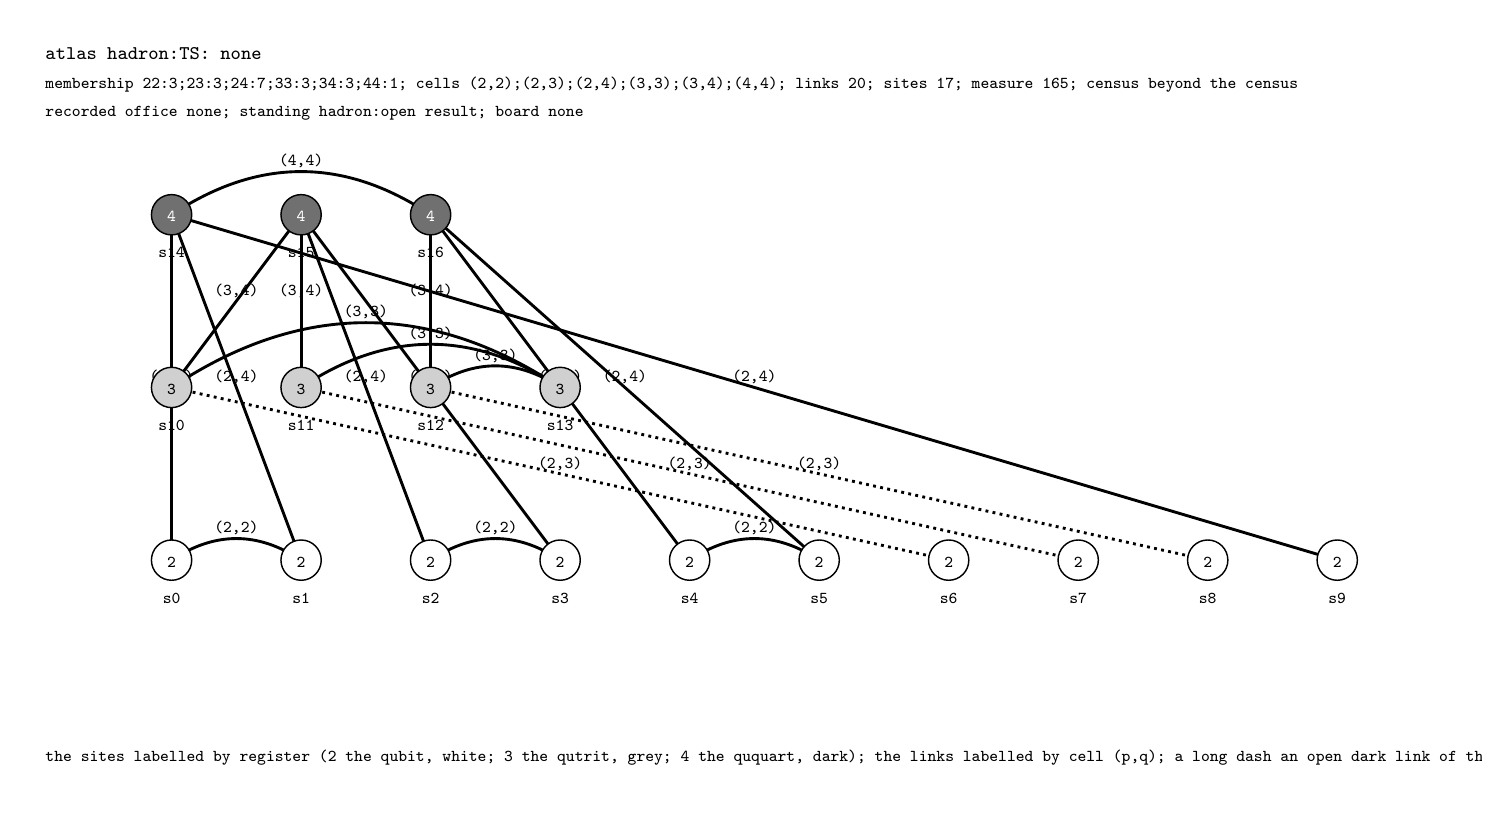
\begin{tikzpicture}[x=0.52pt,y=-0.52pt,baseline]
\clip (0,0) rectangle (1010,540);
\fill[white] (0,0) rectangle (1010,540);
\node[anchor=base west,inner sep=0pt,text=black,font=\fontsize{6.76}{8.112}\selectfont\ttfamily] at (12,22) {atlas hadron:TS: none};
\node[anchor=base west,inner sep=0pt,text=black,font=\fontsize{6.24}{7.488}\selectfont\ttfamily] at (12,42) {membership 22:3;23:3;24:7;33:3;34:3;44:1; cells (2,2);(2,3);(2,4);(3,3);(3,4);(4,4); links 20; sites 17; measure 165; census beyond the census};
\node[anchor=base west,inner sep=0pt,text=black,font=\fontsize{5.72}{6.864}\selectfont\ttfamily] at (12,62) {recorded office none; standing hadron:open result; board none};
\draw[draw=black,line width=1.04pt] (100,370) -- (100,130);
\node[anchor=base,inner sep=0pt,text=black,font=\fontsize{5.72}{6.864}\selectfont\ttfamily] at (100,246) {(2,4)};
\draw[draw=black,line width=1.04pt] (100,370) .. controls (130,350) and (160,350) .. (190,370);
\node[anchor=base,inner sep=0pt,text=black,font=\fontsize{5.72}{6.864}\selectfont\ttfamily] at (145,351) {(2,2)};
\draw[draw=black,line width=1.04pt] (190,370) -- (100,130);
\node[anchor=base,inner sep=0pt,text=black,font=\fontsize{5.72}{6.864}\selectfont\ttfamily] at (145,246) {(2,4)};
\draw[draw=black,line width=1.04pt] (100,250) .. controls (190,190) and (280,190) .. (370,250);
\node[anchor=base,inner sep=0pt,text=black,font=\fontsize{5.72}{6.864}\selectfont\ttfamily] at (235,201) {(3,3)};
\draw[draw=black,line width=1.04pt] (100,250) -- (190,130);
\node[anchor=base,inner sep=0pt,text=black,font=\fontsize{5.72}{6.864}\selectfont\ttfamily] at (145,186) {(3,4)};
\draw[draw=black,line width=1.04pt,dash pattern=on 1.04pt off 1.56pt] (100,250) -- (640,370);
\node[anchor=base,inner sep=0pt,text=black,font=\fontsize{5.72}{6.864}\selectfont\ttfamily] at (370,306) {(2,3)};
\draw[draw=black,line width=1.04pt] (190,250) .. controls (250,210) and (310,210) .. (370,250);
\node[anchor=base,inner sep=0pt,text=black,font=\fontsize{5.72}{6.864}\selectfont\ttfamily] at (280,216) {(3,3)};
\draw[draw=black,line width=1.04pt] (190,250) -- (190,130);
\node[anchor=base,inner sep=0pt,text=black,font=\fontsize{5.72}{6.864}\selectfont\ttfamily] at (190,186) {(3,4)};
\draw[draw=black,line width=1.04pt,dash pattern=on 1.04pt off 1.56pt] (190,250) -- (730,370);
\node[anchor=base,inner sep=0pt,text=black,font=\fontsize{5.72}{6.864}\selectfont\ttfamily] at (460,306) {(2,3)};
\draw[draw=black,line width=1.04pt] (280,250) .. controls (310,230) and (340,230) .. (370,250);
\node[anchor=base,inner sep=0pt,text=black,font=\fontsize{5.72}{6.864}\selectfont\ttfamily] at (325,231) {(3,3)};
\draw[draw=black,line width=1.04pt] (280,250) -- (280,130);
\node[anchor=base,inner sep=0pt,text=black,font=\fontsize{5.72}{6.864}\selectfont\ttfamily] at (280,186) {(3,4)};
\draw[draw=black,line width=1.04pt,dash pattern=on 1.04pt off 1.56pt] (280,250) -- (820,370);
\node[anchor=base,inner sep=0pt,text=black,font=\fontsize{5.72}{6.864}\selectfont\ttfamily] at (550,306) {(2,3)};
\draw[draw=black,line width=1.04pt] (100,130) .. controls (160,90) and (220,90) .. (280,130);
\node[anchor=base,inner sep=0pt,text=black,font=\fontsize{5.72}{6.864}\selectfont\ttfamily] at (190,96) {(4,4)};
\draw[draw=black,line width=1.04pt] (100,130) -- (910,370);
\node[anchor=base,inner sep=0pt,text=black,font=\fontsize{5.72}{6.864}\selectfont\ttfamily] at (505,246) {(2,4)};
\draw[draw=black,line width=1.04pt] (190,130) -- (280,370);
\node[anchor=base,inner sep=0pt,text=black,font=\fontsize{5.72}{6.864}\selectfont\ttfamily] at (235,246) {(2,4)};
\draw[draw=black,line width=1.04pt] (190,130) -- (370,370);
\node[anchor=base,inner sep=0pt,text=black,font=\fontsize{5.72}{6.864}\selectfont\ttfamily] at (280,246) {(2,4)};
\draw[draw=black,line width=1.04pt] (280,130) -- (460,370);
\node[anchor=base,inner sep=0pt,text=black,font=\fontsize{5.72}{6.864}\selectfont\ttfamily] at (370,246) {(2,4)};
\draw[draw=black,line width=1.04pt] (280,130) -- (550,370);
\node[anchor=base,inner sep=0pt,text=black,font=\fontsize{5.72}{6.864}\selectfont\ttfamily] at (415,246) {(2,4)};
\draw[draw=black,line width=1.04pt] (280,370) .. controls (310,350) and (340,350) .. (370,370);
\node[anchor=base,inner sep=0pt,text=black,font=\fontsize{5.72}{6.864}\selectfont\ttfamily] at (325,351) {(2,2)};
\draw[draw=black,line width=1.04pt] (460,370) .. controls (490,350) and (520,350) .. (550,370);
\node[anchor=base,inner sep=0pt,text=black,font=\fontsize{5.72}{6.864}\selectfont\ttfamily] at (505,351) {(2,2)};
\filldraw[fill=white,draw=black,line width=0.52pt] (100,370) circle (14);
\node[anchor=base,inner sep=0pt,text=black,font=\fontsize{6.24}{7.488}\selectfont\ttfamily] at (100,375) {2};
\node[anchor=base,inner sep=0pt,text=black,font=\fontsize{5.72}{6.864}\selectfont\ttfamily] at (100,400) {s0};
\filldraw[fill=white,draw=black,line width=0.52pt] (190,370) circle (14);
\node[anchor=base,inner sep=0pt,text=black,font=\fontsize{6.24}{7.488}\selectfont\ttfamily] at (190,375) {2};
\node[anchor=base,inner sep=0pt,text=black,font=\fontsize{5.72}{6.864}\selectfont\ttfamily] at (190,400) {s1};
\filldraw[fill={rgb,255:red,208;green,208;blue,208},draw=black,line width=0.52pt] (100,250) circle (14);
\node[anchor=base,inner sep=0pt,text=black,font=\fontsize{6.24}{7.488}\selectfont\ttfamily] at (100,255) {3};
\node[anchor=base,inner sep=0pt,text=black,font=\fontsize{5.72}{6.864}\selectfont\ttfamily] at (100,280) {s10};
\filldraw[fill={rgb,255:red,208;green,208;blue,208},draw=black,line width=0.52pt] (190,250) circle (14);
\node[anchor=base,inner sep=0pt,text=black,font=\fontsize{6.24}{7.488}\selectfont\ttfamily] at (190,255) {3};
\node[anchor=base,inner sep=0pt,text=black,font=\fontsize{5.72}{6.864}\selectfont\ttfamily] at (190,280) {s11};
\filldraw[fill={rgb,255:red,208;green,208;blue,208},draw=black,line width=0.52pt] (280,250) circle (14);
\node[anchor=base,inner sep=0pt,text=black,font=\fontsize{6.24}{7.488}\selectfont\ttfamily] at (280,255) {3};
\node[anchor=base,inner sep=0pt,text=black,font=\fontsize{5.72}{6.864}\selectfont\ttfamily] at (280,280) {s12};
\filldraw[fill={rgb,255:red,208;green,208;blue,208},draw=black,line width=0.52pt] (370,250) circle (14);
\node[anchor=base,inner sep=0pt,text=black,font=\fontsize{6.24}{7.488}\selectfont\ttfamily] at (370,255) {3};
\node[anchor=base,inner sep=0pt,text=black,font=\fontsize{5.72}{6.864}\selectfont\ttfamily] at (370,280) {s13};
\filldraw[fill={rgb,255:red,112;green,112;blue,112},draw=black,line width=0.52pt] (100,130) circle (14);
\node[anchor=base,inner sep=0pt,text=white,font=\fontsize{6.24}{7.488}\selectfont\ttfamily] at (100,135) {4};
\node[anchor=base,inner sep=0pt,text=black,font=\fontsize{5.72}{6.864}\selectfont\ttfamily] at (100,160) {s14};
\filldraw[fill={rgb,255:red,112;green,112;blue,112},draw=black,line width=0.52pt] (190,130) circle (14);
\node[anchor=base,inner sep=0pt,text=white,font=\fontsize{6.24}{7.488}\selectfont\ttfamily] at (190,135) {4};
\node[anchor=base,inner sep=0pt,text=black,font=\fontsize{5.72}{6.864}\selectfont\ttfamily] at (190,160) {s15};
\filldraw[fill={rgb,255:red,112;green,112;blue,112},draw=black,line width=0.52pt] (280,130) circle (14);
\node[anchor=base,inner sep=0pt,text=white,font=\fontsize{6.24}{7.488}\selectfont\ttfamily] at (280,135) {4};
\node[anchor=base,inner sep=0pt,text=black,font=\fontsize{5.72}{6.864}\selectfont\ttfamily] at (280,160) {s16};
\filldraw[fill=white,draw=black,line width=0.52pt] (280,370) circle (14);
\node[anchor=base,inner sep=0pt,text=black,font=\fontsize{6.24}{7.488}\selectfont\ttfamily] at (280,375) {2};
\node[anchor=base,inner sep=0pt,text=black,font=\fontsize{5.72}{6.864}\selectfont\ttfamily] at (280,400) {s2};
\filldraw[fill=white,draw=black,line width=0.52pt] (370,370) circle (14);
\node[anchor=base,inner sep=0pt,text=black,font=\fontsize{6.24}{7.488}\selectfont\ttfamily] at (370,375) {2};
\node[anchor=base,inner sep=0pt,text=black,font=\fontsize{5.72}{6.864}\selectfont\ttfamily] at (370,400) {s3};
\filldraw[fill=white,draw=black,line width=0.52pt] (460,370) circle (14);
\node[anchor=base,inner sep=0pt,text=black,font=\fontsize{6.24}{7.488}\selectfont\ttfamily] at (460,375) {2};
\node[anchor=base,inner sep=0pt,text=black,font=\fontsize{5.72}{6.864}\selectfont\ttfamily] at (460,400) {s4};
\filldraw[fill=white,draw=black,line width=0.52pt] (550,370) circle (14);
\node[anchor=base,inner sep=0pt,text=black,font=\fontsize{6.24}{7.488}\selectfont\ttfamily] at (550,375) {2};
\node[anchor=base,inner sep=0pt,text=black,font=\fontsize{5.72}{6.864}\selectfont\ttfamily] at (550,400) {s5};
\filldraw[fill=white,draw=black,line width=0.52pt] (640,370) circle (14);
\node[anchor=base,inner sep=0pt,text=black,font=\fontsize{6.24}{7.488}\selectfont\ttfamily] at (640,375) {2};
\node[anchor=base,inner sep=0pt,text=black,font=\fontsize{5.72}{6.864}\selectfont\ttfamily] at (640,400) {s6};
\filldraw[fill=white,draw=black,line width=0.52pt] (730,370) circle (14);
\node[anchor=base,inner sep=0pt,text=black,font=\fontsize{6.24}{7.488}\selectfont\ttfamily] at (730,375) {2};
\node[anchor=base,inner sep=0pt,text=black,font=\fontsize{5.72}{6.864}\selectfont\ttfamily] at (730,400) {s7};
\filldraw[fill=white,draw=black,line width=0.52pt] (820,370) circle (14);
\node[anchor=base,inner sep=0pt,text=black,font=\fontsize{6.24}{7.488}\selectfont\ttfamily] at (820,375) {2};
\node[anchor=base,inner sep=0pt,text=black,font=\fontsize{5.72}{6.864}\selectfont\ttfamily] at (820,400) {s8};
\filldraw[fill=white,draw=black,line width=0.52pt] (910,370) circle (14);
\node[anchor=base,inner sep=0pt,text=black,font=\fontsize{6.24}{7.488}\selectfont\ttfamily] at (910,375) {2};
\node[anchor=base,inner sep=0pt,text=black,font=\fontsize{5.72}{6.864}\selectfont\ttfamily] at (910,400) {s9};
\node[anchor=base west,inner sep=0pt,text=black,font=\fontsize{5.72}{6.864}\selectfont\ttfamily] at (12,510) {the sites labelled by register (2 the qubit, white; 3 the qutrit, grey; 4 the ququart, dark); the links labelled by cell (p,q); a long dash an open dark link of the neutron row; a short dash a docked link at the rule R1};
\end{tikzpicture}\end{adjustbox}
\caption{\texttt{TS of the hadron row}, hadron row body: 17 sites, 20 links, the measure 165; the links at the cells (2,2), (2,3), (2,4), (3,3), (3,4), (4,4); the membership 22:3; 23:3; 24:7; 33:3; 34:3; 44:1; 3 docked links at the rule R1 (s6-s10; s7-s11; s8-s12); beyond the census of the six cells. Drawn at the anatomy atlas as its web, the sites labeled by register and the links by cell, from the hadron spectroscopy at the cap sinks.}\label{fig:VII-6-D540002-ts-d3104e}
\begin{center}\footnotesize\begin{adjustbox}{max width=\linewidth}\begin{tabular}{p{0.26\textwidth}p{0.68\textwidth}}\toprule
recorded office (the slot-count row) & no read of this body at the slot-count row \\
mass register (the mass-register row) & no read of this body at the mass-register row \\
\bottomrule\end{tabular}\end{adjustbox}\end{center}
\end{figure}
\begin{figure}[H]\centering
\begin{adjustbox}{max width=\linewidth}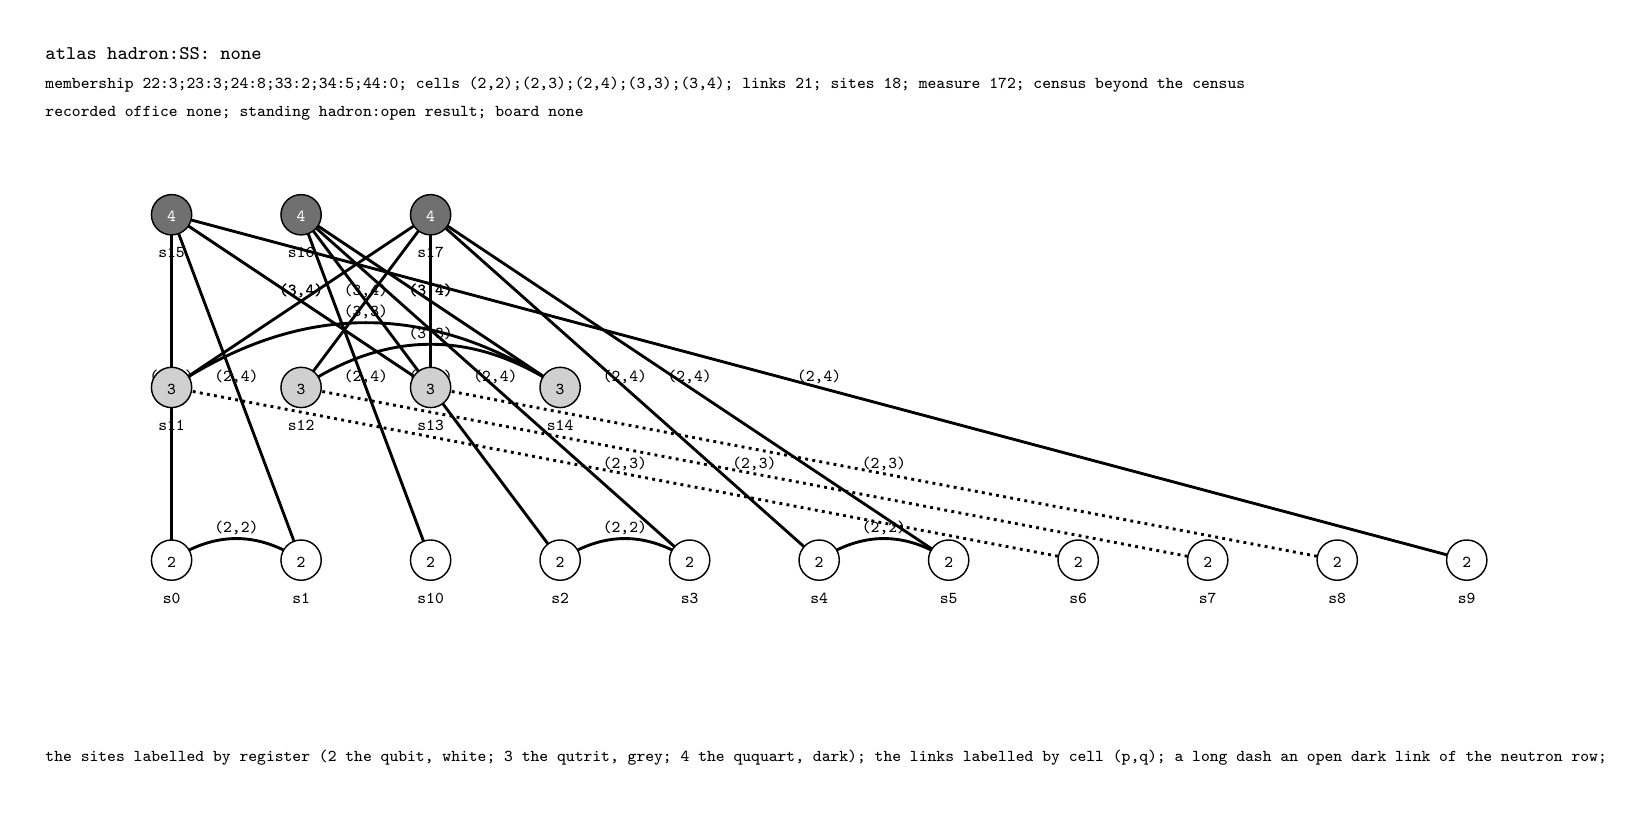
\begin{tikzpicture}[x=0.52pt,y=-0.52pt,baseline]
\clip (0,0) rectangle (1100,540);
\fill[white] (0,0) rectangle (1100,540);
\node[anchor=base west,inner sep=0pt,text=black,font=\fontsize{6.76}{8.112}\selectfont\ttfamily] at (12,22) {atlas hadron:SS: none};
\node[anchor=base west,inner sep=0pt,text=black,font=\fontsize{6.24}{7.488}\selectfont\ttfamily] at (12,42) {membership 22:3;23:3;24:8;33:2;34:5;44:0; cells (2,2);(2,3);(2,4);(3,3);(3,4); links 21; sites 18; measure 172; census beyond the census};
\node[anchor=base west,inner sep=0pt,text=black,font=\fontsize{5.72}{6.864}\selectfont\ttfamily] at (12,62) {recorded office none; standing hadron:open result; board none};
\draw[draw=black,line width=1.04pt] (100,370) -- (100,130);
\node[anchor=base,inner sep=0pt,text=black,font=\fontsize{5.72}{6.864}\selectfont\ttfamily] at (100,246) {(2,4)};
\draw[draw=black,line width=1.04pt] (100,370) .. controls (130,350) and (160,350) .. (190,370);
\node[anchor=base,inner sep=0pt,text=black,font=\fontsize{5.72}{6.864}\selectfont\ttfamily] at (145,351) {(2,2)};
\draw[draw=black,line width=1.04pt] (190,370) -- (100,130);
\node[anchor=base,inner sep=0pt,text=black,font=\fontsize{5.72}{6.864}\selectfont\ttfamily] at (145,246) {(2,4)};
\draw[draw=black,line width=1.04pt] (280,370) -- (190,130);
\node[anchor=base,inner sep=0pt,text=black,font=\fontsize{5.72}{6.864}\selectfont\ttfamily] at (235,246) {(2,4)};
\draw[draw=black,line width=1.04pt] (100,250) .. controls (190,190) and (280,190) .. (370,250);
\node[anchor=base,inner sep=0pt,text=black,font=\fontsize{5.72}{6.864}\selectfont\ttfamily] at (235,201) {(3,3)};
\draw[draw=black,line width=1.04pt] (100,250) -- (280,130);
\node[anchor=base,inner sep=0pt,text=black,font=\fontsize{5.72}{6.864}\selectfont\ttfamily] at (190,186) {(3,4)};
\draw[draw=black,line width=1.04pt,dash pattern=on 1.04pt off 1.56pt] (100,250) -- (730,370);
\node[anchor=base,inner sep=0pt,text=black,font=\fontsize{5.72}{6.864}\selectfont\ttfamily] at (415,306) {(2,3)};
\draw[draw=black,line width=1.04pt] (190,250) .. controls (250,210) and (310,210) .. (370,250);
\node[anchor=base,inner sep=0pt,text=black,font=\fontsize{5.72}{6.864}\selectfont\ttfamily] at (280,216) {(3,3)};
\draw[draw=black,line width=1.04pt] (190,250) -- (280,130);
\node[anchor=base,inner sep=0pt,text=black,font=\fontsize{5.72}{6.864}\selectfont\ttfamily] at (235,186) {(3,4)};
\draw[draw=black,line width=1.04pt,dash pattern=on 1.04pt off 1.56pt] (190,250) -- (820,370);
\node[anchor=base,inner sep=0pt,text=black,font=\fontsize{5.72}{6.864}\selectfont\ttfamily] at (505,306) {(2,3)};
\draw[draw=black,line width=1.04pt] (280,250) -- (100,130);
\node[anchor=base,inner sep=0pt,text=black,font=\fontsize{5.72}{6.864}\selectfont\ttfamily] at (190,186) {(3,4)};
\draw[draw=black,line width=1.04pt] (280,250) -- (280,130);
\node[anchor=base,inner sep=0pt,text=black,font=\fontsize{5.72}{6.864}\selectfont\ttfamily] at (280,186) {(3,4)};
\draw[draw=black,line width=1.04pt,dash pattern=on 1.04pt off 1.56pt] (280,250) -- (910,370);
\node[anchor=base,inner sep=0pt,text=black,font=\fontsize{5.72}{6.864}\selectfont\ttfamily] at (595,306) {(2,3)};
\draw[draw=black,line width=1.04pt] (370,250) -- (190,130);
\node[anchor=base,inner sep=0pt,text=black,font=\fontsize{5.72}{6.864}\selectfont\ttfamily] at (280,186) {(3,4)};
\draw[draw=black,line width=1.04pt] (100,130) -- (1000,370);
\node[anchor=base,inner sep=0pt,text=black,font=\fontsize{5.72}{6.864}\selectfont\ttfamily] at (550,246) {(2,4)};
\draw[draw=black,line width=1.04pt] (190,130) -- (370,370);
\node[anchor=base,inner sep=0pt,text=black,font=\fontsize{5.72}{6.864}\selectfont\ttfamily] at (280,246) {(2,4)};
\draw[draw=black,line width=1.04pt] (190,130) -- (460,370);
\node[anchor=base,inner sep=0pt,text=black,font=\fontsize{5.72}{6.864}\selectfont\ttfamily] at (325,246) {(2,4)};
\draw[draw=black,line width=1.04pt] (280,130) -- (550,370);
\node[anchor=base,inner sep=0pt,text=black,font=\fontsize{5.72}{6.864}\selectfont\ttfamily] at (415,246) {(2,4)};
\draw[draw=black,line width=1.04pt] (280,130) -- (640,370);
\node[anchor=base,inner sep=0pt,text=black,font=\fontsize{5.72}{6.864}\selectfont\ttfamily] at (460,246) {(2,4)};
\draw[draw=black,line width=1.04pt] (370,370) .. controls (400,350) and (430,350) .. (460,370);
\node[anchor=base,inner sep=0pt,text=black,font=\fontsize{5.72}{6.864}\selectfont\ttfamily] at (415,351) {(2,2)};
\draw[draw=black,line width=1.04pt] (550,370) .. controls (580,350) and (610,350) .. (640,370);
\node[anchor=base,inner sep=0pt,text=black,font=\fontsize{5.72}{6.864}\selectfont\ttfamily] at (595,351) {(2,2)};
\filldraw[fill=white,draw=black,line width=0.52pt] (100,370) circle (14);
\node[anchor=base,inner sep=0pt,text=black,font=\fontsize{6.24}{7.488}\selectfont\ttfamily] at (100,375) {2};
\node[anchor=base,inner sep=0pt,text=black,font=\fontsize{5.72}{6.864}\selectfont\ttfamily] at (100,400) {s0};
\filldraw[fill=white,draw=black,line width=0.52pt] (190,370) circle (14);
\node[anchor=base,inner sep=0pt,text=black,font=\fontsize{6.24}{7.488}\selectfont\ttfamily] at (190,375) {2};
\node[anchor=base,inner sep=0pt,text=black,font=\fontsize{5.72}{6.864}\selectfont\ttfamily] at (190,400) {s1};
\filldraw[fill=white,draw=black,line width=0.52pt] (280,370) circle (14);
\node[anchor=base,inner sep=0pt,text=black,font=\fontsize{6.24}{7.488}\selectfont\ttfamily] at (280,375) {2};
\node[anchor=base,inner sep=0pt,text=black,font=\fontsize{5.72}{6.864}\selectfont\ttfamily] at (280,400) {s10};
\filldraw[fill={rgb,255:red,208;green,208;blue,208},draw=black,line width=0.52pt] (100,250) circle (14);
\node[anchor=base,inner sep=0pt,text=black,font=\fontsize{6.24}{7.488}\selectfont\ttfamily] at (100,255) {3};
\node[anchor=base,inner sep=0pt,text=black,font=\fontsize{5.72}{6.864}\selectfont\ttfamily] at (100,280) {s11};
\filldraw[fill={rgb,255:red,208;green,208;blue,208},draw=black,line width=0.52pt] (190,250) circle (14);
\node[anchor=base,inner sep=0pt,text=black,font=\fontsize{6.24}{7.488}\selectfont\ttfamily] at (190,255) {3};
\node[anchor=base,inner sep=0pt,text=black,font=\fontsize{5.72}{6.864}\selectfont\ttfamily] at (190,280) {s12};
\filldraw[fill={rgb,255:red,208;green,208;blue,208},draw=black,line width=0.52pt] (280,250) circle (14);
\node[anchor=base,inner sep=0pt,text=black,font=\fontsize{6.24}{7.488}\selectfont\ttfamily] at (280,255) {3};
\node[anchor=base,inner sep=0pt,text=black,font=\fontsize{5.72}{6.864}\selectfont\ttfamily] at (280,280) {s13};
\filldraw[fill={rgb,255:red,208;green,208;blue,208},draw=black,line width=0.52pt] (370,250) circle (14);
\node[anchor=base,inner sep=0pt,text=black,font=\fontsize{6.24}{7.488}\selectfont\ttfamily] at (370,255) {3};
\node[anchor=base,inner sep=0pt,text=black,font=\fontsize{5.72}{6.864}\selectfont\ttfamily] at (370,280) {s14};
\filldraw[fill={rgb,255:red,112;green,112;blue,112},draw=black,line width=0.52pt] (100,130) circle (14);
\node[anchor=base,inner sep=0pt,text=white,font=\fontsize{6.24}{7.488}\selectfont\ttfamily] at (100,135) {4};
\node[anchor=base,inner sep=0pt,text=black,font=\fontsize{5.72}{6.864}\selectfont\ttfamily] at (100,160) {s15};
\filldraw[fill={rgb,255:red,112;green,112;blue,112},draw=black,line width=0.52pt] (190,130) circle (14);
\node[anchor=base,inner sep=0pt,text=white,font=\fontsize{6.24}{7.488}\selectfont\ttfamily] at (190,135) {4};
\node[anchor=base,inner sep=0pt,text=black,font=\fontsize{5.72}{6.864}\selectfont\ttfamily] at (190,160) {s16};
\filldraw[fill={rgb,255:red,112;green,112;blue,112},draw=black,line width=0.52pt] (280,130) circle (14);
\node[anchor=base,inner sep=0pt,text=white,font=\fontsize{6.24}{7.488}\selectfont\ttfamily] at (280,135) {4};
\node[anchor=base,inner sep=0pt,text=black,font=\fontsize{5.72}{6.864}\selectfont\ttfamily] at (280,160) {s17};
\filldraw[fill=white,draw=black,line width=0.52pt] (370,370) circle (14);
\node[anchor=base,inner sep=0pt,text=black,font=\fontsize{6.24}{7.488}\selectfont\ttfamily] at (370,375) {2};
\node[anchor=base,inner sep=0pt,text=black,font=\fontsize{5.72}{6.864}\selectfont\ttfamily] at (370,400) {s2};
\filldraw[fill=white,draw=black,line width=0.52pt] (460,370) circle (14);
\node[anchor=base,inner sep=0pt,text=black,font=\fontsize{6.24}{7.488}\selectfont\ttfamily] at (460,375) {2};
\node[anchor=base,inner sep=0pt,text=black,font=\fontsize{5.72}{6.864}\selectfont\ttfamily] at (460,400) {s3};
\filldraw[fill=white,draw=black,line width=0.52pt] (550,370) circle (14);
\node[anchor=base,inner sep=0pt,text=black,font=\fontsize{6.24}{7.488}\selectfont\ttfamily] at (550,375) {2};
\node[anchor=base,inner sep=0pt,text=black,font=\fontsize{5.72}{6.864}\selectfont\ttfamily] at (550,400) {s4};
\filldraw[fill=white,draw=black,line width=0.52pt] (640,370) circle (14);
\node[anchor=base,inner sep=0pt,text=black,font=\fontsize{6.24}{7.488}\selectfont\ttfamily] at (640,375) {2};
\node[anchor=base,inner sep=0pt,text=black,font=\fontsize{5.72}{6.864}\selectfont\ttfamily] at (640,400) {s5};
\filldraw[fill=white,draw=black,line width=0.52pt] (730,370) circle (14);
\node[anchor=base,inner sep=0pt,text=black,font=\fontsize{6.24}{7.488}\selectfont\ttfamily] at (730,375) {2};
\node[anchor=base,inner sep=0pt,text=black,font=\fontsize{5.72}{6.864}\selectfont\ttfamily] at (730,400) {s6};
\filldraw[fill=white,draw=black,line width=0.52pt] (820,370) circle (14);
\node[anchor=base,inner sep=0pt,text=black,font=\fontsize{6.24}{7.488}\selectfont\ttfamily] at (820,375) {2};
\node[anchor=base,inner sep=0pt,text=black,font=\fontsize{5.72}{6.864}\selectfont\ttfamily] at (820,400) {s7};
\filldraw[fill=white,draw=black,line width=0.52pt] (910,370) circle (14);
\node[anchor=base,inner sep=0pt,text=black,font=\fontsize{6.24}{7.488}\selectfont\ttfamily] at (910,375) {2};
\node[anchor=base,inner sep=0pt,text=black,font=\fontsize{5.72}{6.864}\selectfont\ttfamily] at (910,400) {s8};
\filldraw[fill=white,draw=black,line width=0.52pt] (1000,370) circle (14);
\node[anchor=base,inner sep=0pt,text=black,font=\fontsize{6.24}{7.488}\selectfont\ttfamily] at (1000,375) {2};
\node[anchor=base,inner sep=0pt,text=black,font=\fontsize{5.72}{6.864}\selectfont\ttfamily] at (1000,400) {s9};
\node[anchor=base west,inner sep=0pt,text=black,font=\fontsize{5.72}{6.864}\selectfont\ttfamily] at (12,510) {the sites labelled by register (2 the qubit, white; 3 the qutrit, grey; 4 the ququart, dark); the links labelled by cell (p,q); a long dash an open dark link of the neutron row; a short dash a docked link at the rule R1};
\end{tikzpicture}\end{adjustbox}
\caption{\texttt{SS of the hadron row}, hadron row body: 18 sites, 21 links, the measure 172; the links at the cells (2,2), (2,3), (2,4), (3,3), (3,4); the membership 22:3; 23:3; 24:8; 33:2; 34:5; 44:0; 3 docked links at the rule R1 (s6-s11; s7-s12; s8-s13); beyond the census of the six cells. Drawn at the anatomy atlas as its web, the sites labeled by register and the links by cell, from the hadron spectroscopy at the cap sinks.}\label{fig:VII-6-D540002-ss-670447}
\begin{center}\footnotesize\begin{adjustbox}{max width=\linewidth}\begin{tabular}{p{0.26\textwidth}p{0.68\textwidth}}\toprule
recorded office (the slot-count row) & no read of this body at the slot-count row \\
mass register (the mass-register row) & no read of this body at the mass-register row \\
\bottomrule\end{tabular}\end{adjustbox}\end{center}
\end{figure}
\end{chconditional}
\chstanding{conditional theorem}
\chdeps{Definitions 1.1 to 1.6, Theorem 172.1 and Open result 172.2, Theorems 174.1 and 174.2 and Open result 174.3 and Open results 245.1 and 245.2, Theorem 245.3, Open results 245.4 to 245.8 and Theorem 245.9}{Open result 178.1, Open result 179.1, Open result 180.1, Theorems 224.1 to 224.3 and Open result 224.4 and Open result 260.1}
The box takes the two nucleon stars with their free docks and lets the pairing move join them. The webs it can no longer act on are listed, and that list, up to eight stars, is what the compendium calls the hadron spectrum.
\begin{chconditional}[The mixed composition, the meson apparatus and the corollaries]\label{box:VII-6-hadron-spectrum-and-the-mesons:2}
Under their parents, the register of the common support, sixteen at every qutrit-qubit dock and eighty-one at every qutrit-qutrit leg and junction reading, is derived at the fourteen docks and the twelve legs of the six docked quark bodies and the two nucleon stars as one register at each reading, so the mixed composition at the eight bodies is defined at the adopted register in one rule; every meson measurement of the table, eleven at the quark and meson rows, is built from the roster cores as a joined web and joined to its apparatus at the hosts of the construction, the measuring body and the measured object an exact web in every case and a value nowhere; and the hadron and nuclear corollaries at the pairing move stand with six gated entries.
\end{chconditional}
\chstanding{conditional theorems, three}
\chdeps{Definitions 1.1 to 1.6, Theorem 172.1 and Open result 172.2, Theorems 174.1 and 174.2 and Open result 174.3 and Open results 245.1 and 245.2, Theorem 245.3, Open results 245.4 to 245.8 and Theorem 245.9}{Open result 178.1, Open result 179.1, Open result 180.1, Theorems 224.1 to 224.3 and Open result 224.4 and Open result 260.1}
The second box gathers the three theorems beside the spectrum.
\begin{chwall}[The direct sum at the deuteron]\label{box:VII-6-hadron-spectrum-and-the-mesons:3}
The direct two-exchange sum at the deuteron web, the two stars paired at the up leaves at one dark qutrit-qutrit link, meets the deuteron office of the earlier result at neither binding entry, while the meson web direct sum is defined as an exact object at every one of the twenty-one pairings of two qutrit cores admitted at the valence bound.
\end{chwall}
\chstanding{open result, built and not closed}
\chdeps{Definitions 1.1 to 1.6, Theorem 172.1 and Open result 172.2, Theorems 174.1 and 174.2 and Open result 174.3 and Open results 245.1 and 245.2, Theorem 245.3, Open results 245.4 to 245.8 and Theorem 245.9}{Open result 178.1, Open result 179.1, Open result 180.1, Theorems 224.1 to 224.3 and Open result 224.4 and Open result 260.1}
The third box names the one reading that parts.
\begin{chbridge}
What this chapter calls the saturated joined webs the literature calls the nuclei, the chain of two neutron stars a dineutron, the web of two neutrons and two protons the alpha particle, the one-link pairing of two quark cores a meson and the pairing move the nuclear binding. The correspondence is by name; the pairing move does not reach the deuteron as a sink.
\end{chbridge}
\begin{chproof}[census]
The premises are the saturation of chapter 1-5, a theorem, the strong coupling of chapter 7-2 and the nucleon star of chapter 7-3, theorems. The chain from the axiom to this chapter is seven chapters long. The set counted is the set of joined webs the pairing move builds from the two stars at their pairable docks, enumerated at every star count from one to four at the dock level and from five to eight at the star level as labeled arrangements, and the property tested is whether the web is a sink of the pairing move, every dock of every star paired. By kind. At one star no sink, the proton star at two free docks and the neutron star at one. At two stars one sink, the chain of two neutrons. At three stars two, the chain neutron-proton-neutron and the proton cycle. At four stars two, the chain of two protons between two neutrons and the proton cycle, and at every count from five to eight two, the chain of proton stars capped by two neutron stars and the cycle of proton stars,
\begin{equation}
14 = 0 + 1 + 2 + 2 + 2 + 2 + 2 + 2 + 1 ,
\end{equation}
with the two-star double pairing beside at the multiple reading. The smallest case is the chain of two neutrons, 30 sites and 33 links, four of genre (2,2), six of (2,3), twelve of (2,4), seven of (3,3) and four of (3,4), its two docks paired and none free, the register 16 at the dock face and 81 at the port face. The web of two neutrons and two protons has 52 sites and 57 links with its six docks all paired, the unique sink at two and two, and the deuteron, the path of one neutron and one proton, is a sink not, its proton dock free. The saturation of the roster is reached at no count to the bound, a count and no claim beyond it.

The site-level isomorphism kinds of the earlier result equal the star-level words at every composition up to four stars at all sixteen label readings, the catalog re-met at 53 kinds with 9 shared groups. The mesons beside are the one-link pairings of the six docked quark bodies at one dark (3,3) link between their cores, a body with its own copy admitted and a body of another kind admitted not at the first reading. For the second box the register of the common support is derived at the fourteen docks and twelve legs as one register at each reading, the eleven meson measurements are built as joined webs with their apparatus, and the corollaries stand at their six gated entries.

\emph{Check.} The sink test was carried at both multiplicity readings, the sinks within a web beside the sinks of the pairing, with the deuteron and helium-3 checked by name as sinks never and the triton as a sink. The result was reproduced by an independent route, two engines at every capture byte for byte, its five counter-tests at their pinned letters and its controls the same at both routes.
The direct sum at the deuteron meets the deuteron office at neither binding entry, and the six gated entries of the corollary theorem stand gated. The nuclear rows at the joined seeded web are the matter of chapter 9-7.
\chcert{14}
\end{chproof}
\label{chend:VII-6-hadron-spectrum-and-the-mesons}
\section{The heavy-flavor sinks at the hadron rows}\label{mod:VII-6-D539921-w-hfhd}
\begin{chwall}[The heavy-flavor sinks at the hadron rows]\label{box:VII-6-D539921-w-hfhd:1}
This result is conditional on the parents at their grades, the decay board an instrument and the hadron-spectrum, bound-respecting, proton-web and rep-census entries read at their grades, the composition riding the lowest grade in its chain. Under the axiom text, the dock rule and the parent results, every heavy sink carries its office of the form the item words, the cap of the (2,3) genre squared multiplied by nine to the exponent of its dressing, 74183769, 667653921, 74183769 and 8242641 at the charm, strange, bottom and top sinks, and the current-mass entries of the board are of another kind, the quark words docked bodies without a junction leg and the sinks saturated webs with junction legs, their webs and offices parting at four of four; but no heavy sink is placed at a hadron row of the decay board or at a spectrum row by its structure at the reading adopted, the dock count, the arm count at the center-and-hub-removed reading and the hub count equal to no row web at zero of four: the charm sink at two docks, two arms and two hubs, the strange and the top sinks at three, three and three, the bottom sink at two, two and three, against the proton row at three, three and one, the neutron row at three, three and two and the roster webs at three docks per star, the twenty-seven meson and baryon rows of the decay board carrying no sink at that depth; the heavy sinks match the one-link meson pairings of the hadron-spectrum entry beside, the charm sink the charm word paired with itself, at the center-and-hub-removed reading alone, printed beside; the first parting the charm sink.
The first face, each heavy sink placed at a hadron row of the decay board or the spectrum rows by its structure with its office beside the row and the current-mass entries typed as a parting of kind, reads no, the sinks placed zero of four while the kind typing parts at four of four; the second face, a heavy sink placed at no hadron row named, reads yes at the first parting of the item order, the charm sink. Open is the placement of the heavy sinks at the hadron rows: their structures match no row web at the reading adopted, and they match meson pairings at one reading beside alone.
\end{chwall}
\chstanding{an open result}
\chdeps{Definitions 1.1 to 1.6 and Theorems 177.1 and 177.2 and Open result 177.3}{no theorem beyond it at this release}
The four heavy sinks, the first saturated sinks reached at each heavy flavor, carry offices of one form, the hadron cap squared multiplied by a power of nine fixed by the dressing. The question is whether each sits at a hadron row, of the decay board or of the spectrum, when both are described by the same triple, the number of docks, the number of arms once the center and the hubs are removed, and the number of hubs. None does: the proton row has one hub and three docks, the neutron row two hubs and three docks, the spectrum webs three docks per star, while the charm sink has two of each, and the twenty-seven meson and baryon rows of the board carry no sink web at all. The quark words of the current-mass entries are a different kind of object, docked bodies with no junction leg, so the heavy sinks are neither the hadron rows nor the quarks, and only at one reading beside do they match meson pairings.
\begin{chbridge}
The heavy quarks of the Standard Model, charm, strange, bottom and top, are confined into mesons and baryons whose masses are set by the strong interaction and the quark masses together, the quark masses themselves scheme-dependent parameters rather than observable rest masses \cite{Gasser1982,Peskin1995}. The correspondence is by name.
\end{chbridge}
\begin{chproof}[exhaustive census with its exact part]
The premises of this derivation are the axiom and the six definitions of chapter~\ref{mod:FRAMEWORK}, the hadron spectrum and the mesons of the present chapter, a theorem, the quark content and flavor of chapter~\ref{mod:VII-7-quark-content-and-flavour}, a theorem, the proton as a seeded sink of chapter~\ref{mod:VII-4-proton-as-a-seeded-sink}, a theorem, the body-alone office rule of chapter~\ref{mod:VIII-2-body-alone-office-rule}, a theorem, and the decay board of chapter~\ref{mod:IX-1-decay-as-the-forward-edge-of-a-non-sink-the-move-graph-of-the-hub-step}, an instrument. The chain of premises runs back to the axiom through those chapters, and the longest such chain in this compendium is twelve chapters long.
\textit{The exact part.} The office of each heavy sink is the cap of the (2,3) genre, 319 at the cap census, squared and multiplied by nine to the exponent of its dressing,
\begin{equation} \adjustbox{max width=\dimexpr\linewidth-3em\relax}{$\displaystyle \Omega_{c} = 319^{2}\cdot 9^{3} = 74183769, \quad \Omega_{s} = 319^{2}\cdot 9^{4} = 667653921, \quad \Omega_{b} = 319^{2}\cdot 9^{3} = 74183769, \quad \Omega_{t} = 319^{2}\cdot 9^{2} = 8242641,$} \end{equation}
each a cell of the quark-offices entry re-met by locator at four of four, exact of the form at four of four. The structure of a web is its dock count by the dock rule, the pendant end the smaller end of the genre, its arm count at the center-and-hub-removed reading and its hub count by the hub rule, and a sink is placed at a row when its triple equals the triple of the row web. The figure draws the triple of the charm sink beside that of the proton row.
\textit{The census.} By exhaustive enumeration of the four heavy sinks against the forty-three hadron rows, the twenty-nine rows of the decay board, the proton row at the sink of the bound-respecting entry with eight sites, nine links and the triple three, three, one, the neutron row at the proton-web seed with thirteen sites, sixteen links and the triple three, three, two, and the twenty-seven meson and baryon rows at no sink at that depth, their structure undefined, together with the fourteen roster webs of the hadron spectrum re-met at their sites, links and genre census at fourteen of fourteen, from the triple six, four, two at two stars to twenty-four, seventeen, ten at eight: the property tested is equality of the triples; the counts are placed at zero of four at the reading adopted, the charm sink at two, two, two, the strange and the top at three, three, three and the bottom at two, two, three equal to no row; printed beside, at the whole triple the charm sink equals the meson pairing of the charm word with itself and the strange and top sinks their pairings, at the center-and-hub-removed reading alone. The kind typing: each sink is a saturated web carrying junction legs, three at the charm, two at the strange, three at the bottom and three at the top, and the docked quark word of the flavor carries none, their webs parting at four of four, fifteen sites against six, eighteen against ten, sixteen against thirteen and seventeen against nine, and their offices parting at four of four, 74183769 against 101761, 667653921 against 8242641, 74183769 against 8242641 and 8242641 against 101761. The smallest case is the charm sink against the proton row, two docks against three.
\textit{The check.} The counter-tests alter the construction singly and read what moves. Reading the charm sink at the library copy moves its triple, forty-seven cells. Striking the first hub of the charm sink moves its hub count, twenty-eight cells. Reading the placement at the hub axis alone places the charm sink at the neutron row, thirty-four cells. Striking the text unmeets the gate. Each alteration moves the cells it names, four of four. The result was reproduced by an independent route, two engines built apart, a map-and-set route against the second route, equal at every cell, with the fourteen controls the same and the office runs equal at ten of ten.
\chcert{43}
\begin{figure}[h]\centering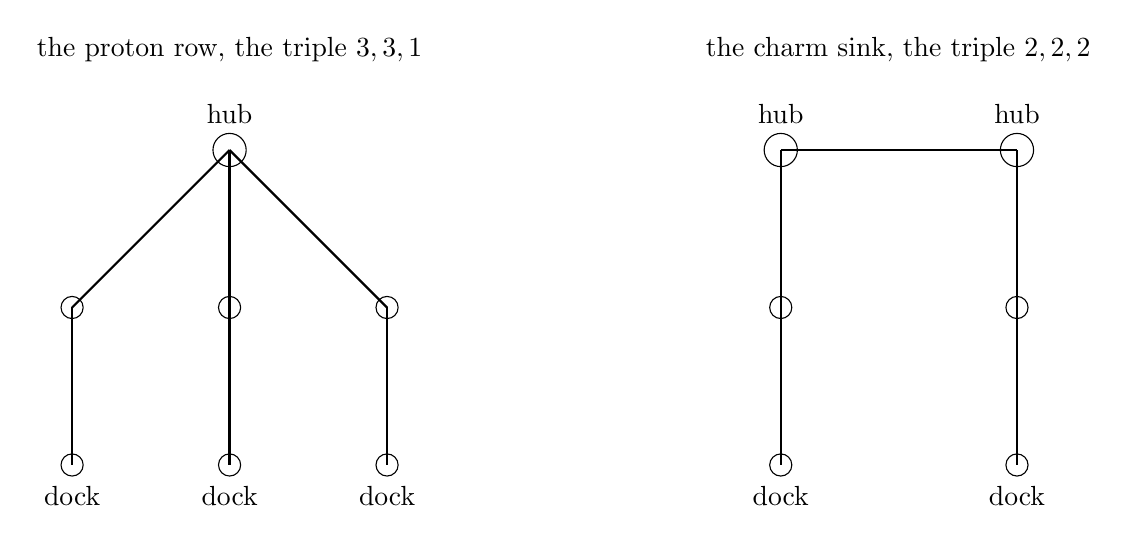
\begin{tikzpicture}[scale=1]
\filldraw[fill=white] (0,0) circle (6pt) node[above=6pt] {hub};
\foreach \a in {-2,0,2} {\filldraw[fill=white] (\a,-2) circle (4pt); \draw[thick] (0,0) -- (\a,-2); \filldraw[fill=white] (\a,-4) circle (4pt) node[below=4pt] {dock}; \draw[thick] (\a,-2) -- (\a,-4);}
\node at (0,1) [above] {the proton row, the triple $3, 3, 1$};
\filldraw[fill=white] (7,0) circle (6pt) node[above=6pt] {hub}; \filldraw[fill=white] (10,0) circle (6pt) node[above=6pt] {hub};
\draw[thick] (7,0) -- (10,0);
\foreach \a in {7,10} {\filldraw[fill=white] (\a,-2) circle (4pt); \draw[thick] (\a,0) -- (\a,-2); \filldraw[fill=white] (\a,-4) circle (4pt) node[below=4pt] {dock}; \draw[thick] (\a,-2) -- (\a,-4);}
\node at (8,1) [above, xshift=14pt] {the charm sink, the triple $2, 2, 2$};
\end{tikzpicture}\caption{The structure triples compared: the proton row with three docks, three arms and one hub, and the charm sink with two docks, two arms and two hubs, drawn as schematics of their counts.}\end{figure}
\end{chproof}
\section{Hadron spectroscopy at the cap sinks}\label{mod:VII-6-D540002-w-hadx}
\begin{chwall}[Hadron spectroscopy at the cap sinks]\label{box:VII-6-D540002-w-hadx:1}
This result is conditional on the wave budget of its source and on the parent results at their grades, the open results among them read at their grades. The first sink with no first power is named with its cells: the gluon-only sink 94 of the proton-web saturation at wave two, the docks zero at the census typing, every (2,3) link of it pendant at its qutrit end, fourteen sites, eighteen links, the measure 143, the entry dock none and the first power no hub at both engines under the dock rule. The open result face: at the dock rule and the typing adopted every excited sink with a pendant-qubit dock carries a first power 319 multiplied by a power of three, 234 of 276, the ladders at six and three distinct first powers with no read at the swapped cap, and every excited sink without one carries none, 42 of 276, the four gluon-only sinks of the three-quark saturation and the thirty-eight dock-free cap sinks of the two-quark saturation; both faces printed at every class.
The first face, every excited sink of the two saturations within the budget a cell with a first power by the segment theorem, reads no at 234 of 276; the second face, the first sink with no first power named with its cells, reads yes at the sink 94. Open is the first power at the dock-free sinks: a read enters a sink at a dock alone, the pendant qubit of a (2,3) link, and a sink with no such link is entered nowhere.
\end{chwall}
\chstanding{an open result}
\chdeps{Definitions 1.1 to 1.6 and Theorems 177.1 and 177.2 and Open result 177.3}{no theorem beyond it at this release}
The excited states of the hadron spectrum are read here as the saturated sinks beyond the ground state of two saturations, the three-quark saturation seeded at the proton web, 181 sinks within the wave budget of the entry, and the two-quark saturation at the pion web, 96 cap sinks. The first power of a sink by the segment theorem is read by entering at its first dock, the pendant qubit of a (2,3) link, capping the entered link at the cap of the genre, 319, stopping at the first hub and dressing the entry segment by three for every in-leg left unpassed. Every sink that has a dock gets a first power of the form 319 multiplied by a power of three, and the first powers fall on ladders, six distinct values in the three-quark saturation and three in the two-quark, with exact ratios to the ground states. But a sink whose (2,3) links are all pendant at the qutrit end has no dock, no entry and no first power, and the open result names the first such sink, a gluon-only sink of the proton-web saturation.
\begin{chbridge}
Hadron spectroscopy lists the excited states of mesons and baryons on Regge trajectories, their masses rising with the spin and the radial excitation, and the glueballs, bound states of gluons alone, are predicted by the theory and not yet identified \cite{Chew1962,Mathieu2009}. The correspondence is by name.
\end{chbridge}
\begin{chproof}[exhaustive census with its exact part]
The premises of this derivation are the axiom and the six definitions of chapter~\ref{mod:FRAMEWORK}, the hadron spectrum and the mesons of the present chapter, a theorem, the proton as a seeded sink of chapter~\ref{mod:VII-4-proton-as-a-seeded-sink}, a theorem, the quark content and flavor of chapter~\ref{mod:VII-7-quark-content-and-flavour}, a theorem, and the first power as the sum over the segments of the read of chapter~\ref{mod:VIII-1-mass-unit-and-the-first-power}, a theorem. The chain of premises runs back to the axiom through those chapters, and the longest such chain in this compendium is twelve chapters long.
\textit{The exact part.} The first power of a sink by the segment theorem is the cap of the entered genre, 319 at the (2,3) genre, multiplied by three to the number of in-legs the read leaves unpassed at the first hub,
\begin{equation} S_{1} = 319\cdot 3^{u}, \qquad \frac{S_{1}}{S_{1}(\text{ground})} \in \Big\{\tfrac{1}{9},\ \tfrac{1}{3},\ 1,\ 3,\ 9,\ 243\Big\} \ \text{over } 2871 \ \text{and} \ \{1,\ 3,\ 9\} \ \text{over } 319, \end{equation}
the ground state of the three-quark saturation at $2871 = 319\cdot 9$ and of the two-quark saturation at $319$, every ratio an exact rational reduced at two routes, 234 of 234, and the ratios over the electron unit 67 alike. The figure draws a (2,3) link pendant at its qubit end, a dock, beside one pendant at its qutrit end, which is no dock.
\textit{The census.} By exhaustive enumeration of the 276 excited sinks, the 180 sinks beyond the ground state of the three-quark saturation within the wave budget, waves zero to two, and the 96 cap sinks of the two-quark saturation beyond its first, each listed at its anatomy equal to its sites, links and measure by locator, 279 of 279 reads the same: the property tested at each sink is whether a read enters it at a dock, a (2,3) link pendant at its qubit end, so that the segment theorem gives a first power; the counts by class are a first power defined at 234 of 276, 176 of 180 three-quark and 58 of 96 two-quark, and no hub at 42 of 276, every one typed dock-free by locator, the four gluon-only sinks 94, 111, 136 and 139 of the three-quark saturation and the 38 dock-free cap sinks of the pion web. The first parting element is the sink 94 at wave two, dark by the dock count and by the form, with fourteen sites, eighteen links, the measure 143, two hubs and the genre census (2,2) two, (2,3) four, (2,4) six, (3,3) three and (3,4) three, every (2,3) link pendant at its qutrit end, so the entry dock is none, the first power no hub and the office undefined. The smallest case worked is the ground state itself, the seed web of ten sites and twelve links at the measure 101, read at two roots equal.
\textit{The check.} The counter-tests alter the construction singly and read what moves. The four parent strikes at every root, the arm struck from the star sum, the flavor selection flipped, the charm sink read at the library copy and the text struck, move their named cells at twelve of twelve pieces. Striking the dock dimension to the qutrit enters sixteen sinks at the swapped cap 475 and moves 342 of 345 cells. Striking the typing to uncapped moves the ground office from 2871 to 747 and 261 of 551 cells. Each alteration moves the cells it names, fourteen of fourteen. The result was reproduced by an independent route, two engines built apart, the python route against the perl route, equal at every cell, with the twenty-five controls the same and the parent engines on their own image equal at twenty-two of twenty-two pairs.
\chcert{276}
\begin{figure}[h]\centering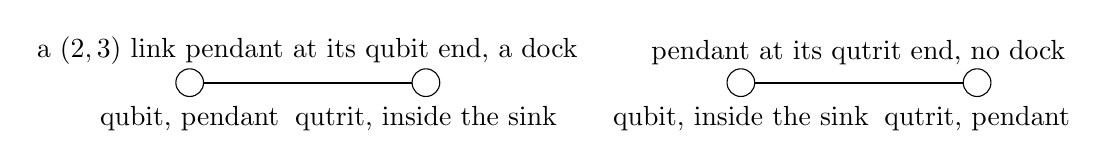
\begin{tikzpicture}[scale=1]
\draw[thick] (0,0) -- (3,0);
\filldraw[fill=white] (0,0) circle (5pt) node[below=5pt] {qubit, pendant};
\filldraw[fill=white] (3,0) circle (5pt) node[below=5pt] {qutrit, inside the sink};
\node at (1,0) [above=3pt, xshift=14pt] {a $(2,3)$ link pendant at its qubit end, a dock};
\draw[thick] (7,0) -- (10,0);
\filldraw[fill=white] (7,0) circle (5pt) node[below=5pt] {qubit, inside the sink};
\filldraw[fill=white] (10,0) circle (5pt) node[below=5pt] {qutrit, pendant};
\node at (8,0) [above=3pt, xshift=14pt] {pendant at its qutrit end, no dock};
\end{tikzpicture}\caption{The dock rule: a read enters a sink at the pendant qubit of a (2,3) link alone; the gluon-only sink 94 has four (2,3) links, every one pendant at its qutrit end, and so no entry.}\end{figure}
\end{chproof}
\section{The hadron offices from membership}\label{mod:VII-6-D543708-w-hdom}
\begin{chwall}[The hadron offices from membership]\label{box:VII-6-D543708-w-hdom:1}
The office formula at the junction register parts from the offices of the nucleon and the hadron sinks, the first parting the proton sink: the formula with its first-power bracket at the junction register of the share face at the dressing is met at zero of thirteen reads, the first parting the proton sink, its first power 729 against 2871, located at a count, the share-face register 81 against the cap 319 of the (2,3) genre, the Born count of the count law, at the dressing exponent two; the capped reads are met at the cap register with the closure zero, seven of thirteen, and the hub-count-two sinks at the dock-struck bracket, four of thirteen; the first face unmet at the reading adopted, the second face met with the first parting named with both cells; every cell an exact element of the field of root two and root three compared with nothing.
The first face, every established office of the nucleon and the hadron sinks met by the formula at the junction register, reads no, the formula met at zero of thirteen; the second face, the first parting named and located at a count, reads yes at the proton sink. Open is the first power of a hadron read as a formula in its membership counts: at the junction register of the share face the bracket gives 81 where the capped read of the nucleon gives 319, and the formula meets the capped reads only at the cap register and the hub-count-two sinks only at the dock-struck bracket.
\end{chwall}
\chstanding{an open result}
\chdeps{Definitions 1.1 to 1.6 and Theorems 177.1 and 177.2 and Open result 177.3}{no theorem beyond it at this release}
The office-as-a-formula entry of the mass chapter writes the office of a body in the six membership counts of its links by genre, with a first-power bracket and a closure at the counts, and this entry asks whether that formula, evaluated with the bracket at the junction register of the share face, re-meets the offices of the nucleon and of the hadron sinks. The junction register of the proton star is 81, the (3,3) register of its three junction legs at a share of one third each, and multiplied by the dressing at the exponent two it gives a first power of 729, while the office of the proton sink has the first power 2871, the cap 319 of the (2,3) genre multiplied by nine. The two part at one count, the share-face register against the cap, and the same parting stands at every nucleon read, while the capped reads are met if the cap register is used and the hub-count-two sinks if the dock-struck bracket is; the three hadron open results of the chapter are re-read as instances of the formula at a count.
\begin{chbridge}
The mass of a hadron is in the standard account the sum of its constituent masses and its binding, with the proton mass set almost entirely by the strong interaction among three light quarks joined at a color-singlet vertex \cite{Gasser1982,Peskin1995}. The correspondence is by name.
\end{chbridge}
\begin{chproof}[exact-cell derivation with its census]
The premises of this derivation are the axiom and the six definitions of chapter~\ref{mod:FRAMEWORK}, the hadron spectrum and the mesons of the present chapter, a theorem, the proton as a seeded sink of chapter~\ref{mod:VII-4-proton-as-a-seeded-sink}, a theorem, the nucleon structure and the form factor of chapter~\ref{mod:VII-3-nucleon-structure-and-the-form-factor}, a theorem, the body-alone office rule of chapter~\ref{mod:VIII-2-body-alone-office-rule}, a theorem, and the office as a formula in the membership counts of chapter~\ref{mod:VIII-1-mass-unit-and-the-first-power}, an open result. The chain of premises runs back to the axiom through those chapters, and the longest such chain in this compendium is twelve chapters long.
\textit{The exact part.} The proton sink carries the membership vector $(0, 3, 0, 3, 3, 0)$ over the genres (2,2), (2,3), (2,4), (3,3), (3,4) and (4,4), the struck vector $(0, 3, 0, 0, 0, 0)$, the dressing exponent two and the share-face register 81 at its junction site, a qutrit of degree three whose three (3,3) legs carry the share one third each, summing to one. The formula at the junction register gives the first power
\begin{equation} S_{1}^{\mathrm{formula}} = 81\cdot 3^{2} = 729 \qquad \text{against} \qquad S_{1}^{\mathrm{office}} = 319\cdot 9 = 2871 , \end{equation}
so the parting is located at one count, the share-face register 81 against the cap 319 at the dressing exponent two, and the formula cell, an element of the field with a sixteen-digit rational coordinate and a root-three coordinate printed at the table of the entry, parts from the office 8242641 of the proton sink. The figure draws the junction site of the proton star.
\textit{The census.} By exhaustive enumeration of the seventeen reads, the proton sink, the neutron through the deuteron and the strike-rule neutron, the proton star, the four heavy sinks, the four gluon-only sinks and the five hub-count-two sinks, each with its junction sites, its junction registers at the share face, the dock-struck reading and the hub-product reading, and its membership vector, re-met against the junction-star and census entries at every read: the property tested at each of the thirteen reads carrying an office is whether the formula at the junction register of the share face at the dressing, with the closure at the counts, equals the office; the counts are met at zero of thirteen at the reading adopted, the capped reads of the body-alone and heavy-flavor entries met at the cap register with the closure zero at seven of thirteen, and the hub-count-two sinks met at the dock-struck bracket with the closure at the counts at four of thirteen; the gluon-only sinks carry no office and are compared with nothing; the three hadron open results of the chapter are instances of the formula at a count at three of three, the gluon-only sink at the dock count, the heavy sinks at the dock and hub counts and the hub-count-two sink at the membership vectors. The smallest case is the proton sink worked above.
\textit{The check.} The counter-tests alter the construction singly and read what moves. Striking the first (3,3) leg at the first junction center moves the registers at every read with a junction site. Adding a (3,3) end to every membership vector moves the formula cells. Dropping the closure moves every read with a nonzero closure. Reading a word of the library with no junction, the docked top word, holds at the cells with its formula cell printed and compared with nothing. Striking the gate exits at both engines. Each alteration moves the cells it names, five of five. The result was reproduced by an independent route, two engines built apart, the explicit record-space route against the second route, equal at every cell, with the fifteen controls the same.
\chcert{17}
\begin{figure}[h]\centering\begin{tikzpicture}[scale=1]
\filldraw[fill=white] (0,0) circle (6pt) node[above=6pt] {the junction site, dimension 3, degree 3};
\foreach \a in {-3,0,3} {\filldraw[fill=white] (\a,-2) circle (5pt); \draw[thick] (0,0) -- (\a,-2);}
\node at (-2,-1) [left] {$(3,3)$, share $\tfrac{1}{3}$}; \node at (0,-1) [right] {$(3,3)$, share $\tfrac{1}{3}$}; \node at (2,-1) [right] {$(3,3)$, share $\tfrac{1}{3}$};
\node at (0,-3) [below] {the junction star of the proton, the share-face register $81$ against the cap $319$};
\end{tikzpicture}\caption{The junction site of the proton star with its three (3,3) legs at a share of one third each; the formula at its register gives the first power 729 where the capped read gives 2871.}\end{figure}
\end{chproof}
\par\medskip\noindent{\itshape The spectrum read, the next chapter reads what the hadrons are made of.}\label{narr:close:7-6}\par
\section{Quark content and flavour}\label{mod:VII-7-quark-content-and-flavour}
\chdesig{9-7}{7-7}{VII-7-quark-content-and-flavour}{VII-7-D539669-udao-t1}
\label{narr:open:7-7}Theorem~181.1 reads the quark register at the second-order junction read, Theorem~181.2 flavor as the rung name with the quark ladder, Open result~181.3 the five readings beside, Theorem~181.4 the quark ladder at the saturated sinks, and Theorem~181.5, a theorem, the quark offices as the star arm reads.
\begin{chconditional}[The quark register at the second-order junction read]\label{box:VII-7-quark-content-and-flavour:1}
Under its parents, the read engine run through every junction star at order two reads every leg with the entering link at the cut register, so the junction entry of a second read link is one exact object, eight at the cut reading, equal to the cut-reading bound at every one of the six quark bodies, and the share is the colour third, one third per leg; the junction tensor at the two-read junction of the down body equals the bounded tensor at the count ratio one third.
\end{chconditional}
\chstanding{conditional theorem}
\chdeps{Definitions 1.1 to 1.6, Theorem 171.1 and Open result 171.2, Theorems 174.1 and 174.2 and Open result 174.3 and Open results 241.1 and 241.2, Theorems 241.3 and 241.4 and Open results 241.5 to 241.7}{Theorem 27.1, Theorem 181.4, Theorem 181.5, Chapter 9-7 and Chapter 9-7}
The box reads each quark body as a star centered on its junction qutrit and finds that every leg of the star takes exactly one third of the read, the color third, and that the entry of a leg read at second order is one exact number equal to the bound.
\begin{chconditional}[Flavor as the rung name and the quark ladder]\label{box:VII-7-quark-content-and-flavour:2}
Under their parents, flavour is the rung name read at the corner: the three corner frames of the charged-lepton dark triangle at one, two and three hub legs equal the three residues of the adopted naming at every corner, the residue of the depth momentum read there; and the hub step applied at the up and down bodies with the junction legs kept at one and two steps gives the quark ladder, its hub counts and generation labels compared with the roster ladders.
\end{chconditional}
\chstanding{conditional theorems, two}
\chdeps{Definitions 1.1 to 1.6, Theorem 171.1 and Open result 171.2, Theorems 174.1 and 174.2 and Open result 174.3 and Open results 241.1 and 241.2, Theorems 241.3 and 241.4 and Open results 241.5 to 241.7}{Theorem 27.1, Theorem 181.4, Theorem 181.5, Chapter 9-7 and Chapter 9-7}
The second box gathers the two theorems on flavor, what names a generation, and how the heavier quarks are reached from the lighter by the hub step.
\begin{chwall}[The five readings beside]\label{box:VII-7-quark-content-and-flavour:3}
The slot-star register of the junction read and the vertex leg register are one object at a junction star whose other legs are unread and two objects at the star carrying a second read link, the whole 36 against the cut 24; the entry of a leg bounded by the share rule is one third of the pair-ket unit, 12 at the whole reading and 8 at the cut reading, parting at the two-read junction of the down quark; the six quark-body types are typed from the roster alone at six distinct arm signatures, but the typed count is not a first-order register count; the hub-leg cut is not the selection rule for quark flavour either, the twenty hub-leg cuts that change a count each losing one quark and gaining a quark pair; and the quark content as the set of the star reads at one arm parts at the lepton weight against the weight one with the colour.
\end{chwall}
\chstanding{open results, five, built and not closed}
\chdeps{Definitions 1.1 to 1.6, Theorem 171.1 and Open result 171.2, Theorems 174.1 and 174.2 and Open result 174.3 and Open results 241.1 and 241.2, Theorems 241.3 and 241.4 and Open results 241.5 to 241.7}{Theorem 27.1, Theorem 181.4, Theorem 181.5, Chapter 9-7 and Chapter 9-7}
The third box names the readings tried and parted.
\begin{chbridge}
What this chapter calls the color third the literature calls the color charge of a quark, the junction read the color-singlet projection and the rung name the generation number, the nearest objects. The correspondence is by name, and no quark mass is displayed here.
\end{chbridge}
\begin{chproof}[finite computation]
The premises are the moves of chapter 1-4, a definition, confinement of chapter 7-1 and the nucleon star of chapter 7-3, theorems. The chain from the axiom to this chapter is seven chapters long. The procedure. The input is the six quark bodies of the catalog with the first-order dock at each and the junction site of dimension 3, three junction stars (the down, the strange and the bottom) and three chain bodies (the up, the charm and the top), each leg typed read or unread by its genre. The enumeration runs the read engine through every star at order two at both polarities, the junction-center polarity and the larger-dimension polarity, the count law at every leg with the traceless dimensions at the far end and the center. The test compares the junction entry of a second read link with the bound. The aggregation forms the per-leg share. The smallest instance is one leg of a junction star, the share is the color third, the pair ket at dimension three flat at
\begin{equation}
\frac{1}{3}, \frac{1}{3}, \frac{1}{3}, \qquad \frac{1}{3} + \frac{1}{3} + \frac{1}{3} = 1 ,
\end{equation}
multiplied by the leg readout, at every (2,3) leg
\begin{equation}
\frac{79}{62208} + \frac{1}{1296}\sqrt{2} + \frac{7}{10368}\sqrt{3} + \frac{1}{20736}\sqrt{6} ,
\end{equation}
an exact element of the field of root two and root three, at 8 of 8 stars over 21 legs at both polarities. The junction entry at the cut reading is 8, equal to the bound at 6 of 6 bodies, and the up body at the first-order office $36/4489$ at the dock unit.

From the three corner frames of the charged-lepton dark triangle at one, two and three hub legs, by the residue of the depth momentum modulo three, we obtain the three residues of the adopted naming at every corner, flavor as the rung name. From the up and down bodies, by the hub step with the junction legs kept at one and two steps, we obtain the quark ladder with its hub counts and generation labels compared with the roster ladders. The five readings beside part at their named steps.

\emph{Check.} The first cut of this entry stood beyond the never-input gate and was set aside with its content confirmed at every part. The re-fire re-derived every cell at both engines. The result was reproduced by an independent route, two engines at every capture byte for byte, its five counter-tests at their pinned letters and its twelve controls the same at both routes.
The register at the junction read at its deciding reading, the bounded entry at the two-read junction, the selection rule for flavor and the content at an unequal far end stay open.
\chcert{21}
\end{chproof}
\label{chend:VII-7-quark-content-and-flavour}
\subsection{The quark ladder at the saturated sinks}\label{mod:VII-7-D536267-qlsk-t1}
\begin{chconditional}[The quark ladder at the saturated sinks]\label{box:VII-7-D536267-qlsk-t1:1}
Under its parents, the open results among them, the four heavy-flavour first powers, the strange, the charm, the bottom and the top, are outputs of the hub lowering at the saturated sinks, each a rank multiplied by a dressing: the first reached charm 147 by 81, strange 172 by 243, top 165 by 108 and bottom 171 by 324, with 19, 82, 51 and 87 distinct reached values per flavour, and the top-to-W ratio 891 at the first reached top a cell beside.
\end{chconditional}
\chstanding{conditional theorem}
\chdeps{Definitions 1.1 to 1.6 and Theorems 181.1 and 181.2 and Open result 181.3}{no theorem beyond it at this release}
The box reaches the four heavy quarks from the stable webs of the saturation by one move, the lowering of a hub, and reads the first power of each web reached as the product of a rank and a dressing. Every one of the four flavors is reached.
\begin{chbridge}
What this chapter calls the hub lowering at a sink the literature calls a flavor transition, the first power of the reached web the mass of the heavy quark and the top-to-W ratio the ratio of the top and W masses. The correspondence is by name, and the quark rows are compared with experiment at the comparison table alone.
\end{chbridge}
\begin{chproof}[census]
The premises are the quark content chapter above and the framework. The chain from the axiom to this result is eight chapters long. The set counted is the set of quark-form sinks, 16788 webs, the fourteen roster webs, the 16773 proton sinks of the saturation and the bound-respecting seed, every one re-cut whole from its source and re-met at its census row at 16788 of 16788. The property tested is whether the sink admits a step of the hub lowering, at a qutrit core with spare or at a hub carrying an odd leg, and the flavor and first power of the web the step reaches. By kind. 1005 of the 16788 sinks admit no step, every core saturated and every hub without an odd leg, the first the proton web of the saturation itself. The lowering at the rest gives 155649 lowered webs at the five step readings, 154111 within the valence bound at the touched site, and the steps of the construction 41455, each lowered web built as sites and links with its first power a rank multiplied by a dressing, an exact integer. The four flavors are reached by the step of the construction at the reading by isomorphism, the charm at 29 lowered webs reaching 28 distinct sinks, the strange at 166 reaching 159, the top at 120 reaching 117 and the bottom at 174 reaching 170, the first reached of each
\begin{equation}
147 \cdot 81 = 11907, \qquad 172 \cdot 243 = 41796, \qquad 165 \cdot 108 = 17820, \qquad 171 \cdot 324 = 55404 ,
\end{equation}
with 19, 82, 51 and 87 distinct reached first powers per flavor. The smallest case is the W first power at the hub of the step, the rank of its leaf pair,
\begin{equation}
20 = 8 + 8 + 4 ,
\end{equation}
the two (2,4) legs and the (2,2) pair, equal to the W form at the leaf pair of the W-read entry at 24 of 24 generation edges, and the top-to-W ratio at the first reached top $17820/20 = 891$.

The top-to-W ratio at every top lowered web is a reduced fraction, the first $2016/5$ at the roster web, the least $1431/5$, the greatest $6757095168/5$, 698 distinct, the cataloged top beside at $246/5$. Compared with nothing.

\emph{Check.} The sinks admitting no step, 1005, are named at their first. The lowered webs beyond the valence bound at the touched site, 1538, are excluded and counted. The result was reproduced by an independent route, two engines at every capture byte for byte, its counter-tests at their pinned letters and its controls the same at both routes.
The sinks admitting no step stay open, and the comparison of the flavor figures stands at the comparison table.
\chcert{16788}
\end{chproof}
\label{chend:VII-7-D536267-qlsk-t1}
\subsection{The quark offices as the star arm reads}\label{mod:VII-7-D538212-qarm-t1}
\begin{chtheorem}[The quark offices as the star arm reads]\label{box:VII-7-D538212-qarm-t1:1}
At the primary reading every arm of the two catalogued stars and every heavy sink is an office by the body-alone rule: the six arms at the first power 319 and the office 101761 each, the up and the down equal with their ratio one, the heavy sink offices the cap squared at the powers of the dressing, every ratio among them an exact rational cell, and each star re-met as the sum of its arms by the cross-term theorem.
\end{chtheorem}
\chstanding{theorem}
\chdeps{Definitions 1.1 to 1.6, Theorems 181.1 and 181.2 and Open result 181.3 and Theorem 195.1}{no theorem beyond it at this release}
The box reads each arm of the proton and the neutron star, and each of the four heavy sinks of the ladder, by one rule, entering at the first dock with the entered link capped, and finds every office an exact number and every ratio among them exact.
\begin{chbridge}
What this chapter calls the office of an arm the literature calls the squared mass of a light quark in the unit of the construction, the heavy sink offices the squared masses of the strange, charm, bottom and top, and the ratios the quark mass ratios, each the nearest object. The correspondence is by name, and no quark mass and no mass ratio is displayed here.
\end{chbridge}
\begin{chproof}[exact]
The premises are the quark content chapter above and the body-alone office rule of chapter 8-2, a theorem. The chain from the axiom to this result is eight chapters long. The objects are listed as a table here, the drawing means of this compendium admitting no picture.
\begin{center}\small
\begin{adjustbox}{max width=\linewidth}\begin{tabular}{llrr}
\hline
read & body & first power & office \\
\hline
proton arm $Q_1$ & up & 319 & 101761 \\
proton arm $Q_2$ & up & 319 & 101761 \\
proton arm $Q_3$ & down & 319 & 101761 \\
neutron arm $Q_1$ & up & 319 & 101761 \\
neutron arm $Q_2$ & down & 319 & 101761 \\
neutron arm $Q_3$ & down & 319 & 101761 \\
charm sink & the first reached charm & 8613 & 74183769 \\
strange sink & the first reached strange & 25839 & 667653921 \\
bottom sink & the first reached bottom & 8613 & 74183769 \\
top sink & the first reached top & 2871 & 8242641 \\
\hline
\end{tabular}\end{adjustbox}

The six arms of the two stars and the four heavy sinks at the primary reading, the first power and the office of each.
\end{center}
From each arm, the component of its leaf with the center removed, entered at its first (2,3) dock with the entered link capped at the cap of its genre, by the segment walk of the first-power entry with the dark set every link of a genre other than (2,3), we obtain the first power 319, the cap, at every arm with the closure zero, and the office
\begin{equation}
319^{2} = 101761
\end{equation}
at 6 of 6 arms, the up over the down one at the star reading. From the four heavy sinks, the first reached sink of each flavor, entered at the dock and stopped at the hub with the passed in-legs dressed, we obtain the first powers as the cap multiplied by the dressing,
\begin{equation}
8613 = 319 \cdot 27, \qquad 25839 = 319 \cdot 81, \qquad 2871 = 319 \cdot 9 ,
\end{equation}
and the offices their squares, $74183769$, $667653921$ and $8242641$. The ratios, the strange over the down $6561 = 81^{2}$ at the star reading, the charm and the bottom over the down $729$ and the top over the down $81$, every one of the 16 named ratios and the 24 offices an exact element of the field. From the parts of each star read through the join at the register of the whole, by the cross-term theorem, we obtain each star as the sum of its arms at the adopted reading.

The cataloged docked bodies beside, the up over the down at the catalog reading one, and the first powers at the measure-struck reading 3 over 49 at both stars, are printed beside.

\emph{Check.} The four heavy sinks are re-met at their sites, links, measure, dressing and first power at 4 of 4 against the ladder entry, and the arms against the content entry by locator. The result was reproduced by an independent route, two engines at every capture byte for byte, its four counter-tests at their pinned letters and its sixteen controls the same at both routes.
The comparison of the offices with experiment stands at the comparison table. The washed overlap of the arms is the matter of the mixing chapter of Part VIII, and the next terms of the unstable rows of chapter 8-3.
\end{chproof}
\label{chend:VII-7-D538212-qarm-t1}
\section{The quark block at the conjugate-letter sorting}\label{mod:VII-7-D539621-kcsc-t1}
The quark mixing matrix is a unitary three-by-three block relating the weak eigenstates of the down-type quarks to their mass eigenstates, parametrised by three angles and one phase; its one rephasing-invariant measure of CP violation is the Jarlskog invariant, the same at every one of the nine cycles of the block, and the block is unitary on three when the generations are three alone \cite{Cabibbo1963,Kobayashi1973,Jarlskog1985}. The quark content and flavour are introduced at section~\ref{mod:VII-7-quark-content-and-flavour} and the mixing with the washed overlap at section~\ref{mod:VI-7-mixing-the-washed-overlap-and-the-ckm-block}.
The three-by-three block of the quark-mixing result, the washed quark overlap at the read sites with its rows the three arms of the proton star and its columns the three arms of the neutron star, is re-sorted at the pair sorting the construction forces, the conjugate of every letter derived from the unwashed overlaps of the sink-basis result: the map sending Z to Z, X to X, XZ to XZ2 and XZ2 to XZ is total and an involution, giving 4 conjugate pairs and 12 mixing pairs among the 16 ordered pairs of the admitted letters at the junction register, and at this sorting the block is unitary on three at 16 of 16 with its Jarlskog cell exact and nonzero at the 12 mixing pairs.
The washed amplitude is zero at 16 of 16, and the washed Born squares are the exact flat matrix of one third at every entry, doubly stochastic, at 16 of 16 of the Weyl-Heisenberg group; both washed Gram matrices are the identity at the shape three by three at 16 of 16 there and at 16 of 16 at the monomial group beside. The nine cycles of every block share one square, 1 over 108; the Jarlskog cell is nonzero at the 12 mixing pairs with the sign checkerboard of a unitary on three at 12 of 12, the Z-against-X value having the components 1 over 9 and minus 1 over 18 with five positive and four negative signs over the cycles, and zero at the 4 conjugate pairs, the same-letter sorting of the standing result agreeing at 12 of 16 pairs; at the monomial group beside the Jarlskog cell is nonzero at no mixing pair. Two independent implementations agree at every value and the runs are byte-identical.
The result is a theorem: the block at the conjugate-letter sorting is unitary on three with an exact nonzero Jarlskog cell at every mixing pair, read at the first face with no pair parting; no comparison with observation is made here.
What stays open is a block not unitary on three at its washed Gram matrices or a mixing pair whose Jarlskog cycles part, found at none; the quark-mixing obstruction (section~\ref{mod:VI-7-D538947-w-ckmb}) stands at its own question, the block of this section its output at the conjugate-letter sorting.
\section{The up-to-down ratio as the ratio of the arm offices}\label{mod:VII-7-D539669-udao-t1}
The up and the down quark masses are parameters of the Standard Model fixed by the Yukawa couplings and read from the hadron spectrum through chiral perturbation theory; their ratio is a scheme-independent quantity, the lightest-quark mass ratio, fixed by the pseudoscalar meson masses at leading order \cite{Weinberg1977,Gasser1982}. The quark content and flavour are introduced at section~\ref{mod:VII-7-quark-content-and-flavour} and the body-alone office rule at section~\ref{mod:VIII-2-body-alone-office-rule}.
At the reading of the arm result, where the segment walk enters every arm at its dock, the first (2,3) link is pendant at its qubit end, the entered link is capped at the cap 319 of its genre, the dark set is every link of a genre other than (2,3) and the closure is the square of the act read multiplied by the weight G2, the up arm office and the down arm office of the nucleon star are the arm first powers squared with their closures under the body-alone rule, and their ratio is exact: the two up arms and the down arm of the proton star each have the first power 319 and the office 101761 with the closure zero over a non-empty dark set, so the ratio of up to down is 1 at each up arm over the down arm.
The dark set holds one link at an up arm and six at the down arm, and every closure is zero; the ratio is an order-two object, the ratio of two Born squares at the second-order readout, and equals the square of the first-power ratio with both closures zero; the neutron star beside reads alike at 1 at both of its ratios, and every value is an exact element of the field. The computation re-uses the arm implementations at a new release with the dock test alone edited to the rule, moving no established value at the inputs.
The result is a theorem: the ratio of the up and down arm offices is the exact element 1 at order two; no comparison with observation is made here.
What stays open is the arm offices at orders beyond two and the quark masses as offices, read by no result yet; the quark arms of the proton and the neutron are read as the up and the down at this chapter by the established results alone, and a refuting case is found at none.
\par\medskip\noindent{\itshape Two reserved chapters close the Part.}\label{narr:close:7-7}\par
\section{The instrument tables of this Part}\label{mod:IX-L-the-instrument-tables-at-the-repository}
\chdesig{9-L}{}{IX-L-the-instrument-tables-at-the-repository}{IX-L-the-instrument-tables-at-the-repository}
\begin{chtable}[The instrument tables of this Part]\label{box:IX-L-the-instrument-tables-at-the-repository:1}
This Part lists 2 instrument chapters, printed among the instruments at the end of this compendium as chapters~\ref{mod:VII-8-chiral-breaking-and-the-theta-angle} to~\ref{mod:VII-9-mesons-and-the-nucleon-at-the-cap}, and the table beneath names each one with its key cells.
\end{chtable}
\chstanding{instrument}
\chdeps{Definitions 1.1 to 1.6}{no theorem beyond it at this release}
The listing moves no cell and states no result of its own. Each instrument stands at the repository as its chapter stood at the previous release of this compendium, and its tables are read there.
\begin{chbridge}
The tables listed here are instruments of this compendium, each listed under the title of its chapter.
\end{chbridge}
\begin{chproof}[instrument]
The listing in full. For each instrument chapter, printed among the instruments at the end of this compendium, the table gives its title, the result boxes it carries, the standing of each box with its citation, and the count of objects its certificate sentence names where it prints one.
{\small
\begin{longtable}{p{38mm}p{63mm}p{30mm}p{14mm}}
\hline
chapter & results & standing & objects \\
\hline
\endhead
Chiral breaking and the theta angle & The chiral-breaking chapter & instrument & -- \\
The mesons and the nucleon at the cap & The cap chapter & instrument & -- \\
\hline
\end{longtable}
}
The rule that produced it. Every chapter of this Part whose first standing beyond a placeholder reads instrument is printed among the instruments at the end of this compendium with its tables, and its key cells are the titles of its boxes, its standing lines and its certificate count, read from its text as it stood at the previous release.
No derivation stands in this chapter; the tables stand at the repository.
\emph{Check.} Every file listed was re-hashed at the repository and read the same as its recorded hash, and the listing was re-cut from the files by a second route.
Nothing stands open at this listing. At this release one result of this Part is re-graded at its chapter: the proton as a seeded sink (the chapter 9-4), an open result re-posed at the site bound.
\end{chproof}
\label{chend:IX-L-the-instrument-tables-at-the-repository}
